%---- Header (mit Formateinstellugen) laden, Inputencoding prüfen ------

%%%%%%%%%%%%%%%%%%%%%%%%%%%%%%%%%%%%%%%%%%%%%%%%%
%---- LaTeX-Header fuer Abschlussarbeiten, Prof. Thomas Goerne, Dez. 2012/Aug. 2013 ----
%%%%%%%%%%%%%%%%%%%%%%%%%%%%%%%%%%%%%%%%%%%%%%%%%

\documentclass[12pt,paper=A4,pointlessnumbers,bibtotoc,liststotoc,DIV=11,BCOR=1mm]{scrreprt}
% BCOR ist die Bindekorrektur (verlorener Rand am linken Blattrand)! Wert haengt von der Art der Heftung ab!!
% DIV ist eine Satzspiegeleinstellung von KOMA-Script / sccreprt.

\pagestyle{headings}

\usepackage[T1]{fontenc} % Font Encoding fuer europaeische Schriften mit Umlauten (Unterstuetzung der Worttrennung)
\usepackage{lmodern} % PostScript-Varianten der TeX Computer Modern-Schriften laden
\usepackage[english,ngerman]{babel} % Spracheinstellungen fuer Englisch und Neudeutsch laden

\usepackage{graphicx} % Grafikeinbindung (fuer .JPG, .JPEG, .PNG und .PDF, falls pdflatex benutzt wird)
\usepackage[table]{xcolor} % ermoeglicht farbige Schrift und farbige Tabellenzeilen
\definecolor{black}{gray}{0} % Umdefinition der Farbe black, falls noetig (0=schwarz, 1=weiss)
\definecolor{dblue}{rgb}{0.1,0.2,0.6} % Dunkelblau, fuer Hyperlinks
\definecolor{lgray}{gray}{0.9} % Hellgrau, fuer Tabellen (0=schwarz, 1=weiss)

\usepackage{booktabs} % fuer schoene Tabellen

\usepackage[round,authoryear]{natbib} % Literaturverweise mit Name/Jahreszahl in runden Klammern
\bibpunct[:\,]{(}{)}{,}{a}{}{,~}  % Feinformatierung der Natbib-Zitierweise

\usepackage[hyphens]{url}
\usepackage[colorlinks=true,linkcolor=black,citecolor=dblue,urlcolor=dblue]{hyperref} 
\usepackage{hyperref}  
% die Pakete url und hyperref ermoeglichen anklickbare URLs im Quellenverzeichnis in definierter Farbe, 
% sie ermoeglichen den Zeilenumbruch bei langen URLs, und sie erzeugen Hyperlinks (Farbe s.o.) 
% zwischen Quellenverweis und Quellenverzeichnis sowie zwischen label und ref im PDF-Dokument

% Fonteinstellungen fuer Bildunterschriften: Unterschrift serifenlos, "Abbildung" fett (bfseries = bold face series)
\setkomafont{captionlabel}{\sffamily\bfseries}
\setkomafont{caption}{\sffamily}

%------------------------------------------------------------------------------------------------------------------
%------ Eigenstaendigkeitserklaerung im gerahmten Kasten (parbox in einer framebox) ------
%------------------------------------------------------------------------------------------------------------------

\newcommand{\eigen}{
\setlength{\fboxsep}{2ex}
\setlength{\fboxrule}{0.8pt} 
% Einstellungen fuer Rahmenabstand und Rahmendicke der Framebox
\begin{center}
	\fbox{
		\parbox{0.8\linewidth}{
		Ich versichere, die vorliegende Arbeit selbstst\"andig ohne fremde Hilfe verfasst 
		und keine anderen Quellen und Hilfsmittel als die angegebenen benutzt zu haben. 
		Die aus anderen Werken w\"ortlich entnommenen Stellen oder dem Sinn nach 
		entlehnten Passagen sind durch Quellenangaben eindeutig kenntlich gemacht.
		\par\bigskip\bigskip\bigskip\bigskip
		\hspace*{0.8cm}Ort, Datum \hfill \vorname~\nachname\hspace*{0.8cm}
		}
	}
\end{center}
}

%%%%%%%%%%%%%%%%%%%%%%%%%%%%%%%%%%%%%%%%%%%%%%%%%


%------------------------ Titelblatt-Layout laden ----------------------------------

%%%%%%%%%%%%%%%%%%%%%%%%%%%%%%%%%%%%%%%%%%%%%%%%%
%------ LaTeX-Titelblatt fuer Bachelorarbeiten, Prof. Thomas Goerne, Dezember 2012 -------
%------------------------------------------------------------------------------------------------------------------
%--------------------------------- Deklarationen fuer die Titelseite  --------------------------------------
%%%%%%%%%%%%%%%%%%%%%%%%%%%%%%%%%%%%%%%%%%%%%%%%%

\title{\titel\\[2ex]
\LARGE Bachelor-Thesis\\
\large zur Erlangung des akademischen Grades B.Sc.\\[1.5ex]
\LARGE \vorname~\nachname\\[0.5ex] 
\large \matrikelnummer
}

\author{\unitlength1mm
\large\raisebox{-1ex}{
\includegraphics[width=4em]{HAW_wuerfel}}\hspace{1ex}
\parbox[b]{11.2cm}{\sffamily\large%
Hochschule f\"ur Angewandte Wissenschaften Hamburg\\[-0.2ex]
Fakult\"at Design, Medien und Information\\[-0.2ex]
Department Medientechnik
}\\[6ex]
\sffamily\large Erstpr\"ufer: \erstpruef\\[0.5ex]
\sffamily\large Zweitpr\"ufer: \zweitpruef}

%%%%%%%%%%%%%%%%%%%%%%%%%%%%%%%%%%%%%%%%%%%%%%%%%
%\input{hawmt-master-titelblatt}

%---------------------------- Titeldefinitionen --------------------------------------

\newcommand{\vorname}{Matthias}
\newcommand{\nachname}{Held}
\newcommand{\matrikelnummer}{2182712}

\newcommand{\titel}{\glqq Red Tail\grqq\ :\\ Auswirkung eines zusätzlichen tiefroten Spektralanteils auf das Weißlicht von LED-Scheinwerfern\\[0.2ex] 
				\Large - am Beispiel der Beleuchtung von Hauttönen im TV-Bereich}

\newcommand{\erstpruef}{Prof. Dr. Roland Greule}
\newcommand{\zweitpruef}{Dipl. Ing. (FH) Matthias Allhoff}

%\date{vorläufige Fassung vom \today}   % praktisch für Vorab-Versionen. 
\date{\sffamily Hamburg, 27. 08. 2018}  % Abgabedatum!

%--------------------------------------------------------------------------------------
%----------------------------- hier gehts los! --------------------------------------
%--------------------------------------------------------------------------------------

\begin{document}
\selectlanguage{ngerman}
\maketitle           % Titelseite erzeugen
\tableofcontents % Inhaltsverzeichnis erzeugen
\clearpage          % Seitenumbruch


%------------ Zusammenfassung / Abstract ------------------

\thispagestyle{empty}
\selectlanguage{english}
\section*{\centering\abstractname}
This Bachelor Thesis is about the impact by an additional deep red spectral component on a cool light spectrum LED-lighting fixture. The assumption of mo2 design GmbH, which claims that skin-colour will look more natural with such a \glqq red tail\grqq , will be tested. To check on this, the Thesis starts with relevant lighting parameters, different light sources and color spaces. Followed by a describtion of the measurement part. There will be an LED-lighting fixture pointed to the same targed as an fresnel spotlight equipped with an deep red color filter. First the LED-lighting fixture is adjusted to it's best cool light and measured. Second the light of the fresnel spotlight is turned on and it's deep redlight is mixed to the LED-lighting fixture. This mixture of light is adjusted to it's best cool white and measured. The lighting parameters of this two measurements will be compared with a focus on the TLCI.
Additionally there will be pictures of different skin colours taken with a broadcast camera. The pictures will be illuminated with and wihtout a \glqq red tail\grqq . A survey will be held to determine if the impact of an additional deep red spectral component, which is appreciable in measurements, is visual for the human eye too.
 
\selectlanguage{ngerman}
\section*{\centering\abstractname}

Diese Arbeit befasst sich mit der Auswirkung eines zusätzlichen tiefroten Spektralanteils auf das kaltweiße Lichtspektrum von LED-Scheinwerfern. Es soll dabei überprüft werden, ob Personen unter diesen Umständen im Kamerabild natürlicher aussehen, wie es in der \glqq Red Tail\grqq\ - Theorie des Unternehmens mo2 design GmbH angenommen wird.\\
Um dies zu untersuchen wird auf wichtige und zum Verständnis dieser Arbeit relevante Kenngrößen der Lichttechnik eingegangen und verschiedene Leuchtmittel und lichttechnische Parameter werden erläutert. Darauffolgend werden die zur Untersuchung der Theorie durchgeführten Messungen beschrieben. Bei diesen wird ein LED-Scheinwerfer und ein rot-gefilterter Stufenlinsenscheinwerfer, der den\glqq Red Tail\grqq\ simulieren soll, auf einen Messpunkt ausgerichtet. Der LED-Scheinwerfer wird zuerst allein auf eine kaltweiße Referenzlichtquelle bestmöglich abgeglichen und spektral vermessen. Anschließend wird der rotgefilterter PAR-Scheinwerfer dazugeschaltet und auch dieses Lichtgemisch wird auf die Referenzlichtquelle abgeglichen und spektral vermessen. Die gemessenen lichttechnischen Parameter mit besonderem Fokus auf dem TLCI werden dann bei der Auswertung miteinander verglichen.\\
Zusätzlich werden Bilder mit einer Studiokamera erstellt, auf denen Probanden verschiedener Hauttöne mit und ohne \glqq Red Tail\grqq\ beleuchtet werden. Diese Bilder werden dann im Rahmen einer  abschließenden Umfrage bewertet. Auf diese Weise wird beobachtet, ob die messtechnischen Ergebnisse auch für das menschliche Auge erkennbar sind. 

%-----------------------Text--------------------------------

\chapter{Einleitung}

\chapter{Grundlagen und Kenngrößen der Lichttechnik} \label{chap_grundlagen}

\section{Stoffkennzahlen}
Wenn Licht auf ein Objekt trifft, wird es dort stets reflektiert, absorbiert und transmittiert. Um dieses Verhalten zu beschreiben nutzt man die Stoffkennzahlen. Nach dem Gesetz von der Erhaltung der Energie ergeben der Absorptionsgrad $\alpha$, der Reflexionsgrad $\rho$ und der Transmissonsgrad $\tau$ in Summe stets 1 und damit auch die Verhältnisse aus dem eintreffenden Lichtstrom $\Phi_{0}$ (Kapitel \ref{sec_lumen}) zu dem absorbierten $\Phi_{a}$, dem reflektierten $\Phi_{r}$ respektive dem transmittierten $\Phi_{d}$ (Gleichung \ref{gl_stoff1})\footnote{\cite[38]{hentschel}}.
\begin{equation}\label{gl_stoff1}
	\alpha + \rho + \tau = \frac{\Phi_{a}}{\Phi_{0}} + \frac{\Phi_{r}}{\Phi_{0}} + \frac{\Phi_{t}}{\Phi_{0}} = 1	
\end{equation}

Die Reflexion und Transmission von Licht kann in verschiedenen Abstufungen vorkommen (Abbildung\ref{b_reftrans}).

\begin{figure}[H]     % h=here, t=top, b=bottom, p=page
\centering
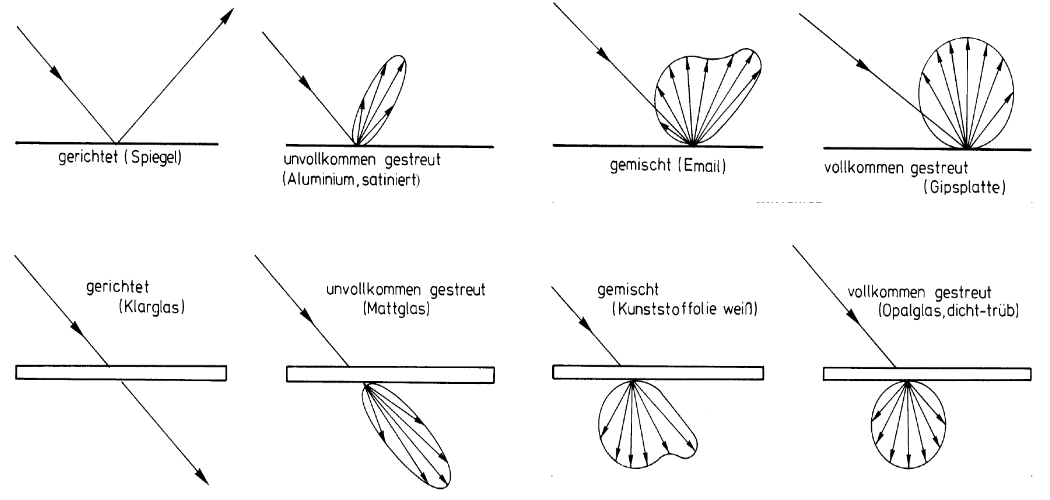
\includegraphics[width=0.9\textwidth]{bilder/reftrans} 
% Bilddatei aus dem Unterverzeichnis bilder holen, skalieren auf 0.8*Satzspiegel
\caption {Darstellung verschiedener Reflexion- (oben) und Transmissionsarten (unten) \protect\footnotemark}\label{b_reftrans}
\end{figure}

\footnotetext{\url{https://encrypted-tbn0.gstatic.com/images?q=tbn:ANd9GcQRXKyO2dzW7jXXbs_PqxZDRF2vKnJT-8qKf5w5mRAVG6SDatTk}}
 


\section{Lichtstrom $\Phi$} \label{sec_lumen}
Der Lichtstrom $\Phi$ steht für die Lichtleistung einer Lichtquelle und wird in der Einheit Lumen (lm) angegeben (Abbildung \ref{b_lumen}). $\Phi$ lehnt sich an der Helligkeitsempfindung des Auges an, der V($\lambda$)-Kurve (Kapitel \ref{sec_auge}). Daher sind Aussagen über die Strahlungsleistung in der Beleuchtungstechnik nur von peripherer Bedeutung\footnote{\cite[23]{ris}}. Man kann aber den Lichtstrom ins Verhältnis zur Strahlungsleistung setzten und so die Lichtausbeute $\eta$ in $\frac{lm}{W}$ berechnen\footnote{\cite[35]{greule}}. Mit dem $\eta$-Wert kann man aufzeigen wie effizient ein Leuchtmittel seine Strahlungsleistung in Lichtleistung umsetzt. Der Maximalwert von $\eta$ liegt bei $\eta_{max}=683$ $\frac{lm}{W}$ , dass nur durch eine monochromatisch grüne (555 nm) Lichtquelle erzeugt werden kann, weil dieses Licht am hellsten für das menschliche Auge ist\footnote{\cite[36]{greule}} (Kapitel \ref{sec_auge}).

\begin{figure}[H]     % h=here, t=top, b=bottom, p=page
\centering
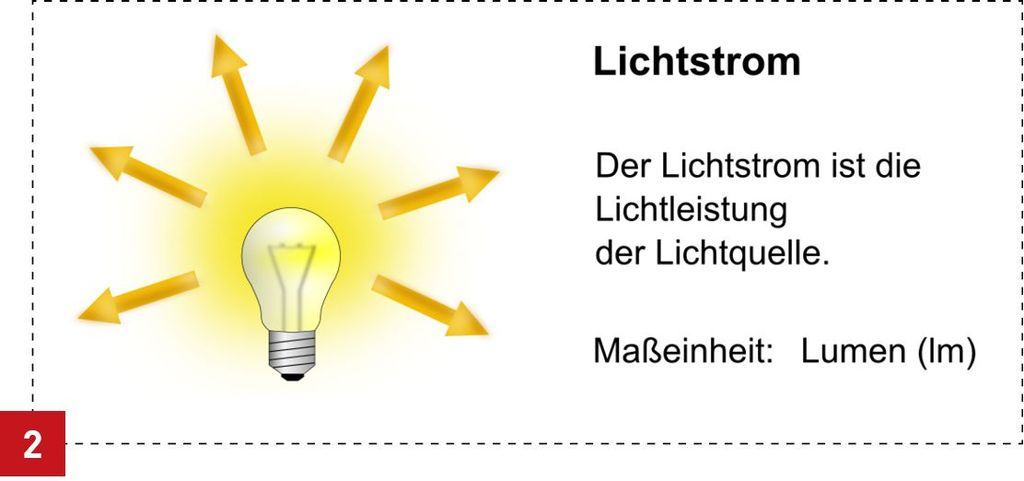
\includegraphics[width=0.7\textwidth]{bilder/lumen} 
% Bilddatei aus dem Unterverzeichnis bilder holen, skalieren auf 0.8*Satzspiegel
\caption {Der Lichtstrom gibt an, wie viel sichtbares Licht eine Lichtquelle abstrahlt. \protect\footnotemark}\label{b_lumen}
\end{figure}

\footnotetext{\url{https://www.sbz-online.de/Cache/GENTNER/10024/GV-SVG-EXPORT-20140303-1028_NTc4MTAwWg.JPG}}

Folgende Zahlen sind für Lichstromwerte typisch:
\newpage
\begin{table}[htp] 
		\rowcolors{1}{}{lgray} 
		\centering
		\begin{tabular}{rlcc}  % Spalten nach Ausrichtung: l, c, r, p{breite} 
		\toprule
		\multicolumn{3}{c}{\large\sffamily Lichtstrom}\\ 							
		\midrule
		Glühlampe & 230 V / 40 W & 415 lm\\ 
		Halogenglühlampe Niedervolt & 12 V / 50 W & 1.200 lm\\
		Halogenglühlampe Hochvolt & 230 V / 77 W & 1.320 lm\\
		Leuchtstofflampe & 230 V / 36 W & 3350 lm\\
		Natriumdampf-Niederdrucklampe & 230 V / 90 W & 13.500 lm\\
		Natriumdampf-Hochdrucklampe & 230 V / 100 W & 10.700 lm\\
		Halogenmetalldampflampe & 230 V / 100 W & 10.600 lm\\
		LED & 1 W & 50...> 150 lm\\
		\bottomrule
		\end{tabular}
		\caption{Verschiedene Beispiele für $\Phi$\protect\footnotemark}	
		\label{t_lumen}
	\end{table}
	\footnotetext{\cite[24]{ris}}


\section{Beleuchtungsstärke E}\label{sec_lux}
Die Beleuchtungsstärke E gibt an, wie groß ein Lichstrom $\Phi$ im Verhältnis zu seiner Lichtauftrittsfläche A ist  und wird in Lux (lx) angegeben\footnote{\cite[28]{ris}} (Gleichung \ref{gl_lux1}).
 \begin{equation}\label{gl_lux1}
	E=\frac{\Phi}{A}	
\end{equation}
Diese Formel gilt nur, solange die Fläche vom Lichtstrom senkrecht bestrahlt wird. Die Beleuchtungsstärke dient in der Innenraumbeleuchtung als ausschlaggebende Lichtkenngröße zur Einschätzung der Helligkeit. Dabei macht der E-Wert kaum eine Aussage über die mit dem Auge wahrgenommene Helligkeit\footnote{\cite[29]{ris}}. Eine doppelte so große Beleuchtungsstärke entspricht keines Wegs einer ebenso großen wahrgenommenen Helligkeitsänderung.

\begin{figure}[H]     % h=here, t=top, b=bottom, p=page
\centering
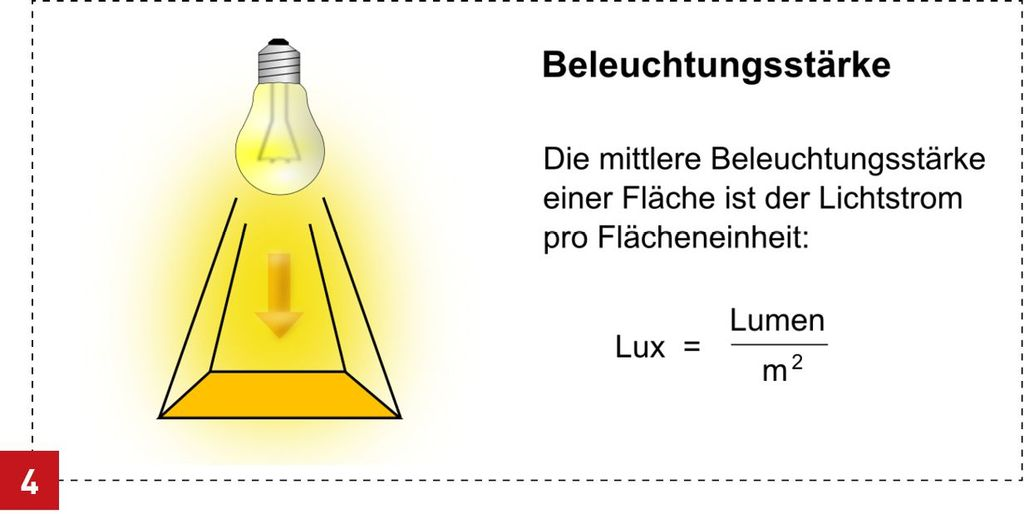
\includegraphics[width=0.7\textwidth]{bilder/lux} 
% Bilddatei aus dem Unterverzeichnis bilder holen, skalieren auf 0.8*Satzspiegel
\caption {Die Beleuchtungsstärke gibt an, wie viel Lichtstrom auf eine bestimme Fläche trifft.\protect\footnotemark}\label{b_lux}
\end{figure}

\footnotetext{\url{https://www.sbz-online.de/Cache/GENTNER/10024/GV-SVG-EXPORT-20140303-1028_NTc4MTAwWg.JPG}}

Folgende Zahlen sind typisch für die Beleuchtungsstärke:

\begin{table}[htp] 
		\rowcolors{1}{}{lgray} 
		\centering
		\begin{tabular}{rlcc}  % Spalten nach Ausrichtung: l, c, r, p{breite} 
		\toprule
		\multicolumn{2}{c}{\large\sffamily Beleuchtungsstärke}\\ 							
		\midrule
		wolkenloser Sommertag & 100.000 lx\\
		trüber Sommertag & 20.000 lx\\
		wolkenloser Wintertag & 400 lx\\
		Bürobeleuchtung & 500 lx\\
		Vollmondnacht & 0,3 lx\\
		Sternennacht & 0,01 lx\\
		\bottomrule
		\end{tabular}
		\caption{Verschiedene Beispiele für E\protect\footnotemark}	
		\label{t_lux}
	\end{table}
	\footnotetext{\cite[29]{ris}}
Die Beleuchtungsstärke spielt in der Lichtplanung eine sehr große Rolle. Mit ihr werden auch Gleichmäßigkeiten und Ungelichmäßigkeiten in der Beleuchtung bestimmt, die zum Beispiel für ausgeleuchtete Sportveranstaltung entscheidend sind.

\section{Lichtstärke I}\label{sec_candela}
Die Lichtstärke I zeigt auf, wie stark Licht in eine bestimme Richtung abgestrahlt wird und wird in Candela (cd) angegeben. I wird aus dm Verhältnis von Lichtstrom $\Phi$ zu dem bestrahlten Raumwinkel $/Omega$ errechnet\footnote{\cite[27]{ris}} (Gleichung \ref{gl_candela1}).
 \begin{equation}\label{gl_candela1}
	I=\frac{\Phi}{\Omega}	
\end{equation}
Der Raumwinkel $/Omega$ beschreibt die Beziehung zwischen eines Flächenausschnitts der Oberfläche einer dreidimensionalen Kugel zu dem Quadrat des Kugelradius und wird mit der Einheit Steradiant (sr) verwendet\footnote{\cite[26]{ris}}  (Gleichung \ref{gl_candela2}).
 \begin{equation}\label{gl_candela2}
	\Omega=\frac{A}{r^{2}}	
\end{equation}
Auf diese Weise kann die Verteilung des Lichtstroms $\Phi$ im Raum berechnet werden (Abbildung \ref{b_candela}).

 \begin{figure}[H]     % h=here, t=top, b=bottom, p=page
\centering
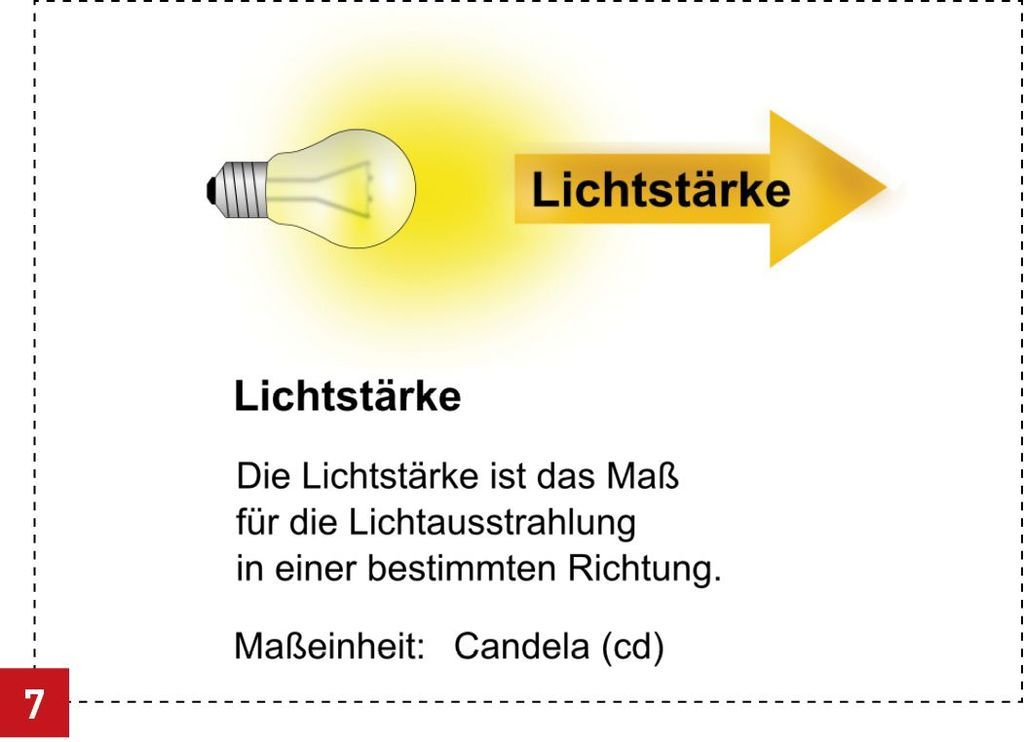
\includegraphics[width=0.7\textwidth]{bilder/candela} 
% Bilddatei aus dem Unterverzeichnis bilder holen, skalieren auf 0.8*Satzspiegel
\caption {Die Lichtstärke gibt an, wie viel Lichtstrom auf eine bestimme Richtung im Raum verteilt ist.\protect\footnotemark}\label{b_candela}
\end{figure}
\footnotetext{\url{https://www.sbz-online.de/Cache/GENTNER/10024/GV-SVG-EXPORT-20140303-1034_NTc4MTA2Wg.JPG}}

Typische Größen der Lichstärke sind:

\begin{table}[htp] 
		\rowcolors{1}{}{lgray} 
		\centering
		\begin{tabular}{rlcc}  % Spalten nach Ausrichtung: l, c, r, p{breite} 
		\toprule
		\multicolumn{2}{c}{\large\sffamily Lichtstärke}\\ 							
		\midrule
		Halogenglühlampe, 50W, HRI & 1.250.000 cd\\
		Leonardo De Sisti 1kW Halogenglühlampe &  115.250 cd\\
		Sonnenlicht & $2 \cdot 10^{27}$ cd\\
		\bottomrule
		\end{tabular}
		\caption{Verschiedene Beispiele für I\protect\footnotemark}	
		\label{t_candela}
	\end{table}
\footnotetext{\cite[36]{greule}}
Die Lichtstärke einer Kerze beträgt etwa 1 cd, wenn man davon ausgeht, dass sie in alle Richtungen gleichmäßig Licht ausstrahlt.\\
Mit sogenannten Lichtstärkeverteilungskurven (LVK) ist es möglich die Abstrahlcharakteristik einer Leuchte zu bestimmen und mit diesen Daten beispielweise 3D-Renderings einer Beleuchtungssituation zu simulieren. Dies ist jedoch für diese Arbeit nicht weiter interessant.

\section{Leuchtdichte L}\label{sec_candelamm}
Die Leuchtdichte L bewertet, wie hell eine beleuchtete oder selbstleuchtende Fläche von dem menschlichen Auge wahrgenommen wird und wird in $\frac{candela}{m^{2}}$ ($\frac{cd}{m^{2}}$) angegeben\footnote{\cite[34]{ris}}(Gleichung \ref{gl_candelamm1}).
 \begin{equation}\label{gl_candelamm1}
	L=\frac{I}{A}	
\end{equation}
Damit besteht mit der Leuchtdichte im Gegensatz zu den anderen Kenngrößen eine Verbindung zur tatsächlichen Wahrnehmung der Helligkeit. Zusätzlich ist die Leuchtdichte unabhängig von der Entfernung immer gleich hell(Abbildung \ref{b_candelamm}).

 \begin{figure}[H]     % h=here, t=top, b=bottom, p=page
\centering
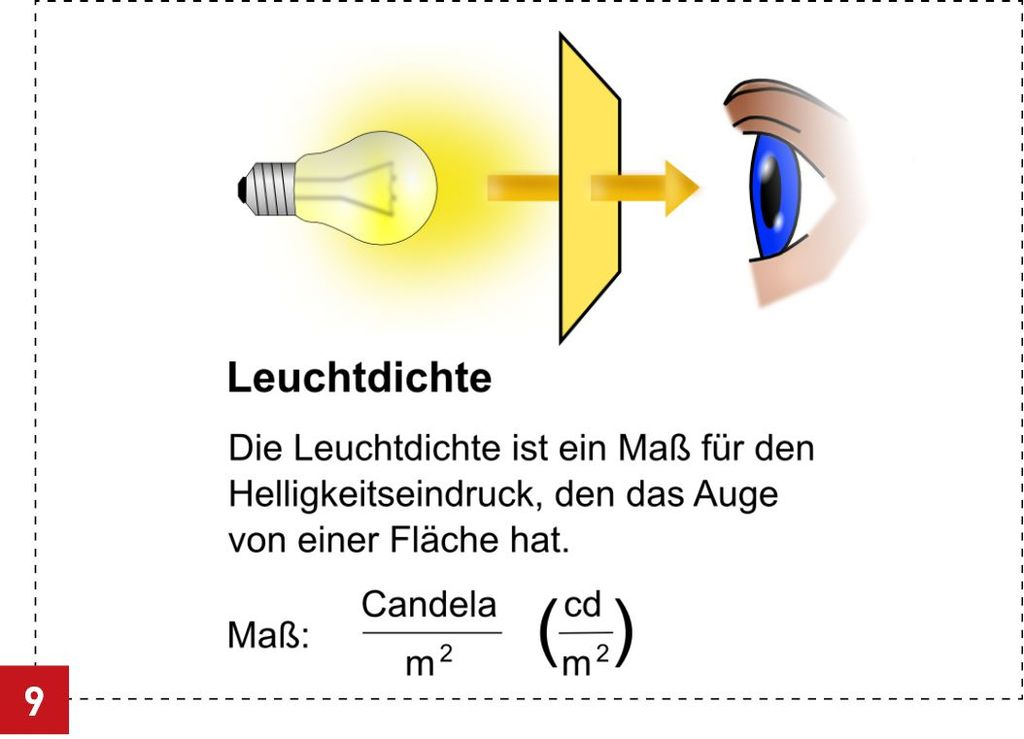
\includegraphics[width=0.7\textwidth]{bilder/candelamm} 
% Bilddatei aus dem Unterverzeichnis bilder holen, skalieren auf 0.8*Satzspiegel
\caption {Die Leuchtdichte hat einen Bezug auf die menschliche Helligkeitswahrnehmung.\protect\footnotemark}\label{b_candelamm}
\end{figure}
\footnotetext{\url{https://www.sbz-online.de/Cache/GENTNER/10024/GV-SVG-EXPORT-20140303-1034_NTc4MTA2Wg.JPG}}

Folgende Werte sind für die Leutdichte typisch:

\begin{table}[htp] 
		\rowcolors{1}{}{lgray} 
		\centering
		\begin{tabular}{rlcc}  % Spalten nach Ausrichtung: l, c, r, p{breite} 
		\toprule
		\multicolumn{2}{c}{\large\sffamily Leuchtdiche}\\ 							
		\midrule
		Fensteröffnung mittags, leichte Bewölkung & 5.000...50.000$\frac{candela}{m^{2}}$\\
		Fensteröffnung mittags, bedeckter Himmel & 1.000...3.000$\frac{candela}{m^{2}}$\\
		Sonnenscheibe mittags & 1,6...$10^{9}$ $\frac{candela}{m^{2}}$\\
		Vollmondscheibe & 2.500 $\frac{candela}{m^{2}}$\\
		Halogenglühlampe nackt & 20...$30 \cdot 10^{6}$ $\frac{candela}{m^{2}}$\\
		Leuchtstofflampe & 5.000...15.000 $\frac{candela}{m^{2}}$\\
		Weißes Papier bei 500 lx & 130...150 $\frac{candela}{m^{2}}$\\
		Umweltschutzpapier bei 500 lx & 90...150 $\frac{candela}{m^{2}}$\\
		\bottomrule
		\end{tabular}
		\caption{Verschiedene Beispiele für L\protect\footnotemark}	
		\label{t_candelamm}
	\end{table}
\footnotetext{\cite[35]{ris}}


\chapter{Leuchtmittel}
In diesem Kapitel werden verschiedene Leuchtmittel vorgestellt. Ein Augenmerk soll hier auf die LED-Leuchtmittel gelegt werden, da diese einen Hauptbestandteil der Thesisüberlegung betrifft.

%Aufteilung der Scheinwerfer in verschiedene Gruppen

\section{Glühlampe} \label{sec_glühlampe}
Die Glühlampe ist ein Temperaturstrahler. Sie besteht aus einem gasgefülltem Kolben, in dem ein Wolframwendel durch Stromzufuhr erhitzt wird. Der erhitzte Glühwendel erzeugt eine Farbtemperatur von ca. 3200K\footnote{\cite[137]{mueller}}. Der Großanteil des Lichtspektrums einer Glühlampe liegt im Infrarot-Bereich und wird damit in Wärme umgesetzt. Es werden also nur ca. 5\% bis 15\% der Leistung in Licht umgewandelt\footnote{\cite[78]{ris}}.
%Abbildung einfügen
Weil die Lichtausbeute $\eta$ von 10 $\frac{lumen}{Watt}$ bis 15 $\frac{lumen}{Watt}$ zu gering ist, wird die Glühlampe in der EU nicht mehr hergestellt\footnote{\cite[78]{ris}}.
 
\section{Halogenglühlampe} \label{sec_halogenglühlampe}
Auch die Halogenglühlampe ist ein Temperaturstrahler. Sie besteht auch Glaskolben und Woflramwendel, ist allerdings mit Jod oder einer Bromverbindung gefüllt\footnote{\cite[82]{ris}}.
Wenn nun der Wolframwendel erhitzt wird spalten sich Wolframatome vom Wendel ab. Diese Atome werden vom Jod respektive Brom gebunden und es entsteht ein Wolframhalogenid in dem Glaskolben. Wenn dieses Wolframhalogenid wiederum auf den erhitzen Wendel trifft, spaltet es sich in die Einzelteile auf. Das Wolfram gelangt zurück in den Wendel und der gasförmige Anteil fügt sich wieder in den Bereich des Glaskolben ein. Auf diese Weise entsteht ein Kreislauf, der der Halogenglühlampe effizienter als eine Glühlampe macht\footnote{\cite[83-84]{ris}} (Abbildung \ref{b_halogenkreis}).

\begin{figure}[htp]     % h=here, t=top, b=bottom, p=page
\centering
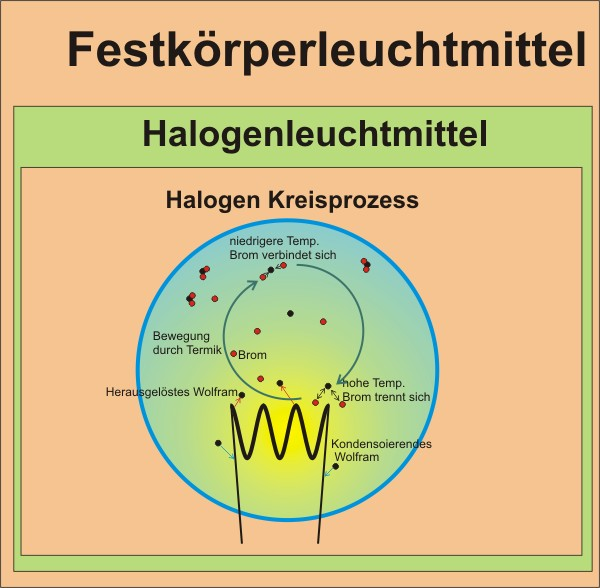
\includegraphics[width=0.7\textwidth]{bilder/halogenkreis} 
% Bilddatei aus dem Unterverzeichnis bilder holen, skalieren auf 0.8*Satzspiegel
\caption {Darstellung des Halogen Kreisprozesses\protect\footnotemark}\label{b_halogenkreis}
\end{figure}
\footnotetext{\url{https://www.haustechnikdialog.de/SHKwissen/Images/Leuchtmittelhalogenkreisprozess-Bernstaedt.jpg}}

\noindent Die Lichtausbeute einer 50 W Halogenglühlampe beträgt beispielsweise $\eta=18$ $\frac{lumen}{Watt}$ \footnote{\cite[35]{greule}}.

\section{Entladungslampen} \label{sec_entladungslampe}
Entladungslampen erzeugen Licht durch eine angelegte Spannung an einem ionisierten Gasgemisch in einem Glaskolben. Abhängig von dem Gasgemisch entsteht dabei eine Lichtfarbe.\footnote{\cite[140]{mueller}}. Man kann die Entladungslampen grob in zwei Kategorien einteilen: die Niederdruck-Entladungslampen und die Hochdruck-Entladungslampen.\\

\noindent Niederdruckentladungslampen haben einen Druck von ca. $10^{-6}$ bar. Ihr Gasgemisch besteht aus neutralen Atomen, geladenen Ionen und freien Elektronen. Dieses Gasgemisch befindet sich in einem Glasrohr. An den beiden Enden des Glasrohres liegen Elektroden an. Wenn diese mit einer Spannung versorgt werden, ziehen sich die negativen Elektronen zu der positiven Elektrode. Die positiven Ionen verhalten sich umgekehrt und wandern zur negativen Elektrode. Dabei treffen die herumschwirrenden Elektronen und Ionen auf neutrale Gasatome. Die Elektronen der Gasatome werden von ihrer Bahn abgedrängt und dabei wird Energie in Form von Strahlung frei\footnote{\cite[93]{ris}} (Abbildung \ref{b_leuchtstoff}). Damit es während des Betriebs nicht zum Kurzschluss kommt, wird der Strom durch beispielsweise induktive Vorwiderstände gedrosselt.\footnote{\cite[141]{mueller}}\\
Bei der Leuchtstoffröhre beispielsweise erzeugt das Quecksilbergasgemisch UV-Strahlung (253,7 nm), die nicht vom menschlichen Auge erkennbar ist. Erst wenn diese UV-Strahlung auf die Leuchtschicht am Röhrenrand trifft strahlt diese ein sichtbares Licht ab. Dabei wird nur ein Teil dieser UV-Strahlung in sichtbares Licht umgesetzt (Abbildung \ref{b_leuchtstoff}).\footnote{\cite[96]{ris}}

\begin{figure}[htp]     % h=here, t=top, b=bottom, p=page
\centering
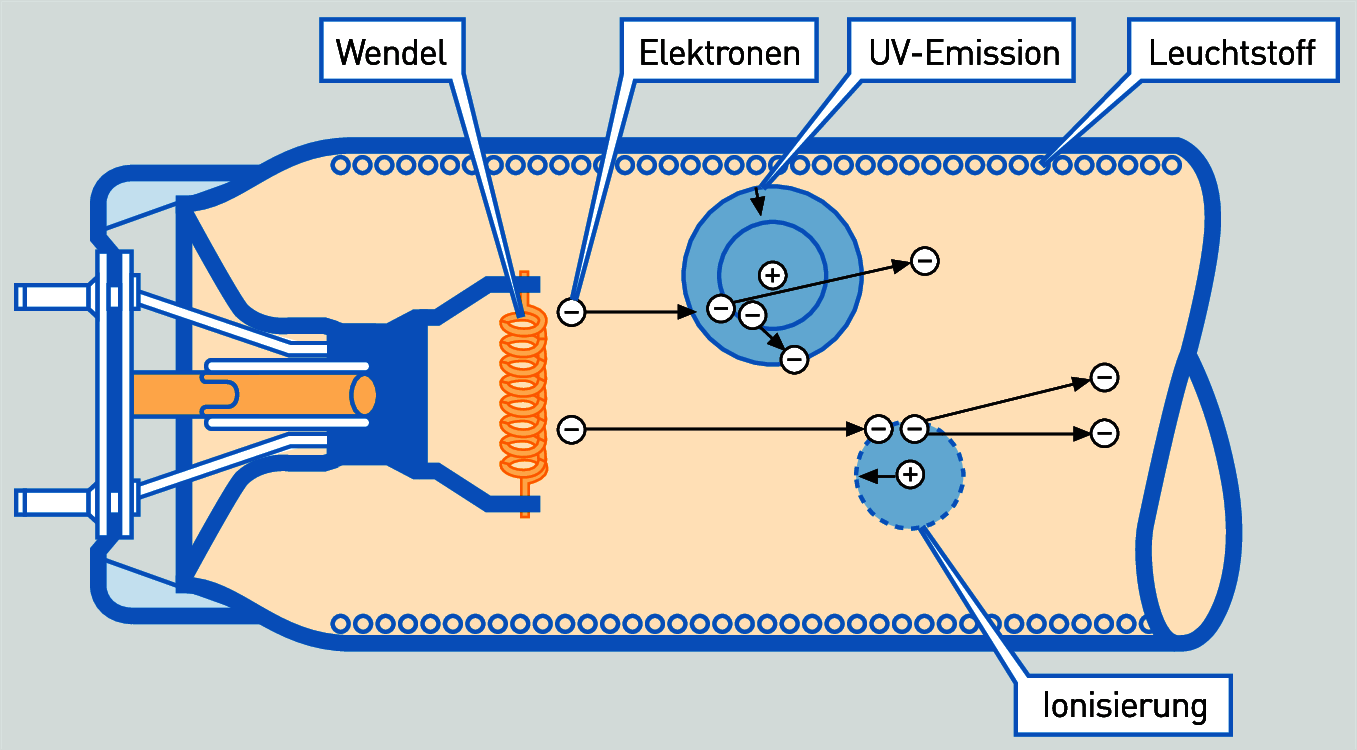
\includegraphics[width=0.7\textwidth]{bilder/leuchtstoff} 
% Bilddatei aus dem Unterverzeichnis bilder holen, skalieren auf 0.8*Satzspiegel
\caption {Aufbau einer Leuchtstoffröhre\protect\footnotemark}\label{b_leuchtstoff}
\end{figure}
\footnotetext{\url{https://www.trilux.com/de/beleuchtungspraxis/fileadmin/user_upload/Abb_LL_Funktion.pdf.png}}

\noindent Leuchtstofflampen erreichen eine Lichtausbeute $\eta$ von bis zu 116 $\frac{lumen}{Watt}$.\\

\noindent Hochdruckentladungslampen dagegen nutzen einen Druck von 0,3 bar bis 10 bar. Sie sind von der Funktionsweise her ähnlich wie die Niederdruckentladungslampen, bestehen aber aus einem kleinem Glaskolben, da eine lange Glasröhre dem Druck nicht standhält (Abbildung \ref{b_hochdruck}). Wenn bei einer Halogen-Metalldampflampe beispielsweie eine Spannung an den Elektroden anliegt entsteht zwischen den beiden Elektroden ein Lichtbogen. Dieser Lichtbogen regt dann das Gasgemisch der Lampe an und gibt dem Licht so eine Lichtfarbe\footnote{\cite[129]{ris}}.
Hochdruckentladungslampen brauchen für den Zündvorgang ein Vorschaltgerät, um die hohe Initialspannung generieren zu können. Nach der Zündung braucht die Lampe ca. 3 min bis 5 min bis sie ihren vollen Wirkungsgrad erreicht hat. Das Gasgemisch muss nach dem Ausschalten der Lampe erst wieder abkühlen und so dauert es bis zu 20 Minuten, bis die Lampe erneut genzündet werden kann\footnote{\cite[147]{mueller}}.

\begin{figure}[htp]     % h=here, t=top, b=bottom, p=page
\centering
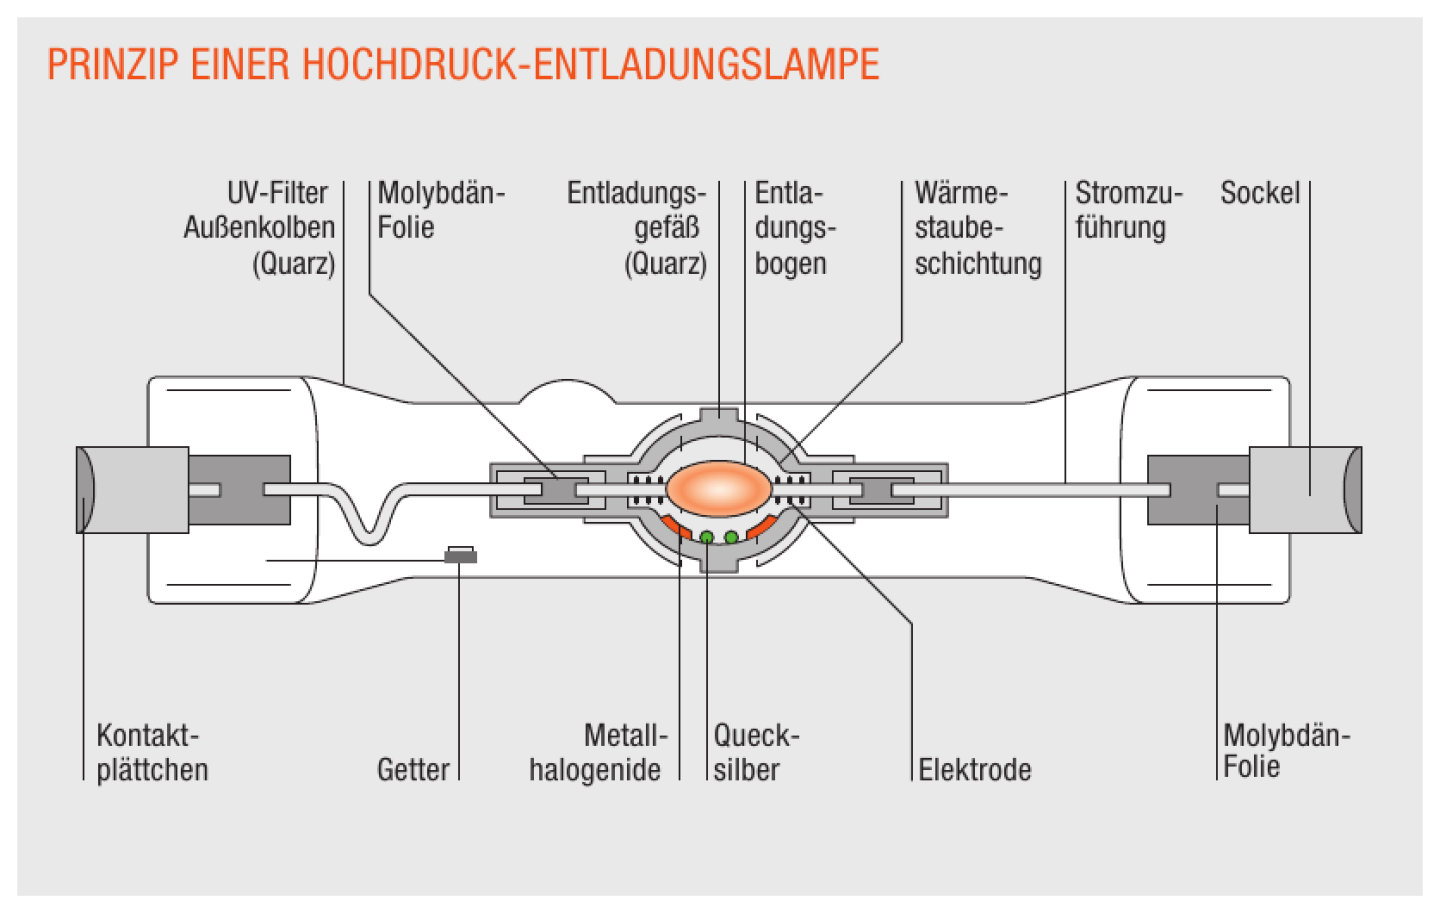
\includegraphics[width=0.9\textwidth]{bilder/hochdruck} 
% Bilddatei aus dem Unterverzeichnis bilder holen, skalieren auf 0.8*Satzspiegel
\caption {Aufbau einer Hochdruckentladungslampe\protect\footnotemark}\label{b_hochdruck}
\end{figure}
\footnotetext{\url{https://dammedia.ledvance.info/media/img/asset-296401/s,x,1440,y,0/334675.jpg}}
\noindent Eine Halogenmetalldampflampe hat eine Lichtausbeute $\eta$ von beispielsweise 70 $\frac{lumen}{Watt}$.

\section{LEDs} \label{sec_led}
Light-Emitting Diode sind heutzutage die modernsten Leuchtmittel. Mit LEDs werden immer mehr konventionelle Leuchtmittel ersetzt, weil sie große Vorteile, wie ein niedrigen Stormverbrauch und ein sehr hohe Lichtausbeute mit sich bringen. LEDs nutzen elektrische Spannung, um ihr  Halbleitermaterial zum Leuchten zu bringen. \footnote{\cite[150]{mueller}}. Da sich die Halbleiterbauelemente wie eine Diode verhalten ist ein Strom, der in Durchlassrichtung fließt, nötig, damit die LED Licht abstrahlt. Rote und Gelbe LED werden aus Aluminium-Indium-Galliumphosphid (AllnGaP) hergestellt und grüne und blaue LED aus Indium-Gallium-Nitrid (InGaN)\footnote{\cite[153]{ris}}.\\
Das lichterzeugende Element der LED ist meistens in der Vertiefung eines Metallhalters angebracht. Das austretende Licht wird auch an den Rändern dieser Vertiefung reflektiert. Die Lötstelle des Metallhalters wird als elektrischer Anschluss der LED genutzt, während der Metallhalter selbst als Katode fungiert. Mit einem Draht aus Gold wird die Oberseite des lichterzeugenden Elements verbunden und als Anode für den Stromfluss genutzt\footnote{\cite[154]{ris}} (Abbildung \ref{b_led}). Die LED wird schließlich von einer Sekundäroptik ummantelt. Diese Optik sorgt dafür, dass das LED Licht nicht mehr zur Seite austritt und gebündelt wird.

\begin{figure}[htp]     % h=here, t=top, b=bottom, p=page
\centering
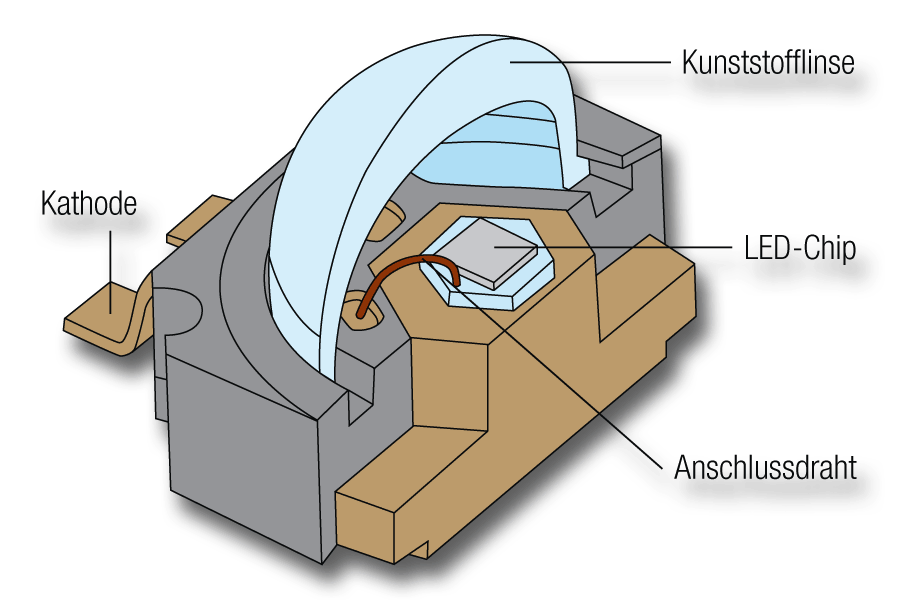
\includegraphics[width=0.7\textwidth]{bilder/led} 
% Bilddatei aus dem Unterverzeichnis bilder holen, skalieren auf 0.8*Satzspiegel
\caption {Aufbau einer LED\protect\footnotemark}\label{b_led}
\end{figure}
\footnotetext{\url{https://www.energy-innovation-austria.at/wp-content/uploads/2014/12/4_14_s3_lichtwissen17_LED_grafik2.png}}


\noindent Je nachdem welche der genannten Stoffe in der LED verwendet werden, leuchtet die LED in einer bestimmten Farbe monochromatisch. Um weißes Licht zu erzeugen, gibt es zwei Varianten\footnote{\cite[151-152]{mueller}}:

\begin{itemize}
\item MultiLED: Bei dieser Methode werden drei LEDs mit der Farbe rot, grün und blau in einem Gehäuse verbaut. Zusammen ergeben sie ein weißes Licht. Da das Spektrum des Lichts aber nicht nur aus diesen drei Farben besteht, werden beispielsweise Pastelltöne unter diesem weiß nicht natürlich aussehen. Man verliert also deutlich an Qualität der Farbwiedergabe

\item Phosphor Methode: Bei dieser Methode wird eine blaue LED von einer gelben Phosphorschicht ummantelt. Wenn die LED leuchtet wird entweder das blaue Licht durchgelassen oder die Phosphorschicht angeregt und gelbes Licht erzeugt. Diese beiden Lichtfarben mischen sich und weißes Licht wird erzeugt (Abbildung \ref{b_ledw}). Dieses Licht hat eine deutlich höhere Qualität der Farbwiedergabe, hat aber eine Schwäche im roten Spektralbereich. Die Herstellung phosphorbeschichter blauer LEDs hat sich in der Branche durchgesetzt.
\end{itemize}

\begin{figure}[htp]     % h=here, t=top, b=bottom, p=page
\centering
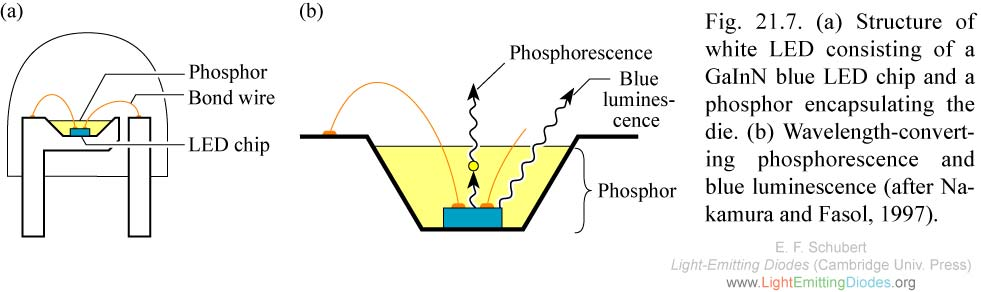
\includegraphics[width=1.0\textwidth]{bilder/ledw} 
% Bilddatei aus dem Unterverzeichnis bilder holen, skalieren auf 0.8*Satzspiegel
\caption {Aufbau einer weißen LED\protect\footnotemark}\label{b_ledw}
\end{figure}
\footnotetext{\url{https://www.ecse.rpi.edu/~schubert/Light-Emitting-Diodes-dot-org/chap21/F21-07\%20Nichia\%20wh\%20LED\%20structu.jpg}}

\noindent LEDs verlieren mit der Zeit durch die Hitze an Qualität. Scheinwerferhersteller versuchen durch komplexe Algorithmen für die LEDs diesen Qualitätsverlust zu kompensieren. Ebenso gibt es herstellungsbedingte Abweichungen bei LED's. Da die Vorgänge sehr kompliziert sind, werden die LED's nach der Herstellung in sogenannte Binnings eingeteilt. In einem Binnig sind also jeweils die LED's mit den ähnlichsten Eigenschaften zusammengefasst, so dass beim Scheinwerferbau nur sich sehr ähnliche LED's verwendet werden\footnote{\cite[153]{mueller}}.

%Für Scheinwerfer im Veranstaltungsbereich werden mittlerweile verschiedene LED-Leuchtmittel verwendet. Am Anfang waren Scheinwerfer typisch, die mit einem RGB-Modul bestückt waren. Farben sind mit diesen Scheinwerfern gut darstellbar, ein gemischtes RGB-Weißlicht hingegen hat keine akzeptable Qualitität. Scheinwerfer mit RGBW LEDs stellen eine Verbesserung der Weißlichtqualität dar, können aber damit immernoch das sichtbare Spektrum füllen. Daher gehen Scheinwerferhersteller dazu über Scheinwerfer mit noch mehr farbenen LEDs zu bauen (Multichip). So hat der Clay Paky K-Eye K20 beispielsweise 6 LEDs mit Rot, Grün, Blau, Lime, Amber und Cyan. Das daraus resultierende Spektrum hat eine hohe Farb- und Unbuntqualität. Andere Scheinwerfer setzten wiederum auf eine reinweiße LED-Engine mit nur weißen LEDs. Der Martin Mac Encore Wash CLD beispielsweise erreicht mit seiner LED-Engine die noch zusätzlich ein CMY-Mischung hat auch hohe Farb- und Unbuntquälitäten.  
%drüber gucken



\section{Farbtemperatur} \label{sec_farbtemperatur}
Mit der Farbtemperatur lässt sich die Qualität des Lichts 
bestimmen. Entstanden ist der Begriff durch die Untersuchen von Lord Kelvin. Er hat herausgefunden, dass es eine Verbidnung zwischen der Temperatur eines schwarzes Strahlers (Plank'scher Strahler) und dessen Lichtfarbe gibt\footnote{\cite[89]{mueller}}. Daher wird die Farbtemperatur einer Lampe stets in Kelvin (K) angegeben. Bei den Untersuchen wird ein schwarzer Körper mit einem Hohlraum erhitzt. Dadurch wird aus diesem Hohlraum Licht abgestrahlt. Ändert sich die Temperatur des schwarzen Körpers, so ändert sich auch das Spektrum des abgestrahlten Lichts (Abbildung \ref{b_cct2}).

\begin{figure}[H]     % h=here, t=top, b=bottom, p=page
\centering
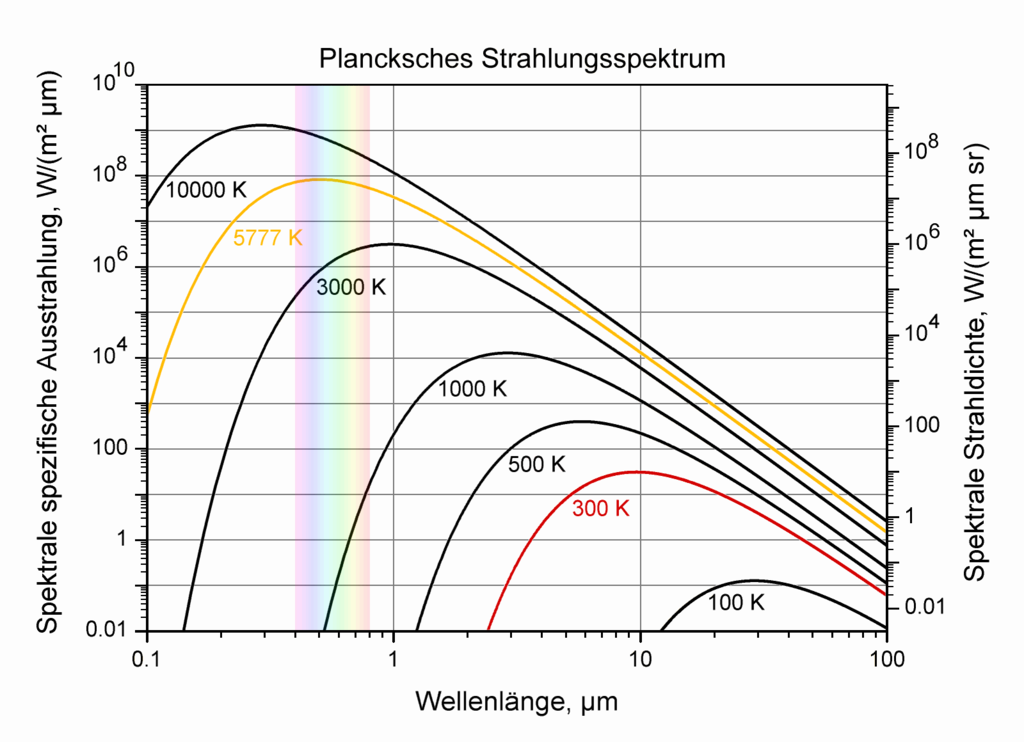
\includegraphics[width=0.9\textwidth]{bilder/cct2} 
% Bilddatei aus dem Unterverzeichnis bilder holen, skalieren auf 0.8*Satzspiegel
\caption {Spektrale Kurven verschiedener Farbtemperaturen des schwarzen Strahlers. (Der bunteingefärbte Bereich stellt das sichtbare Lichtspektrum dar.)\protect\footnotemark}\label{b_cct2}
\end{figure}
\footnotetext{\url{https://upload.wikimedia.org/wikipedia/commons/thumb/0/0e/BlackbodySpectrum_loglog_150dpi_de.png/640px-BlackbodySpectrum_loglog_150dpi_de.png}}

Die abgestrahlte Lichtfarbe des schwarzen Strahlers ist anfänglich rötlich wechselt bei steigenden Temperatur des Körpers ins weiße und wird danach immer bläulicher. Daher spricht man bei einer hohen Farbtemperatur von einer kalten Lichtfarbe und bei niedriger Farbtemperatur von einer warmen(Abbildung \ref{b_cct1}). Wenn das Licht einer Lampe von der spektralen Beschaffenheit mit dem Licht des schwarzen Strahlers übereinstimmt, wird die Lichtfarbe der Temperatur des Schwarzen Körpers zugeordnet\footnote{\cite[89]{mueller}}.

\begin{figure}[H]     % h=here, t=top, b=bottom, p=page
\centering
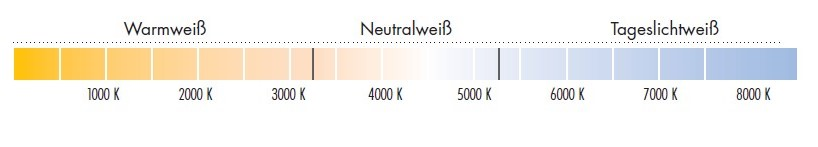
\includegraphics[width=1.0\textwidth]{bilder/cct1} 
% Bilddatei aus dem Unterverzeichnis bilder holen, skalieren auf 0.8*Satzspiegel
\caption {Spektrale Kurven verschiedener Farbtemperaturen des schwarzen Strahlers. (Der bunteingefärbte Bereich stellt das sichtbare Lichtspektrum dar.)\protect\footnotemark}\label{b_cct1}
\end{figure}
\footnotetext{\url{http://www.ledmarkt24.de/bilder/content/led-farbtemperatur-warmweiss-neutral.jpg}}



Typische Farbtemperaturen sind:

\begin{table}[htp] 
		\rowcolors{1}{}{lgray} 
		\centering
		\begin{tabular}{rlcc}  % Spalten nach Ausrichtung: l, c, r, p{breite} 
		\toprule
		\multicolumn{2}{c}{\large\sffamily Farbtemperatur}\\ 							
		\midrule
		Kerzenlicht & 1850 K\\
		Glühlampe 40W & 2650 K\\
		Normlicht A & 2855,4 K\\
		Halogenglühlampe & 3200 K\\
		Normlicht D65, Fernsehweißbild (Europa) & 6504 K\\
		Tageslicht bei bedecktem Himmel & 6700 K - 7000 K\\
		blauer Himmel ohne direkte Sonne & 12.000 K - 30.000 K\\
		\bottomrule
		\end{tabular}
		\caption{Verschiedene Beispiele für die Farbtemperatur\protect\footnotemark}	
		\label{t_candela}
	\end{table}
\footnotetext{\cite[29]{greule}}


Falls das Spektrum einer Lampe sehr von dem des Schwarzen Strahlers abweicht, kann eigentlich keine vernünftige Aussage über die Farbtemperatur der Lampe gemacht werden. Damit man trotzdem Gasentladungslampen und LED's eine Farbtemperatur zuordnen kann, wird dem Spektrum eine korrelierte Farbtemperatur zugeordnet. Diese \glqq Correlated Color Temperatur\grqq\ (CCT) macht eine Aussage darüber, welche Farbtemperatur der Leuchte am ähnlichsten ist\footnote{\cite[91]{mueller}} (Kapitel \ref{sec_xyz}).

\chapter{Farben}

%Einleitung vernünftig schreiben

\section{Farben mit dem Auge sehen} \label{sec_auge}
% Einleitender Satz fehlt

Es gibt zwei verschiedene Fälle, in denen der Mensch die Gesichtsemfpindung Farbe verspürt: Zum einen leuchtet ein Objekt von selbst, sodass dessen Licht ins Auge gelangt. Aus dem sichtbaren Spektralbereich des Lichtspektrums erzeugt dann die Netzhaut im Zusammenspiel mit dem Gehirn ein Farbreiz $\phi(\lambda)$. In diesem Fall nennt man das Objekt einen Selbstleuchter. Zum anderen wird das Objekt von einer Lichtquelle beleuchtet und das reflektierte Lichtspektrum wahrgenommen. Der Gegenstand aborbiert und transmittiert bestimme spektrale Anteile des Lichts und reflektiert den für den Farbton verantworlichen Rest (Kapitel \ref{chap_grundlagen}). Daher erscheint beispielsweise ein roter Apfel von blauem Licht beleuchtet unbunt, da kein roter Spektralanteil im blauen Licht vorhanden ist.
In diesem zweiten Fall spricht man von Körperfarben\footnote{\cite[103]{hentschel}}.\\     
Damit ein Mensch so einen Farbreiz wahrnehmen kann, gibt es im Auge zwei Arten von lichtempfindlichen Rezeptoren in der Netzhaut, die für unsere Farbwahrnehmung verantwortlich sind: Zapfen und Stäbchen.\\
Die Stäbchen nehmen verschiedene Helligkeitseindrücke wahr, können aber keine Farben unterscheiden. Daher sind sie für das skotopische Sehen (Nachtsehen) von $3 \cdot 10^{-6}$ $\frac{cd}{m^{2}}$ bis 0,03 $\frac{cd}{m^{2}}$ verantwortlich\footnote{\cite{doccheck sko}}.
Die verschiedenen spektralen Anteile des Lichts wirken sich auf die Zapfen aus und verantworten so den Farbeindruck. Sie sind für das photopische Sehen (Tagessehen) ab einer Leuchtdichte von 3 $\frac{cd}{m^{2}}$ zuständig \footnote{\cite{doccheck pho}}.\\
Das menschliche Auge kann Wellenlängen von 380 nm bis 780 nm wahrnehmen. Jedoch ist das Auge nicht für alle Farben gleich empfindlich. Grüne Gegenstände (bspw. 555 nm) wirken immer heller als blaue (bspw. 485 nm) oder rote (bspw. 680 nm). Dieser Sachverhalt wurde mit der V($\lambda$)-Kurve aufgezeigt (Abbildung \ref{b_augespek}).

\begin{figure}[htp]     % h=here, t=top, b=bottom, p=page
\centering
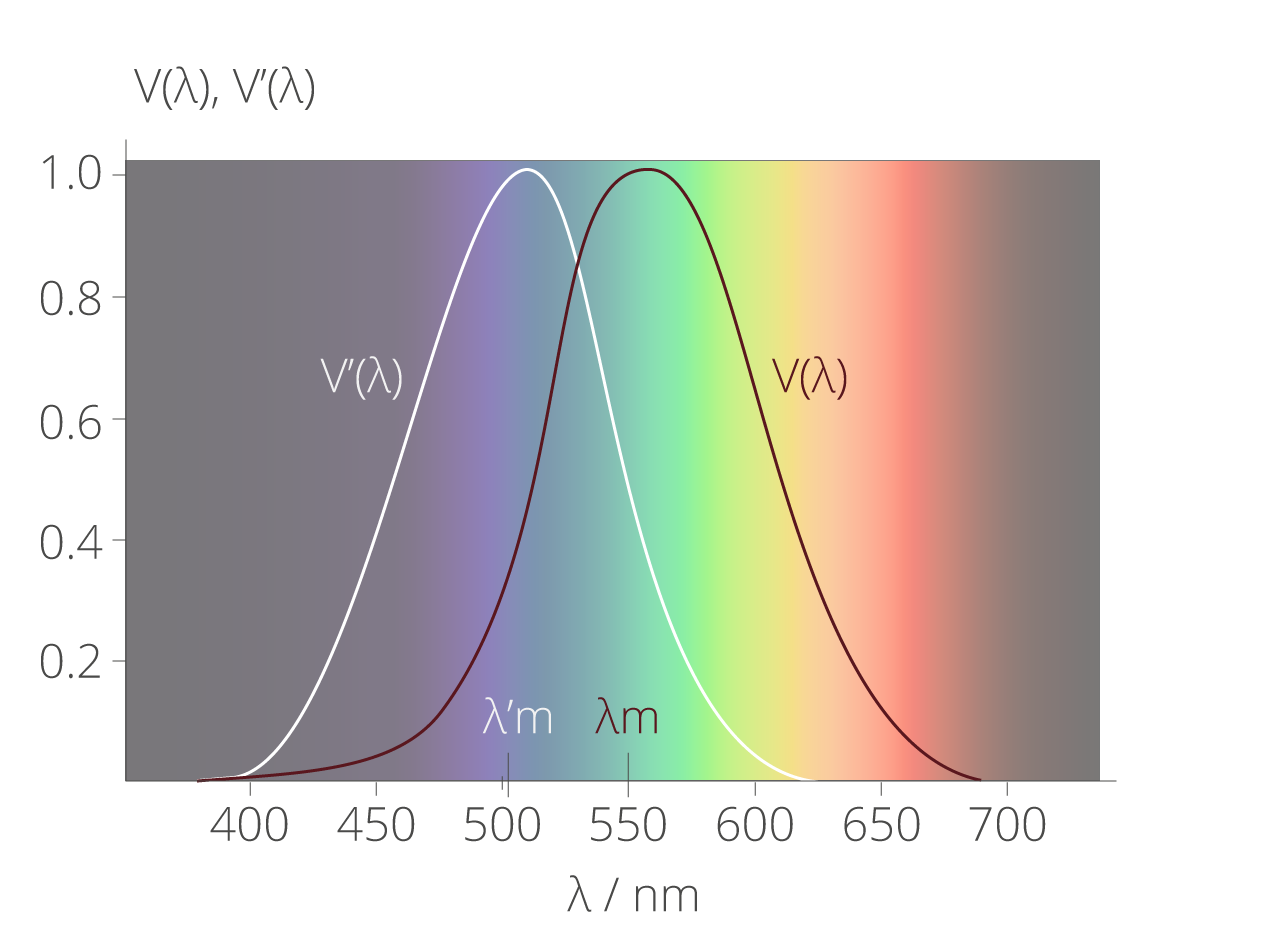
\includegraphics[width=0.7\textwidth]{bilder/augespek} 
% Bilddatei aus dem Unterverzeichnis bilder holen, skalieren auf 0.8*Satzspiegel
\caption {Die V($\lambda$)-Kurve zeigt, wie das Auge die verschiedenen Wellenlänge beim photopischen Sehen gewichtet. Die weiße Kurve (V'($\lambda$)) beschreibt, wie sich das Farbsehen beim Nachtsehen verschiebt. \protect\footnotemark}\label{b_augespek}
\end{figure}

\footnotetext{\url{https://www.gigahertz-optik.de/assets/Uploads/Abb.-II.13-neu-v03.png}}

\noindent Mit den Zapfen und Stäbchen kann ein Mensch bis zu 200 verschiedene Farbtöne wahrnehmen. Wenn man die verschiedenen möglichen Helligkeiten und Weißkombinationen dieser Farbtöne zusätzlich in Betracht zieht, kann von ca. 20 Millionen unterschiedlichen Farben gesprochen werden, die ein Mensch wahrnehmen kann \footnote{\cite{unimann}}.



\section{Theorien der Farbwahrnehmung}
\label{sec_colour}
 
Um all diese Farben unterscheiden zu können gibt es nach Thomas Young und Hermann von Helmholtz drei Rezeptortypen. Die \glqq Trichromatische Theorie\grqq\ besagt, dass es grüne, blaue und rote Zapfen gibt, die unterschiedlich empfindlich für die jeweiligen Spektralanteile des Lichtes sind. Aus diesen drei Farbinformation (RGB-Werte) entsteht dann im Gehirn eine Farbe. Die RGB-Zapfen nehmen tatsächlich ganze Bereiche des Spektrums wahr und daher kann man diese eher als Short-, Middle- und Long-Zapfen betiteln\footnote{\cite[62-63]{greule}} (Abbildung \ref{b_sml}).

\begin{figure}[H]     % h=here, t=top, b=bottom, p=page
\centering
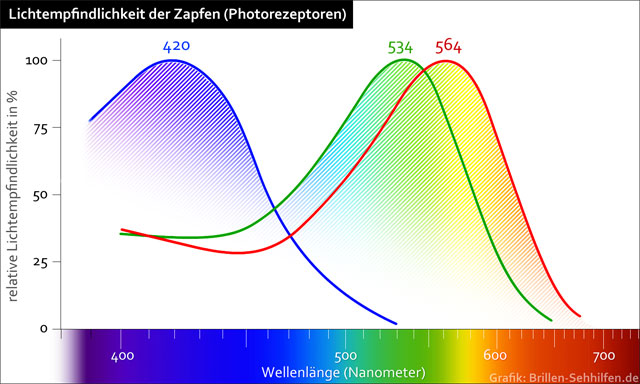
\includegraphics[width=0.7\textwidth]{bilder/sml} 
% Bilddatei aus dem Unterverzeichnis bilder holen, skalieren auf 0.8*Satzspiegel
\caption {Die Kurven zeigen die Empfindlichkeiten der S-Zapfen (blau), der M-Zapfen (grün) und der L-Zapfen (rot) und ihre Maxima. Auffällig ist, dass sich die Bereiche der M- und L-Zapfen größtenteils überlappen und die Zapfen für den (tief)roten Spektralbereich kaum empfindlich sind.\protect\footnotemark}\label{b_sml}
\end{figure}

\footnotetext{\url{https://www.brillen-sehhilfen.de/auge/images/farbensehen-wellenlaengen-zapfen-1.jpg}}

\noindent Auf diese Weise lassen sich aber nicht alle Phänomene der Farbwahrnehmung erklären. 1878 hat Ewald Hering eine andere Theorie entwickelt, wie Farben wahrgenommen werden und diese \glqq Gegenfarbentheorie\grqq\ genannt. Die Theorie besagt, dass es immer zwei Farben gibt, die sich gegensätzlich verhalten: rot und grün, blau und gelb und der unbunte Gegensatz schwarz (dunkel) und weiß (hell).\\ Nach ein paar Jahren der Uneinigkeit, welche der genannten Theorien korrekt ist, hat 1905 Johannes v. Kries mit seiner \glqq Zonentheorie\grqq\ herausgestellt, dass beide Theorien zugleich zutreffen. In der ersten Zone wird im Auge nach der \glqq Trichromatische Theorie\grqq\ eine Farbe als RGB-Stimulus wahrgenommen, dieser wird dann in der zweiten Zone nach der \glqq Gegenfarbentheorie\grqq\ im Gehirn mit den drei Farbgegensätzen ausgewertet\footnote{\cite[104]{hentschel}} (Abbildung \ref{b_zonen}).
 
\begin{figure}[H]     % h=here, t=top, b=bottom, p=page
\centering
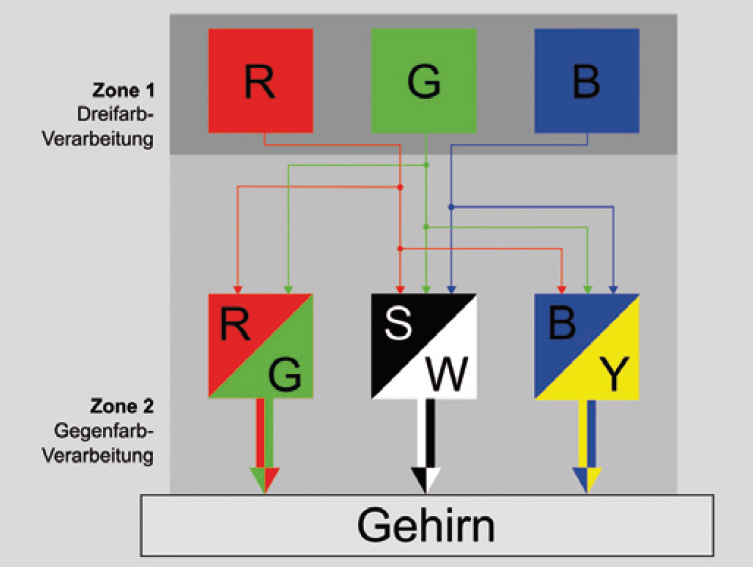
\includegraphics[width=0.7\textwidth]{bilder/zonen} 
% Bilddatei aus dem Unterverzeichnis bilder holen, skalieren auf 0.8*Satzspiegel
\caption {Darstellung der \glqq Zonentheorie\grqq\ von v. Kries \protect\footnotemark}\label{b_zonen}
\end{figure}
\footnotetext{\cite[153]{greule}}

\section{Farbmischung} \label{sec_farbmischung}
Bei der additiven Farbmischung werden die Spektralanteile verschiedener Farbtöne als Mischfarbe erkannt. Dies kann auf unterschiedliche Weisen passieren. Entweder treffen zwei verschiedene Spektralanteile auf den gleichen Punkt auf der Netzhaut und lösen so einen Farbreiz aus. Oder das Licht verschiedener Wellenlängen trifft auf unterschiedliche Teile der Netzhaut, die so dicht aneinander sind, dass das Auge daraus eine Farbe mischt (örtliche Nähe). Oder derselbe Punkt auf der Netzhaut wird von zwei verschiedenen Spektralanteilen mit einer Wechselfrequenz von $f\geq25Hz$ getroffen (zeitliche Nähe). Oder das Licht verschiedener Wellenlängen trifft auf unterschiedliche Teile der Netzhaut, die so dicht aneinander sind, dass das Auge daraus eine Farbe mischt.\\
Grundsätzlich werden bei jeder Art der additiven Farbmischung die Strahlungsleistungen der Spektralanteile $\Phi_{e\lambda,i}(\lambda)$ zusammenaddiert\footnote{\cite[83]{greule}} (Gleichung\ref{gl_farbe+}).

	\begin{equation}\label{gl_farbe+}
		\Phi_{e\lambda}(\lambda) = \Phi_{e\lambda,1}(\lambda) + \Phi_{e\lambda,2}(\lambda) + \Phi_{e\lambda,3}(\lambda)
	\end{equation}
\newpage
1853 hat Grassmann zur additiven Farbmischung vier allgemein gültige Regeln aufgestellt: 

\begin{itemize}
\item Die erste Regel besagt, daß \emph{\glqq jeder Farbeindruck der genannten Art sich in drei mathematisch bestimmbare Momente zerlegt: den Farbenton, die Intensität der Farbe und die Intensität des beigemischten Weiß.\grqq} \citep[70]{grassmann}
\item Die zweite Regel besagt, \emph{\glqq daß, wenn man von den beiden zu vermischenden Lichtern das eine stetig ändert (während das andere unverändert bleibt), auch der Eindruck der Mischung sich stetig ändert.\grqq} \citep[72]{grassmann}
\item Die dritte Regel besagt, \emph{\glqq daß zwei Farben, deren jede constanten Farbenton, constante Farbenintensität und constante Intensität des begemischten Weiß hat, auch constante Farbenmischung geben, gleich viel aus welchen homogenen Farben jene zusammengesetzt seyen.\grqq} \citep[78]{grassmann}
\item Die vierte Regel besagt, \emph{\glqq daß die gesammte Lichtintensität der Mischung die Summe sey aus den Intensitäten der gemischten Lichter.\grqq} \citep[82]{grassmann}

\end{itemize}

Die erste Regel besagt, dass die additive Farbmischung beispielsweise über Farbton, Sättigung und Helligkeit (Weißheit) definiert werden kann. Drei Angaben eines Farbeindrucks reichen also aus, eine Farbe eindeutig zu beschreiben\footnote{\cite[105]{hentschel}}. Dies kann auch über die RGB-Werte (Kapitel \ref{sec_rgb}) oder Primärvalenzen geschehen (Kapitel \ref{sec_xyz}). In der Abbildung \ref{b_farben+} ist dargestellt, wie aus den RGB-Grundfarben die additiven Mischfarben entstehen.

\begin{figure}[H]     % h=here, t=top, b=bottom, p=page
\centering
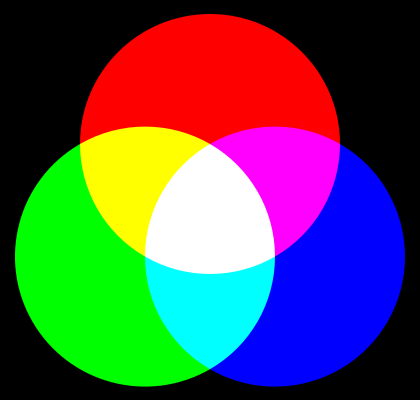
\includegraphics[width=0.5\textwidth]{bilder/farben+} 
% Bilddatei aus dem Unterverzeichnis bilder holen, skalieren auf 0.8*Satzspiegel
\caption {Die drei Grundfarben Rot, Grün und Blau der additiven Farbmischung ergeben zusammen weiß (unbunt).\protect\footnotemark}\label{b_farben+}
\end{figure}
\footnotetext{\url{https://upload.wikimedia.org/wikipedia/commons/thumb/e/e0/Synthese\%2B.svg/420px-Synthese\%2B.svg.png}}

\noindent Die zweite Regel zeigt auf, dass bei der additiven Farbmischung die Farben stets ineinander übergehen. Das bedeutet, dass auch Purpur für das menschliche Auge ohne Sprung ins Rot übergeht, obwohl es diesen Farbwechsel physikalisch nicht gibt\footnote{\cite[5]{mungenast}}.\\
Die dritte Regel beschreibt beispielweise das Verhalten einer Tomate unter gemischtem und ungemischtem magentafarbenen Licht. Wird die Tomate von einem magentanen Licht bestrahlt, dessen Spektrum nur Anteile im Magentabereich hat, so wird die Tomate weitesgehend unbunt erscheinen, weil diese alle spektralen Anteile des Lichts, außer den roten, absorbiert. Falls man aber rotes Licht mit blauem Licht mischt und so die selbe Lichtfarbe wie von dem reinen magentafarbigen Licht erzeugt, so erscheint die Tomate unter diesem Licht wiederum trotzdem rot, da die Rot-Anteile im Spektrum vorhanden sind. Man kann jedoch mit dem bloßen Auge diese beiden (metameren) Farben nicht unterscheiden, da der Mensch die spektrale Zusammensetzung von Licht nicht wahrnimmt.\\
Schließlich geht es in der vierten Regel darum, dass sich bei der additiven Farbmischung die Intensitäten der einzelnen Farben summieren. Diese gilt aber nur für farbige  Punktquellen und nicht für größere Flächen\footnote{\cite[5]{mungenast}}.\\
Bei der subtraktiven Farbmischung geht es nicht um die Farbwahrnehmung des Auges, sondern um Licht im rein physikalischen Sinne. Ein subtraktives Farbgemisch entsteht, wenn die Transmissions- und Reflektionseigenschaften zweier Farben miteinander multipliziert werden\footnote{\cite[84]{greule}} (Gleichung \ref{gl_farbe-}).

\begin{equation}\label{gl_farbe-}
		T(\lambda) = T_{1}(\lambda) \cdot T_{2}(\lambda) \cdot T_{3}(\lambda)
	\end{equation}
Die Formel stellt ein Beispiel für das Produkt der Transmissionswerte dar.
Hierbei handelt es sich um ein wesentlich komplizierteren Prozess als bei der additiven Farbmischung. Da durch diese Multiplikation der Farben ein spektraler Anteil entfällt, spricht man von einer subtraktiven Farbmischung, obwohl das Produkt der Farbeigenschaften gebildet wird (Abbildung \ref{b_farben-}).

\begin{figure}[H]     % h=here, t=top, b=bottom, p=page
\centering
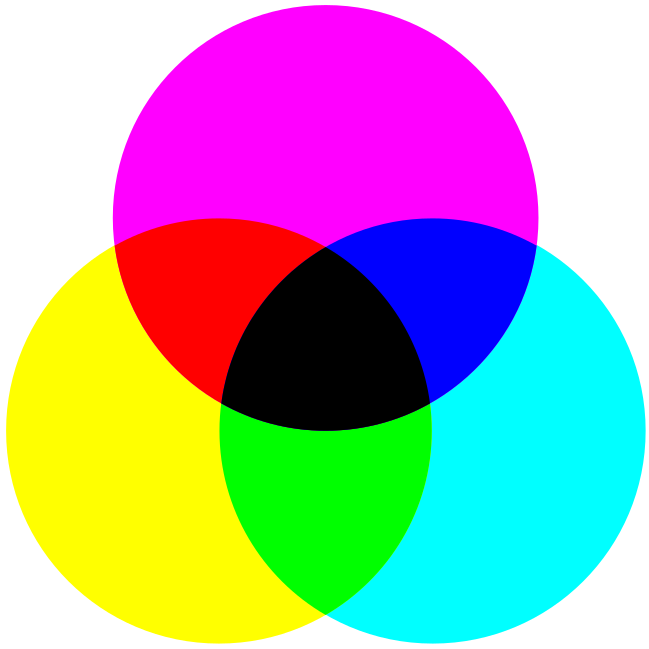
\includegraphics[width=0.5\textwidth]{bilder/farben-} 
% Bilddatei aus dem Unterverzeichnis bilder holen, skalieren auf 0.8*Satzspiegel
\caption {Die drei Grundfarben Cyan, Magenta und Gelb der subtraktiven Farbmischung ergeben zusammen schwarz (unbunt).\protect\footnotemark}\label{b_farben-}
\end{figure}

\footnotetext{\url{https://upload.wikimedia.org/wikipedia/commons/thumb/6/64/CMY_ideal_version_rotated.svg/649px-CMY_ideal_version_rotated.svg.png}}

\noindent Wenn man alle drei Grundfarben der subtraktiven Farbmischung mischt entsteht schwarz, weil dann alle Anteile im Licht abgezogen wurden.


\section{Hauttöne} \label{sec_hauttöne}
Von allen Farben nehmen die menschlichen Hauttöne eine besondere Rolle in dieser Arbeit ein, da die Auswirkung eines \glqq Red Tail\grqq\ bei der Personenbeleuchtung beobachtet werden soll. 2018 haben Herr Dr.-Ing. Trinh Quang Vinh und Herr Prof. Dr.-Ing. habil. Tran Quoc Khanh einen Artikel in der \glqq Licht\grqq\ über Licht und Hauttöne veröffentlicht. Sie haben unter anderem die spektralen Strahldichtefaktoren der Hauttöne von 15 Probanden untersucht. Dazu wurden die Hauttöne unter der Beleuchtung einer Halogenglühlampe mit kontinuierlichem Spektrum mit einem Strahldichtemessgerät gemessen\footnote{\cite[71]{vinhkhanh}} (Abbildung \ref{b_hautton}).
\begin{figure}[H]     % h=here, t=top, b=bottom, p=page
\centering
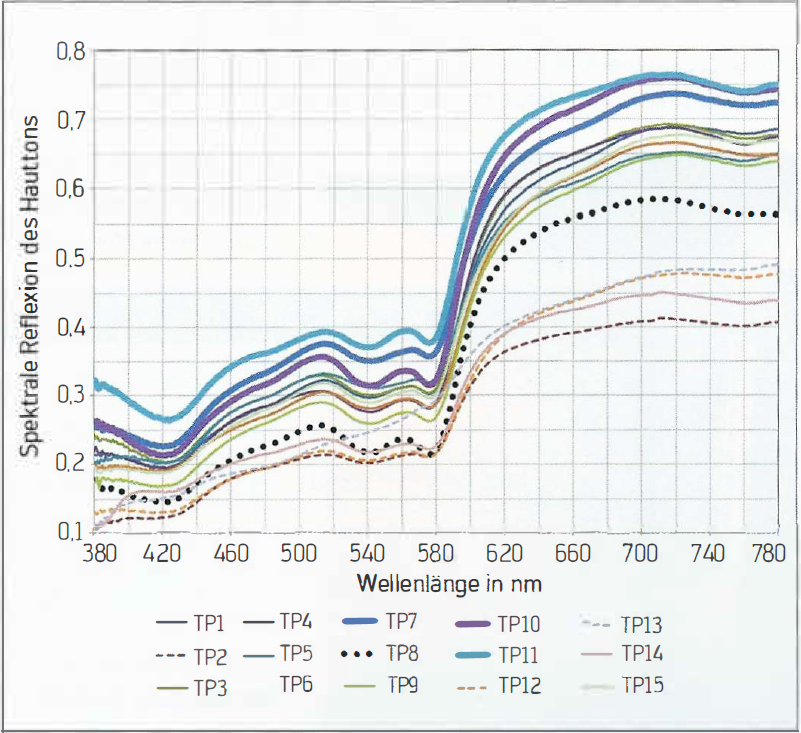
\includegraphics[width=0.8\textwidth]{bilder/hautton} 
% Bilddatei aus dem Unterverzeichnis bilder holen, skalieren auf 0.8*Satzspiegel
\caption {Spektrale Strahldichtefaktoren der 15 Hauttöne gemessen von Vinh und Khanh.\protect\footnotemark}\label{b_hautton}
\end{figure}

\footnotetext{\cite[71]{vinhkhanh}}

\noindent Aus diesem Graph lassen sich ein paar Schlussfolgerungen ableiten: Zum einen reflektieren Hauttöne am meisten den roten Spektralanteil des Lichts. Dies ist ein Hinweis darauf, dass ein zusätzlicher tiefroter Spektralanteil im Licht Hauttöne natürlicher aussehen lassen könnte. Zum anderen ist auch deutlich zu erkennen, dass Hauttöne alle Farben des Spektrums reflektieren und daher nicht nur Rot, sondern das gesamte Spektrum für die Personenbeleuchtung wichtig ist. Außerdem ist durch die unterschiedlichen Kurvenhöhen zu erkennen, dass bestimmte Hauttypen eine bestimmte Beleuchtung bevorzugen. Leider ist in dem veröffentlichten Artikel nicht angegeben, welche Hauttöne die verschiedenen Testpersonen hatten.

\chapter{Farbräume} 
In diesem Kapitel wird auf die Grundlagen der Farben und Farbräume eingegangen.
 
\section{RGB Farbraum} \label{sec_rgb}
Durch die Festlegung verschiedener Farbräume hat die  Internationale Beleuchtungskommission CIE (\glqq Commission Internationale de l'Eclairage\grqq) die Farben von Licht immer besser einordnen und beschreiben können. Der große Vorteil bei diesen Farbräumen besteht darin, dass man durch eine lineare Transformation von einer Farbraumdarstellung in die nächste Wechseln kann und die spektrale Empfindlichkeitskurve mit transformiert wird. So wird sichergestellt, dass jede Farbe nach der natürlichen Wahrnehmung des Menschen gewertet wird.
Angefangen hat all dies mit dem RGB-Farbraum. Dieser Farbraum wird mit den drei Grundfarben der additiven Farbmischung, den Primärvalenzen Rot, Grün und Blau aufgespannt. Die Farben ergeben jeweils die Ecken und in der Mitte entsteht so der Weißpunkt des Farbraumes. Eine Farbe lässt sich dann über die Farbkoordinaten r, g und b, die sich aus den Primärvalenzen errechnen, in diesem Farbraum orten\footnote{\cite[106]{hentschel}} (Gleichung \ref{gl_rgb1}).

\begin{equation}\label{gl_rgb1}
		r = \frac{R}{R+G+B},\quad g = \frac{G}{R+G+B},\quad b = \frac{B}{R+G+B}
\end{equation}
Der RGB-Farbraum ist so konstruiert, dass jede Kombination aus den drei Farbkoordinaten zusammen 1 ergibt. Es reichen also zwei Koordinaten aus, um den sogenannten Farbort bestimmen zu können, da sich die dritte Koordinate von selbst erschließt (Gleichung \ref{gl_rgb2}). 

\begin{equation}\label{gl_rgb2}
		b=1-r-g
\end{equation}
Der RGB-Farbraum kann auch dreidimensional als Würfel aufgespannent werden. Dort ist die Farbe schwarz der Ursprung und weiß die Kombination aus allen drei Farbvektoren (Abbildung \ref{b_rgb1}.

\begin{figure}[H]     % h=here, t=top, b=bottom, p=page
\centering
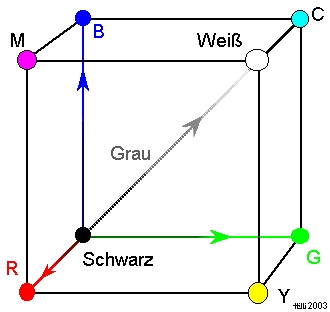
\includegraphics[width=0.5\textwidth]{bilder/rgb1} 
% Bilddatei aus dem Unterverzeichnis bilder holen, skalieren auf 0.8*Satzspiegel
\caption {Beim RGB-Würfel werden alle Primärvalenzen R, G, B als gleich lange Vektoren angenommen.\protect\footnotemark}\label{b_rgb1}
\end{figure}
\footnotetext{\url{http://www.hilli1.de/hillifarbe/Endlichfarbe/03122wf.jpg}}
 
\noindent Der RGB-Farbraum kann nicht alle Farben des sichtbaren Spektrum abbilden. W. D. Wright und J. Guild haben dazu Tests mit einem Monochromator gemacht. Ein Proband, der Farbflächen von $2^\circ$ Gesichtsfeldgröße sieht, sollte mit den Wellenlängen 700 nm (Rot), 546 nm (Grün) und 435 nm (Blau) die gesehene Farbe nachmischen (Abbildung \ref{b_rgb2}).

\begin{figure}[H]     % h=here, t=top, b=bottom, p=page
\centering
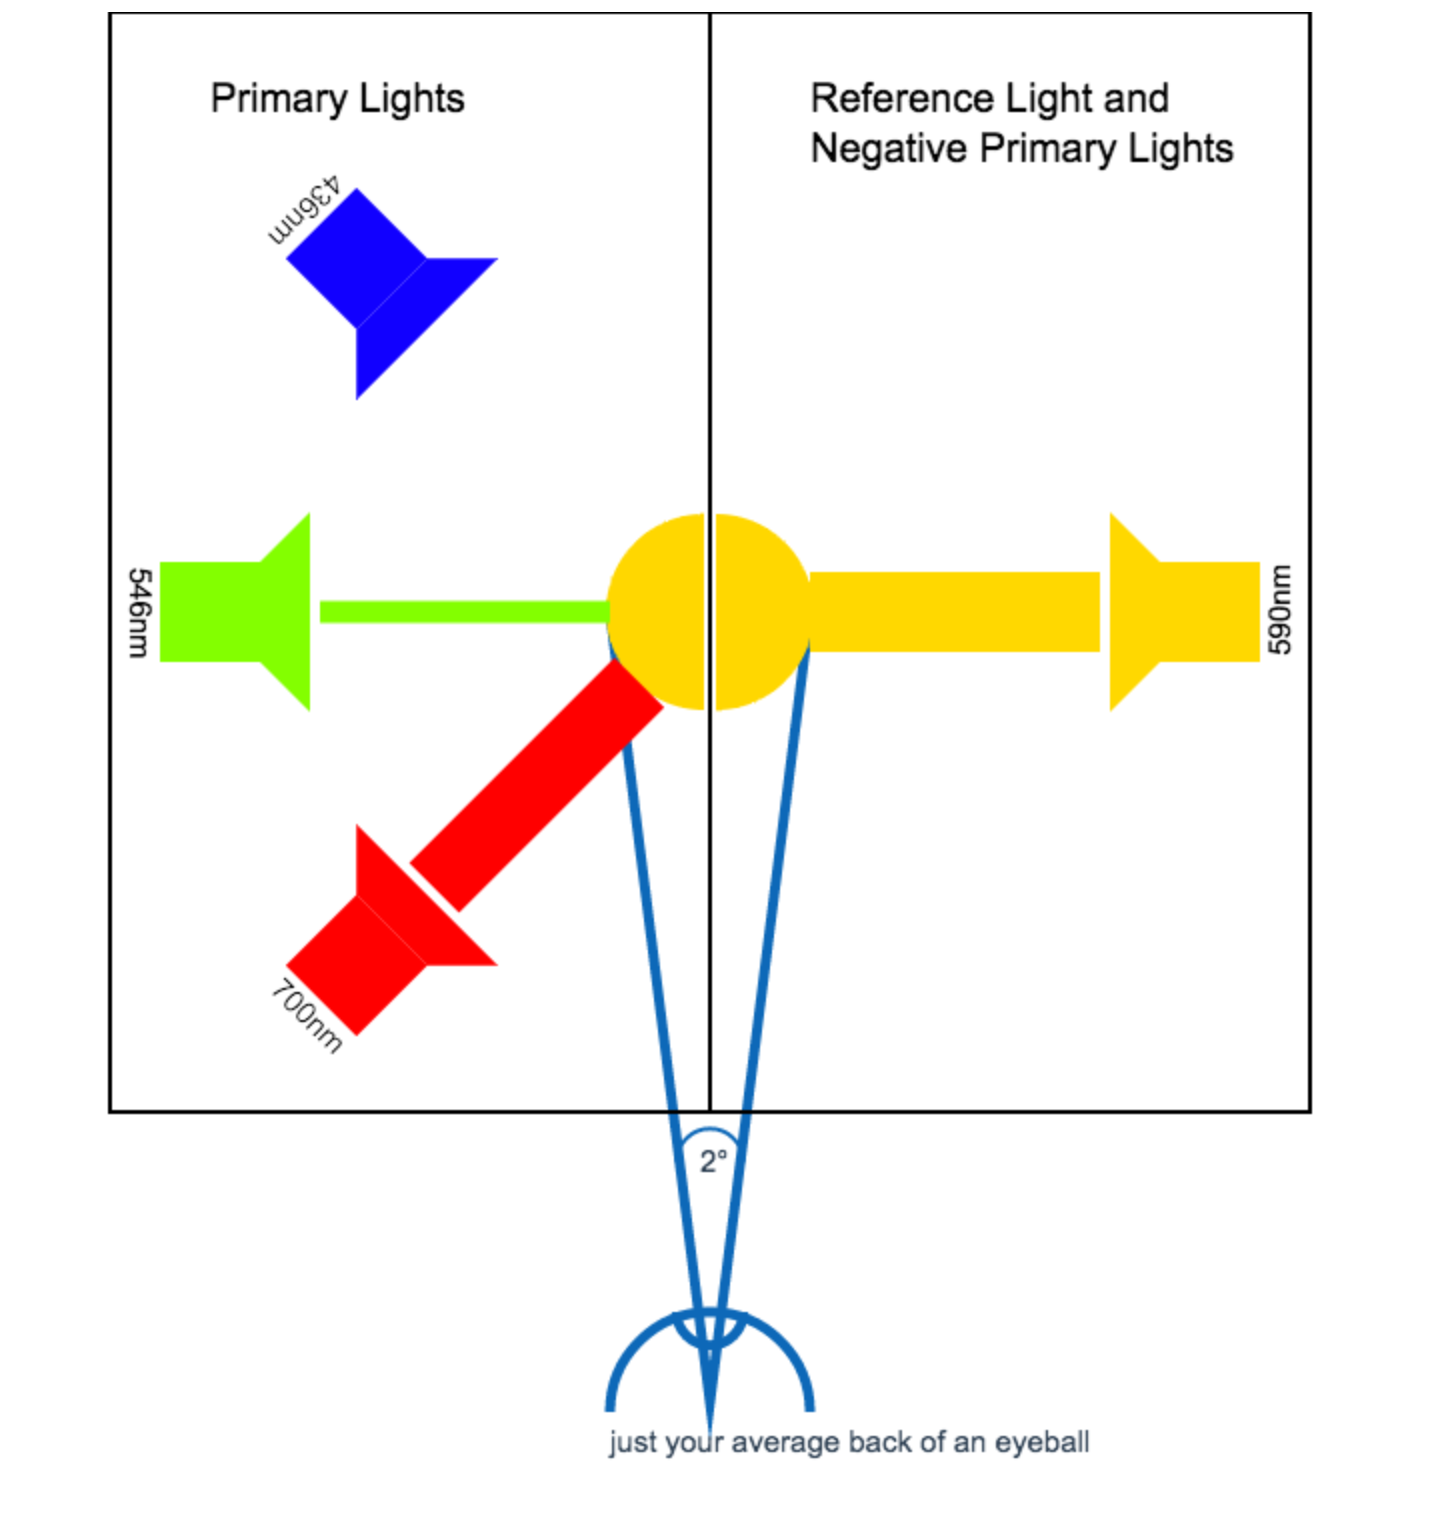
\includegraphics[width=0.8\textwidth]{bilder/rgb2} 
% Bilddatei aus dem Unterverzeichnis bilder holen, skalieren auf 0.8*Satzspiegel
\caption {Schematische Darstellung des Farbzuordnungsexperiments von Wright und Guild.\protect\footnotemark}\label{b_rgb2}
\end{figure}
\footnotetext{\url{https://cdn-images-1.medium.com/max/1600/0*75FcZwPv1Wu17_kc.png}}

\noindent Bei einer Referenzfarbe von zum Beispiel 500 nm (Blau-Grün) gab es keine Möglichkeit, diese Farbe mit den drei RGB-Farben zu mischen. Es musste sogar auf der Referenzfarbseite rot dazugemischt werden, damit man auf das Blau-Grün abgleichen konnte. Dies würde ein negativen Rot-Anteil im RGB-Farbraum bedeutet, den es so nicht geben kann. Daher hat die CIE 1931 ein virtuelles Primärvalenzssystem erarbeitet, dass alle sichtbaren Farben darstellen kann\footnote{\cite[77]{greule}}.\\

\section{CIE-XYZ Farbraum} \label{sec_xyz}
Im CIE-XYZ Farbraum gibt es die Primärvalenzen X, Y und Z, die aus einer linearen Transformation des RGB-Farbraum entstanden sind\footnote{\cite[76-77]{greule}} (Gleichungen  \ref{gl_xyz1} - 3.7).

\begin{eqnarray}\label{gl_xyz1}
		X = R_{x}\cdot R + G_{x}\cdot G + B_{x}\cdot B\\
		Y = R_{y}\cdot R + G_{y}\cdot G + B_{y}\cdot B\\
		Z = R_{z}\cdot R + G_{z}\cdot G + B_{z}\cdot B
\end{eqnarray}
Der Y-Wert entspricht dabei der Farbfunktion $y_{\lambda}$, die der $V(\lambda)$-Kurve (Abbildung \ref{b_augespek}) gleicht, und steht daher für die Helligkeit der Farbe. Dies ist eine Erweiterung zum RGB-Farbraum, in dem die Helligkeit nicht direkt mit einbezogen wurde. Der X-Wert zeigt den rot-grün-Anteil an und am Z-Wert lässt sich der Blau-Gelb-Anteil einer Farbe bestimmen\footnote{\cite[72]{mueller}} (Abbildung \ref{b_xyz2}).

\begin{figure}[H]     % h=here, t=top, b=bottom, p=page
\centering
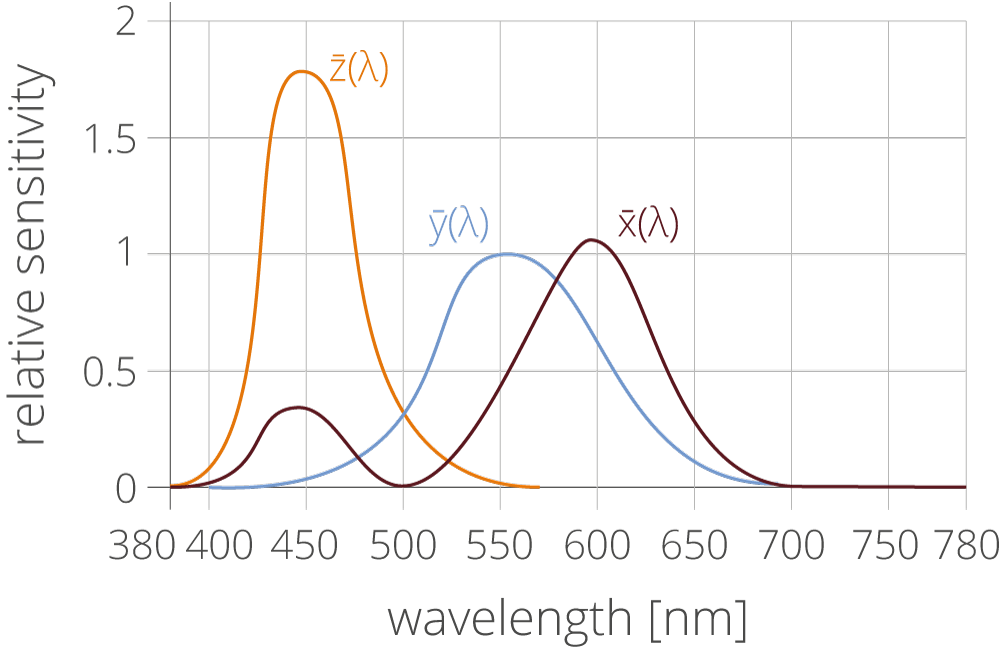
\includegraphics[width=0.8\textwidth]{bilder/xyz2} 
% Bilddatei aus dem Unterverzeichnis bilder holen, skalieren auf 0.8*Satzspiegel
\caption {Die XYZ-Spektralwertfunktionen, angepasst aus den r.\protect\footnotemark}\label{b_xyz2}
\end{figure}
\footnotetext{\url{https://www.gigahertz-optik.de/assets/Uploads/Abb.-II.21-neu.png}}
 
\noindent Aus diesen Primärvarlenzen lassen sie dich Farbanteile x, y und z ausrechnen, die auf der Farbtafel des CIE-XYZ Farbraums dargestellt werden (Gleichung \ref{gl_xyz2}). 

\begin{equation}\label{gl_xyz2}
		x = \frac{X}{X+Y+Z},\quad y = \frac{Y}{X+Y+Z},\quad z = 1-x-y
\end{equation}
Auch hier reichen zwei Normfarbwertanteile aus, um den Farbort (x,y) zu bestimmen. x steht für den Farbton und y für die Sättigung. Aus x und y kann jedoch kein Rückschluss auf die X, Y und Z Normalvalenzen gezogen werden und so ist zum Beispiel eine Bestimmung der Helligkeit (Y) aus dem Farbort nicht möglich\footnote{\cite[79]{greule}}.\\
Über die Grenzen des mit x und y aufgespannten Farbraums erstrecken sich von 380nm blau zu grün und gelb zu 780nm rot alle sichtbaren Farben des Spektrums. Die beiden Enden des Farbraumes sind auf der gegenüberliegenden Seite über die theoretische Purpur-Graden miteinander verbunden. Die Farben auf dieser Geraden werden vom menschlichen Auge magenta intertpretiert, gehören aber nicht mehr zum sichtbaren Wellenlängenbereich dazu\footnote{\cite[73]{mueller}}. Der Unbuntpunkt liegt bei $x=y=0,33$ (Abbildung \ref{b_xyz1}).

\begin{figure}[H]     % h=here, t=top, b=bottom, p=page
\centering
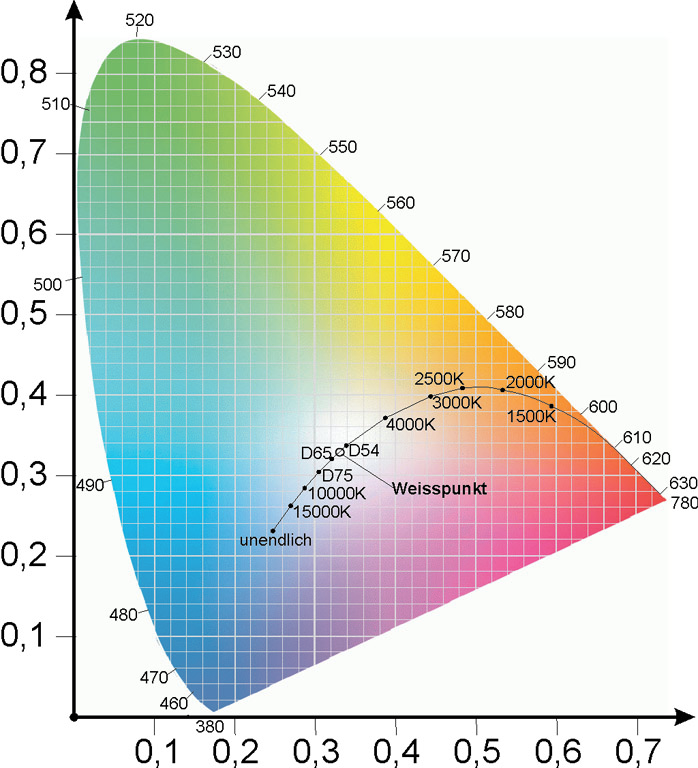
\includegraphics[width=0.7\textwidth]{bilder/xyz1} 
% Bilddatei aus dem Unterverzeichnis bilder holen, skalieren auf 0.8*Satzspiegel
\caption {Darstellung der CIE-XYZ Farbtafel eines $2^\circ$ Normalbeobachter.\protect\footnotemark}\label{b_xyz1}
\end{figure}

\footnotetext{\url{https://www.production-partner.de/wp-content/uploads/2018/02/Farbdreieck.jpg}}

\noindent Im XYZ-Farbdiagramm ist der Plank'sche Kurvenverlauf eingezeichnet. Wenn ein Farbort auf diese Kurve trifft wird ihm die jeweilige Farbtemperatur zugeschrieben. Landet der Farbort in der Nähe dieser Kurve wird der Farbe eine sogenannte korrelierte Farbtemperatur (correlated color temperature) zugesprochen. Es wurden damit die \glqq Geraden ähnlichster Farbtemperatur\grqq\ bestimmt, die anzeigen welche korrelierten Farbtemperatur vom Farbort getroffen wird (Abbildung \ref{b_cct})    

\begin{figure}[H]     % h=here, t=top, b=bottom, p=page
\centering
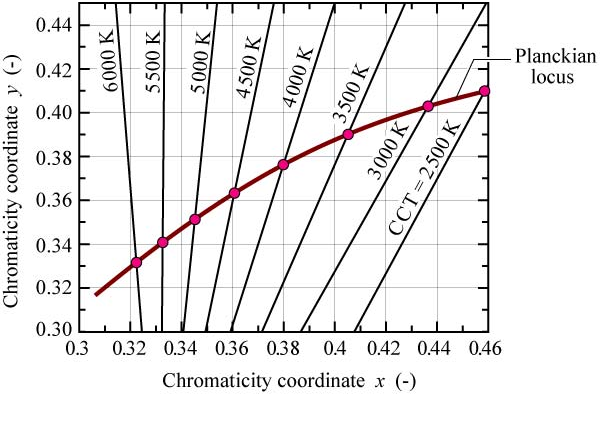
\includegraphics[width=0.8\textwidth]{bilder/cct} 
% Bilddatei aus dem Unterverzeichnis bilder holen, skalieren auf 0.8*Satzspiegel
\caption {Detailansicht des XYZ-Farbraumes mit den \glqq Geraden ähnlichster Farbtemperatur\grqq\ \protect\footnotemark}\label{b_cct}
\end{figure}

\footnotetext{\url{http://www.light.fi/blog/wp-content/uploads/2016/04/xyChromaticity-diagram.png}}

\noindent Trifft eine Leuchte mit ihren x, y Normfarbwertanteilen auf einen Punkt über der Plank'schen Kurve, so erscheint der Weißton grünstichig, trifft sie unter die Kurve, dann wirkt das Weiß magentastichig. Ist der Farbort zu weit von der Plank'schen Kurve entfernt, kann keine Farbtemperatur bestimmt werden.\\
Wenn man zwei Farben im XYZ-Farbraum vergleichen will, ist vorsichtig geboten, da die Farben auf der Farbtafel nicht mit gleich großem Abstand dargestellt werden. Dies ist daran zu erkennen, dass die Farbabstände im roten (620nm - 770nm) und blauen (380nm - 470nm) Bereich sehr nahe beieinander liegen, wohingehen sich der grüne Bereich(500nm - 570nm) sich über einen großen Anteil des hufeisenförmigen Rand erstreckt. Farbkontraste verhalten sich also nicht wie mit dem Auge wahrgenommenen Farben. Mit diesem Phänomen hat sich MacAdam beschäftigt und so sind 1940 die \glqq MacAdam Ellipsen\grqq\ entstanden (Abbildung \ref{b_ellipsen}).

\begin{figure}[H]     % h=here, t=top, b=bottom, p=page
\centering
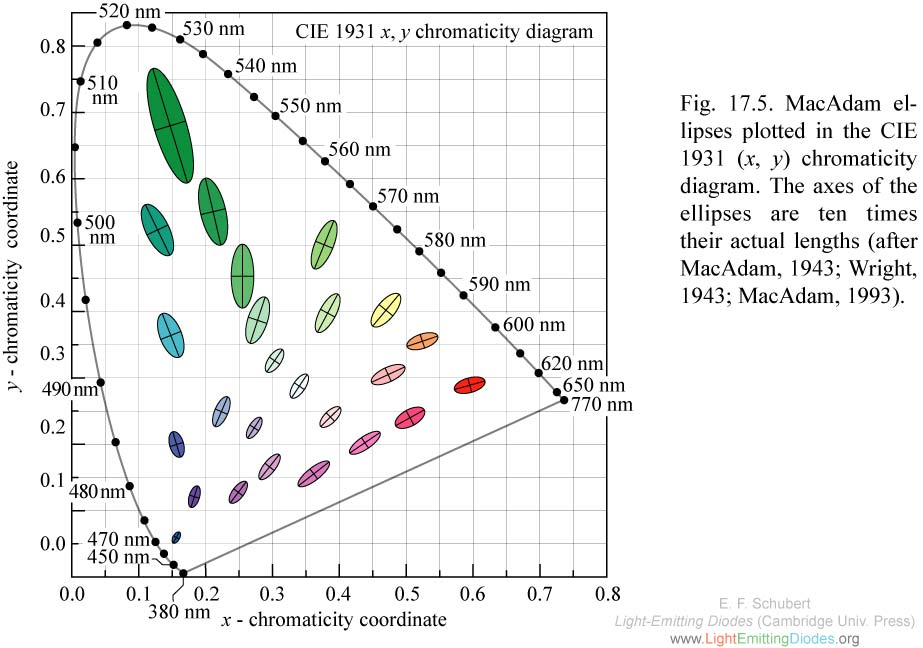
\includegraphics[width=1.0\textwidth]{bilder/ellipsen} 
% Bilddatei aus dem Unterverzeichnis bilder holen, skalieren auf 0.8*Satzspiegel
\caption {Abbildung der MacAdam Ellipsen im XYZ-Farbraum\protect\footnotemark}\label{b_ellipsen}
\end{figure}

\footnotetext{\url{https://ecse.rpi.edu/~schubert/Light-Emitting-Diodes-dot-org/chap17/F17-05\%20MacAdam\%20ellipses.jpg}}
\noindent Die MacAdam Ellipsen zeigen die Bereich an, in dem ein Normbalbeobachter zwei unterschiedliche Farborte dem selben Farbton zuordnen würde. Hätte der Farbraum annähernd gleiche Farbabstände, dann wären die Ellipsen kreisförmig.\\
Es wird also deutlich, dass der XYZ-Farbraum ein paar Schwächen aufweist. Das liegt daran, dass die X, Y und Z Primärvalenzen nur auf der additven Farbmischung beruhen. Die subtraktive Farbmischung, die ihr weiß aus 100\% Cyan, Magenta und Gelb mischt, ist in dieser Farbraumdarstellung nicht darstellbar (Farben  mit voller Sättigung liegen auf dem Kurvenrand). Außerdem hat MacAdam gezeigt, dass die Farbabstände nicht mit der realen Farbwahrnehmung zusammenhängt. So eignet sich der CIE-XYZ-Farbraum nur zur eindeutigen Bestimmung eines Farbreizes \footnote{\cite[79-80]{greule}}.


\section{CIE-unity chromity scale-Farbtafel (CIE-UCS)} \label{sec_ucs}
Damit die Farbabstände aus der Farbtafel besser mit der tatsächlichen Farbwahrnehmung übereinstimmt hat die CIE 1976 die UCS-Farbtafel definiert. Für diese Farbtafel werden die x und y Normfarbwertanteile so transformiert, dass die Farbabstände vereinheitlicht sind (Gleichgung \ref{gl_ucs1}).

\begin{equation}\label{gl_ucs1}
		u' = \frac{4x}{-2x+12y+3} \quad v' = \frac{9y}{-2x+12y+3}
\end{equation}
Es wurden also die Farbbereiche aneinander angeglichen und die Farbtafel hat sich gedreht. Dadurch ähneln die Farbabständen den real empfunden Abständen schon deutlich besser als im XYZ-Farbraum. Durch die Transformation sind auch die MacAdam Ellipsen deutlich kreisförmiger geworden (Abbildung \ref{b_ucs}).  

\begin{figure}[H]     % h=here, t=top, b=bottom, p=page
\centering
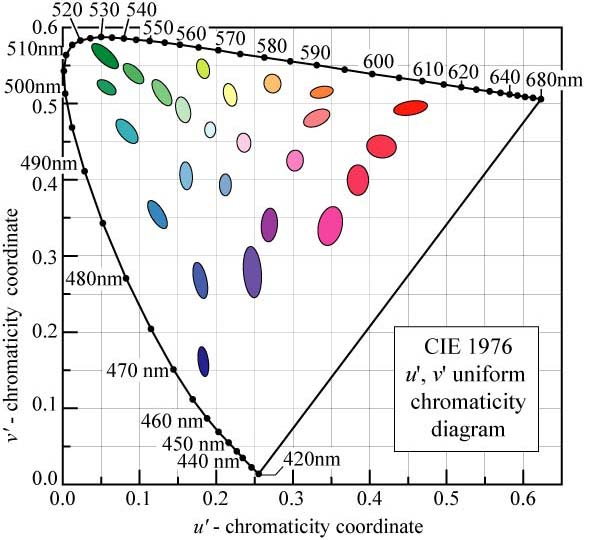
\includegraphics[width=0.8\textwidth]{bilder/ucs} 
% Bilddatei aus dem Unterverzeichnis bilder holen, skalieren auf 0.8*Satzspiegel
\caption {Abbildung der MacAdam Ellipsen auf der UCS-Farbtafel \protect\footnotemark}\label{b_ucs}
\end{figure}

\footnotetext{\url{https://www.fktg.org/sites/default/files/sauter_bild_02.jpg}}

\noindent Durch die CIE-UCS Farbtafel ist auch der $\Delta$u'v' entstanden. Dieser Wert ist wie beim TLCI (Kapitel \ref{sec_tlci}) ein Maß dafür, wie weit ein $u'_{i}$, $v'_{i}$ - Farbort mit korrelierter Farbtemperatur x von dem Plank'schen Kurvenzug bei Farbtemperatur x ($u'_{0}$, $v'_{0}$) entfernt ist\footnote{\cite[566]{jiyupe}} (Abbildung \ref{b_duv}).

\begin{figure}[H]     % h=here, t=top, b=bottom, p=page
\centering
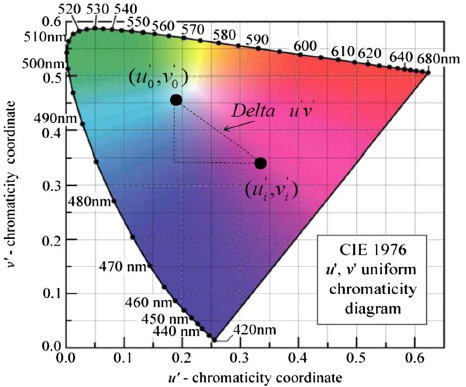
\includegraphics[width=0.8\textwidth]{bilder/duv1} 
% Bilddatei aus dem Unterverzeichnis bilder holen, skalieren auf 0.8*Satzspiegel
\caption {Darstellung des $\Delta$u'v' auf der UCS-Farbtafel}\label{b_duv}
\end{figure}


\noindent Anhand des Wertes ist erkennbar, ob das gemischte Weiß grünstichig mit $\Delta u'v' < 0$ oder magentastichtig mit $\Delta u'v' > 0$ ist (Gleichung \ref{gl_duv1}).

\begin{equation}\label{gl_duv1}
		\Delta u'v'=\sqrt{(du')^{2}+(dv')^{2}}=\sqrt{(u'_{i}-u'_{0})^{2}+(v'_{i}-v'_{0})^{2}}
\end{equation}
Dieser Wert wird zur Einschätzung der Weißlichtqualität in Kombination mit einem Farbwiedergabewert zur Rate gezogen und ist daher auch bei den \glqq Red Tail\grqq\ -Messung von größerer Bedeutung. Eine Abweichung von $\Delta u'v' < \pm 0.005$ ist für ein gutes weiß akzeptabel\footnote{\cite{ohno}}.\\
Auf der UCS-Farbtafel lassen sich nur Farben gleicher Helligkeit miteinander vergleichen. Um Farben verschiedener Helligkeiten vergleichen zu können hat die CIE noch weitere dreidimensionale Farbräume bestimmt, die für die Red-Tail-Untersuchungen, aber keine größere Rolle spielen.\newpage


\chapter{Farbwiedergabewerte}
Es gibt mehr als vierzig verschiedene Methoden, um die Farbwiedergabe einer Leuchte zu beurteilen. In diesem Kapitel sollen die in der Medien- und TV-Branche typischen Farbwiedergabeindices vorgestellt und deren Relevanz für die Messung mit dem \glqq Red Tail\grqq\  aufgezeigt werden.

\section{CIE: Color Rendering Index (CRI)} \label{sec_cri}
Da der Farbort allein keine eindeutige Aussage über die Zusammensetzung des Spektrums zulässt, wurde 1965 von der Internationalen Beleuchtungskommission ein Testverfahren entwickelt, mit dem die Farbwiedergabe (Color Rendering Index) einer Leuchte bestimmt werden kann. Dafür werden acht Referenzfarben festgelegt. Bei einer CRI-Messung wird also überprüft, wie gut eine Lichtquelle diese Körperfarben wiedergeben kann. Es wird dabei zwischen einem schwarzen Strahler(< 5000K) und Tageslicht(> 5000K) differenziert. Die gemessenen Unterschiede zu den Referenzfarben($R_{1}$-$R_{8}$) werden mit Werten von 0 bis 100 gewichtet, wobei ein Wert von 100 aussagt, dass die Farbe bestmöglich wiedergegeben wird. Bei der Berechnung des CRI werden zuerst einzelnene Indexwerte $R_{i}$ der Farben i aus den Farbdifferenzen $\Delta E_{i}$ berechnet (Gleichung \ref{gl_cri1})\footnote{\cite{davis_ohno}}.
	\begin{equation}\label{gl_cri1}
		R_{i} = 100 - 4,6 \cdot \Delta E_{i}
	\end{equation}
Die Farbdifferenzen $\Delta E_{i}$ werden mit 4,6 skaliert, damit die CIE Normlichtart F4 einen daraus berechneten $R_{a}$-Wert von 51 bekommt. Die Normlichtart F4 ist mit ihrem Spektrum repräsentativ für eine damalige  Standartleuchtstofflampe. Weil mit dem CRI häufig Aussagen über Leuchtstofflampen gemacht werden, wird die Normlichtart F4 als Referenz in die Mitte der Farbwiedergabeskala geschoben.\footnote{\cite{housmoss}}\\
Damit der CRI berechnet werden kann, werden diese acht Werte  schließlich arithmetisch gemittelt und es ergibt sich der Gesamtwert $R_{a}$,  welcher repräsentativ für die Farbwiedergabe der Leuchte steht (Gleichung \ref{gl_cri2})\footnote{\cite{production partner}}.
	\begin{equation}\label{gl_cri2}
		R_{a} =\frac{1}{8} \sum_{i=1}^{8} R_{i}
	\end{equation}
In der DIN 6169 werden zur besseren Beurteilung der Farbwiedergabe die $R_{a}$-Werte in verschiedene Stufen unterteilt (Tabelle \ref{t_cri}).

	\begin{table}[htp] 
		\rowcolors{1}{}{lgray} 
		\centering
		\begin{tabular}{rlcc}  % Spalten nach Ausrichtung: l, c, r, p{breite} 
		\toprule
		\multicolumn{3}{c}{\large\sffamily Stufen des CRI}\\ 							
		\midrule
		1A & $R_{a} \geq 90$ & sehr hohe Anforderung\\ 
		1B & 90 > $R_{a} \geq 80$ & sehr hohe Anforderung\\
		2A & 80 > $R_{a} \geq 70$ & hohe Anforderung\\
		2B & 70 > $R_{a} \geq 60$ & hohe Anforderung\\
		3 & 60 > $R_{a} \geq 40$ & mittlere Anforderung\\
		4 & 40 > $R_{a} \geq 20$ & geringe Anforderung\\
		\bottomrule
		\end{tabular}
		\caption{$R_{a}$ eingeteilt in verschiedene Stufen\protect\footnotemark}	
		\label{t_cri}
	\end{table}
	\footnotetext{\cite[111]{hentschel}}

\noindent Ein hoher $R_{a}$-Wert beschreibt aber nur bedingt die Farbwiedergabe einer Leuchte, da beispielsweise keine Angabe über die Sättigung der Farben gemacht wird, weil die acht Referenzfarben nur Pastelltöne sind. Da der CRI damals für Glühlicht entwickelt wurde. Gesättigte Farben fließen nicht in die Bewertung mit ein.
Das wirkt sich auch auf die Vergleichbarkeit von Leuchten aus. Zwei Scheinwerfer mit demselben $R_{a}$-Wert von 90 können sehr unterschiedliche Spektren haben und damit sehr unterschiedlich Farben darstellen, trotz gleichem Farbwiedergabeindex.
Außerdem kann nur schwer eine Aussage darüber gemacht werden, ob sich eine Leuchte mit einem guten CRI für Personenbeleuchtung eignet, weil Rottöne und Hauttöne in diesem Bewertungsverfahren fehlen.\\\\
Leuchtstofflampen nutzten den CRI aus, indem durch gezielte schmalbandige Peaks im Spektrum die Referenzfarben getroffen werden. Auf diese Weise kann zwar ein hoher CRI-Werte erreicht werden, aber kein breitbandiges und ausgefülltes Lichtspektrum entstehen. Zusätzlich entsteht bei LED-Leuchtmitteln ein ähnliches Problem, wie bei den Leuchstoffröhren. Man kann das Spektrum mit den Peaks gut auf die Referenzfarben ausrichten, ohne das Gesamte Spektrum abdecken zu müssen. Gerade bei LED-Leuchten kann dieses Verhalten des CRI ausgenutzt werden, um kritische Bereiche zu verschleiern. Daher sah sich die CIE gezwungen den Farbwiedergabeindex zu erweitern. In dem neueren $R_{e}$-Wert gibt es nun auch gesättigte Farben und eine Hautfarbe wird miteinbezogen (Abb. \ref{b_cri}).

\begin{figure}[H]     % h=here, t=top, b=bottom, p=page
\centering
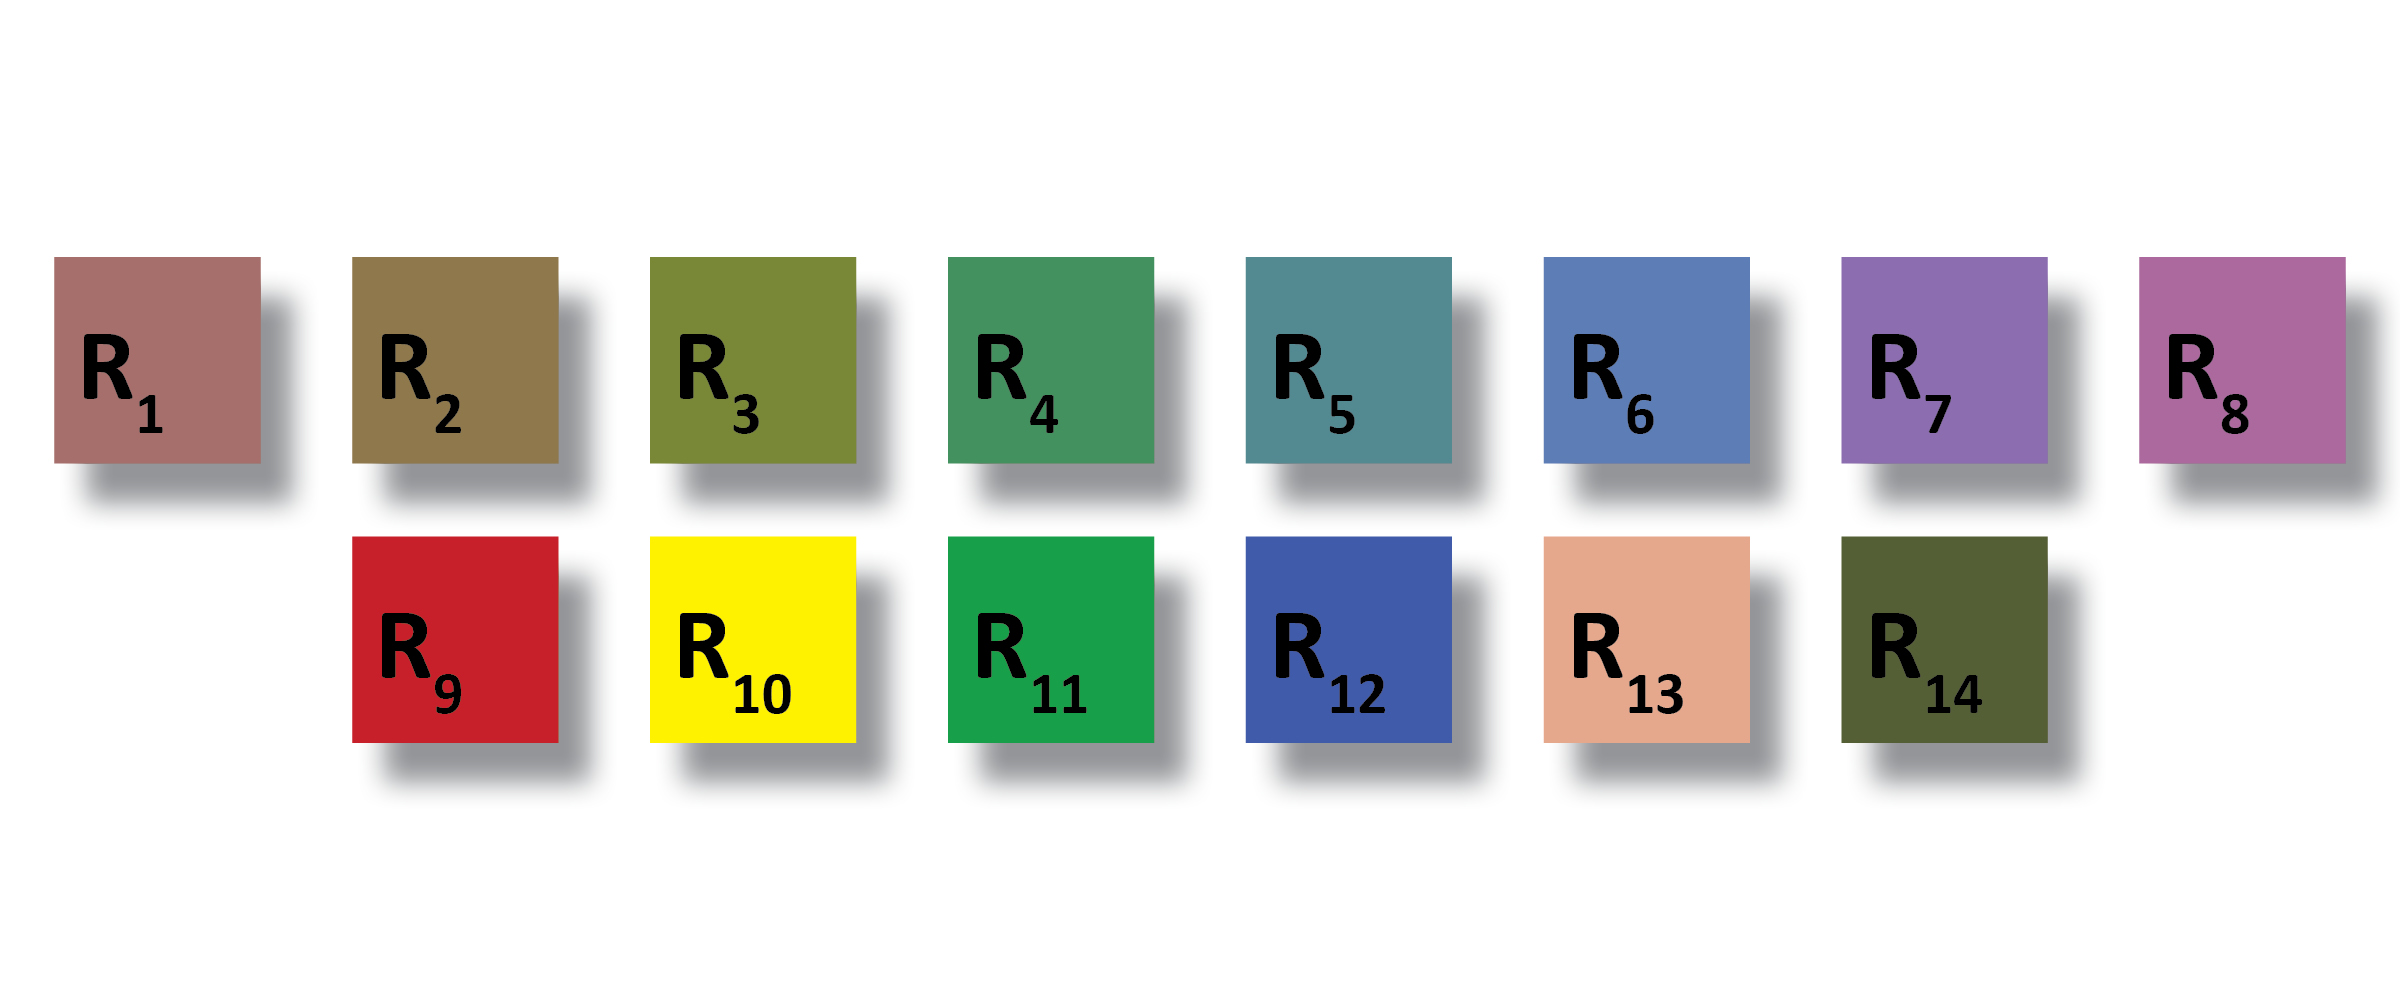
\includegraphics[width=0.8\textwidth]{bilder/cri} 
% Bilddatei aus dem Unterverzeichnis bilder holen, skalieren auf 0.8*Satzspiegel
\caption {Alle Referenzfarben des Farbwiedergabeindexes: $R_{1}$ Altrosa, $R_{2}$ Senfgelb, $R_{3}$ Gelbgrün, $R_{4}$ Hellgrün, $R_{5}$ Türkisblau, $R_{6}$ Himmelblau, $R_{7}$ Asterviolett, $R_{8}$ Fliederviolett, $R_{9}$ Rot gesättigt, $R_{10}$ Gelb gesättigt, $R_{11}$ Grün gesättigt, $R_{12}$ Blau gesättigt und $R_{13}$ Rosa (Hautfarbe), $R_{14}$ Blattgrün \protect\footnotemark}\label{b_cri}
\end{figure}

\footnotetext{\url{https://www.elementalled.com/wp/wp-content/uploads/2015/08/CRI_chart.jpg}}

\noindent Aus dem Demofile der JETI\glqq LiVal\grqq -Software kann bei einer warmweißen LED ein CRI von 82 bestimmt werden (Abbildung \ref{b_cri2}). Der $R_{e}$-Wert ist naturgemäß schlechter als der $R_{a}$-Wert. Mit 77 ist dieser noch akzeptabel, da der $R_{9}$-Wert (gesättigtes Rot) nur 15 Punkte erbringt. Diese Leuchte entspricht \glqq sehr hohen Anforderungen\grqq\ (Tabelle \ref{t_cri}) und ist damit nach Definition sehr gut in der Farbwiedergabe. Solche einzelne schlechte Referenzwerte werden durch die arithmetische Mittlung der Referenzfarbwerte begünstigt.Sie mindern den $R_{a}$-Wert nicht beträchtlich. Beispielsweise wird bei Weißen-LEDs der fehlende Rotanteil nur am niedrigen $R_{9}$-Wert sichtbar, aber im CRI-Wert sind diese Schwächen einer LED-Leuchte kaum erkennbar\footnote{\cite{davis_ohno}}. 

\begin{figure}[htp]     % h=here, t=top, b=bottom, p=page
\centering
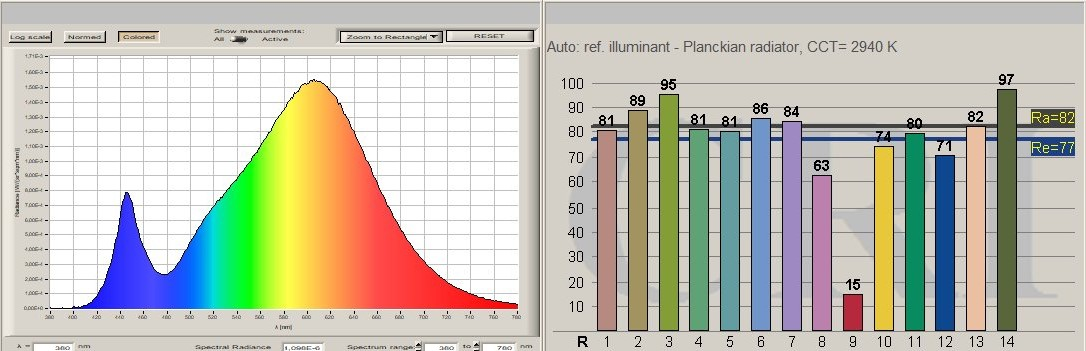
\includegraphics[width=1.0\textwidth]{bilder/cri2} 
% Bilddatei aus dem Unterverzeichnis bilder holen, skalieren auf 0.8*Satzspiegel
\caption {Messung einer warmweißen LED-Leuchte (Ausschnitt aus dem Demofile des Programmes \glqq LiVal\grqq\ von der Firma JETI): Links ist das Lichtspektrum der Leuchte dargestellt, rechts die gemessenen CRI-Werte  \protect\footnotemark}\label{b_cri2}
\end{figure}
\noindent Der CRI kann daher eher als richtungsweisend betrachtet werden: Eine Leuchte mit guter Farbwiedergabe wird auch immer einen guten CRI-Wert haben. 
Zum Vergleich für Leuchten eignen sich andere Farbwiedergabewerte heutzutage besser\footnote{\cite{production partner}}.\\\\
Aus diesen Gründen und der Erkenntnis der CIE, \emph{\glqq dass die CRI-Methode generell nicht anwendbar ist, um eine Anzahl von Lichtquellen gemäß ihrer Farbwiedergabe einzuordnen, wenn weiße LEDs darunter sind\grqq}\ \citep[VI]{CIE}, wird sich diese Arbeit hauptsächlich auf andere Farbwiedergabewerte konzentrieren. Der CRI wird aber mit aufgeführt, weil dieser in der Scheinwerfer- und Fernsehbranche (noch) einen hohen Stellenwert inne hat.



\section{NIST: Color Quality Scale (CQS)} \label{sec_cqs}

Der Color Quality Scale, der von dem National Institute of Standards and Technology (NIST) erarbeitet wurde, orientiert sich an der Grundidee des CRI und versucht dessen Probleme anzugehen sowie ihn zu ersetzen. So gibt es fünfzehn vollständig saturierte Referenzfarben, die auch auf LED-Leuchten anwendbar sind. Über Skaleneffekte soll der CQS auch indirekt eine Aussage über die Farbwiedergabe von Pastelltönen ermöglichen (Abb. \ref{b_cqs1}). 

\begin{figure}[htp]     % h=here, t=top, b=bottom, p=page
\centering

\includegraphics[width=0.8\textwidth]{bilder/cqs} 
% Bilddatei aus dem Unterverzeichnis bilder holen, skalieren auf 0.8*Satzspiegel
\caption {Alle Referenzfarben des CQS mit voller Sättigung\protect\footnotemark}\label{b_cqs1}
\end{figure}

\footnotetext{\url{https://www.lemoledlight.com/wp-content/uploads/2016/04/LED-Lighting-CRI-5.jpg}}
\noindent Der CQS wertet eine Übersättigung der Farbe nicht, nur eine Abweichung von Farbton oder Helligkeit wird bestraft. Dies steht im Gegensatz zum CRI, bei dem weniger Punkte für eine Farbe vergeben wird, wenn diese übersättigt wurde, also die Leuchte eine höhere Farbigkeit hatte als das Referenzlicht des CRI. Wenn beispielsweise eine Oberfläche eines Objekts beleuchtet wird, kann eine übersättigte Farbe jedoch gewünscht sein und ist daher nicht pauschal negativ einzuordnen\footnote{\cite[3]{davis_ohno}}.\\
Durch die Art der Berechnung der CQS-Wertes ist an diesem deutlicher zu erkennen, ob ein Leuchtmittel eine eher gute oder eher schlechte Farbwiedergabe aufweist. 
Der CQS-Wert lässt sich mit Hilfe von drei Formeln berechnen. Dazu wird zuerst der Farbdifferenzwert $\Delta E_{rms}$ aus dem quadratischen Mittel (root-mean-square) der 15 Farbunterschiede $\Delta E_{i}$ berechnet\footnote{\cite[5]{davis_ohno}}: 

\begin{equation}\label{gl_cqs1}
		\Delta E_{rms} = \sqrt{\frac{1}{15} \sum_{i=1}^{15} \Delta E_{i} ^{2}} 
\end{equation}
Aus diesem Farbdifferenzwert wird ähnlich wie beim CRI (Gleichung \ref{gl_cri1}) ein Farbwiedergabewert $Q_{f,rms}$ errechnet (Gleichung \ref{gl_cqs2}).

\begin{equation}\label{gl_cqs2}
		Q_{f,rms} = 100 - 3,0305 \cdot \Delta E_{rms} 
\end{equation}
Schließlich wird durch eine Skalierung auf Werte von 0 bis 100 aus diesem Farbwiedergabewert der CQS-Wert $Q_{f}$  (Gleichung \ref{gl_cqs3}). Dadurch entfallen beim CQS negative Farbwerte, die beim CRI sehr schwierig zu interpretieren sind. 

\begin{equation}\label{gl_cqs3}
		Q_{f} = 10 \ln(e^{\frac{Q_{f,rms}}{10}}+1) 
\end{equation}\\
Der CQS wird mit seinen fünfzehn Referenzfarben im CIELAB-Farbraum eingezeichnet. Da die Abstände von Farborten in diesem Farbraum in etwa wahrgenommenen Farbunterschieden entsprechen, kann gut erkannt werden, wie stark sich die Farbwiedergabe einer Leuchte den Referenzwerten ähneln(Abb. \ref{b_cqs2a} und \ref{b_cqs2b}).\\

\begin{figure}[H]     % h=here, t=top, b=bottom, p=page
\centering
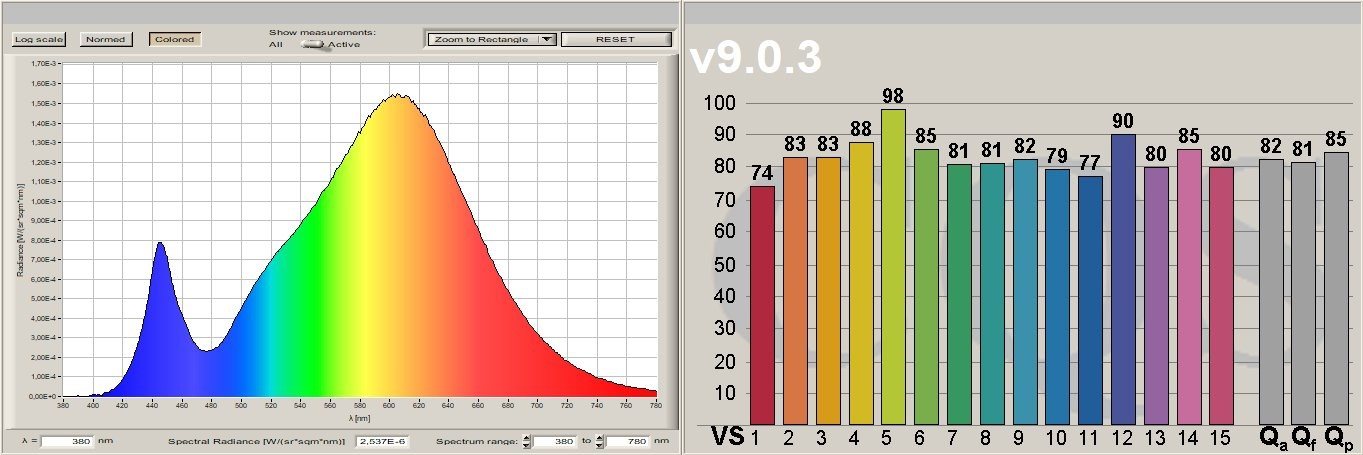
\includegraphics[width=0.9\textwidth]{bilder/cqs2a} 
% Bilddatei aus dem Unterverzeichnis bilder holen, skalieren auf 0.8*Satzspiegel
\caption {Ausschnitt aus dem Programm \glqq LiVal\grqq\ von der Firma JETI: Demo Spektrum einer warmweißen LED (2942K) mit $Q_{f} = 81$}\label{b_cqs2a}
\end{figure}

\begin{figure}[H]     % h=here, t=top, b=bottom, p=page
\centering
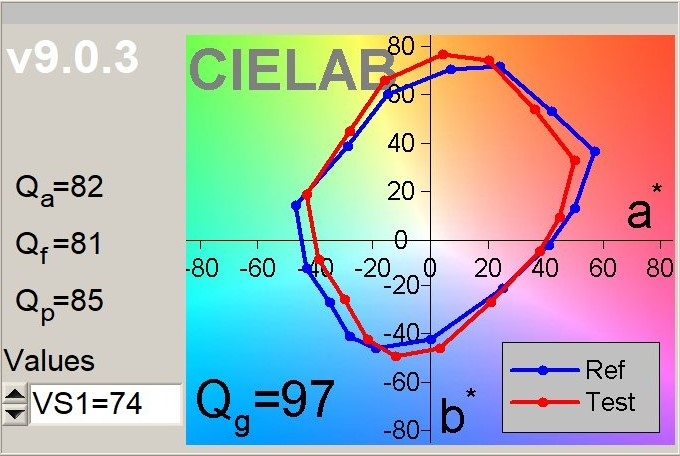
\includegraphics[width=0.7\textwidth]{bilder/cqs2b} 
% Bilddatei aus dem Unterverzeichnis bilder holen, skalieren auf 0.8*Satzspiegel
\caption {Ausschnitt aus dem Programm \glqq LiVal\grqq\ von der Firma JETI: Die fünfzehn Referenzfarben(blau) im CIELAB-Farbraum im Vergleich zu den gemessenen Werten (rot)}\label{b_cqs2b}
\end{figure}

\noindent Auf die in den Abbildung \ref{b_cqs2a} und \ref{b_cqs2b} erwähnten Werte $Q_{a}$ (optimierter CQS-Wert für kaum übersättigte Farben), $Q_{p}$ (optimierter CQS-Wert für viele übersättigte Farben) und $Q_{g}$(optimierter CQS-Wert im Zusammenhang mit dem Gamut Area Index) wird in dieser Arbeit nicht weiter eingegangen, weil sie über den Rahmen dieser Bachelorarbeit hinaus gehen und nicht relevant für diese Thesis sind\footnote{\cite[60-62]{khanh}}. \\
Da der CQS ähnlich wenige Referenzfarben nutzt wie der CRI und keine besondere Aussage über die Farbwiedergabe von Hauttönen im TV-Bereich liefert, wird bei den Messungen dieser Arbeit das Hauptaugenmerk nicht auf dem CQS liegen. Der CQS eignet sich besser zur Einschätzung der Farbwiedergabe ohne Bezug zu einer TV-Kamera. 


\newpage 
\section{EBU: Television Lighting Consistency Index (TLCI)} \label{sec_tlci}
Die European Broadcast Union (EBU) hat 2012 einen neuen lichttechnischen Parameter bestimmt, der auf den Film- und Fernsehbereich zugeschnitten ist, den Television Lighting Consistency Index, um einen Zusammenhang zwischen Farbwiedergabewert und Kamera zu schaffen.
Wie eine Messung des TLCI vonstattengeht ist in diesem Blockschaltbild der EBU verdeutlicht (\ref{b_tlci1}):

\begin{figure}[htp]     % h=here, t=top, b=bottom, p=page
\centering
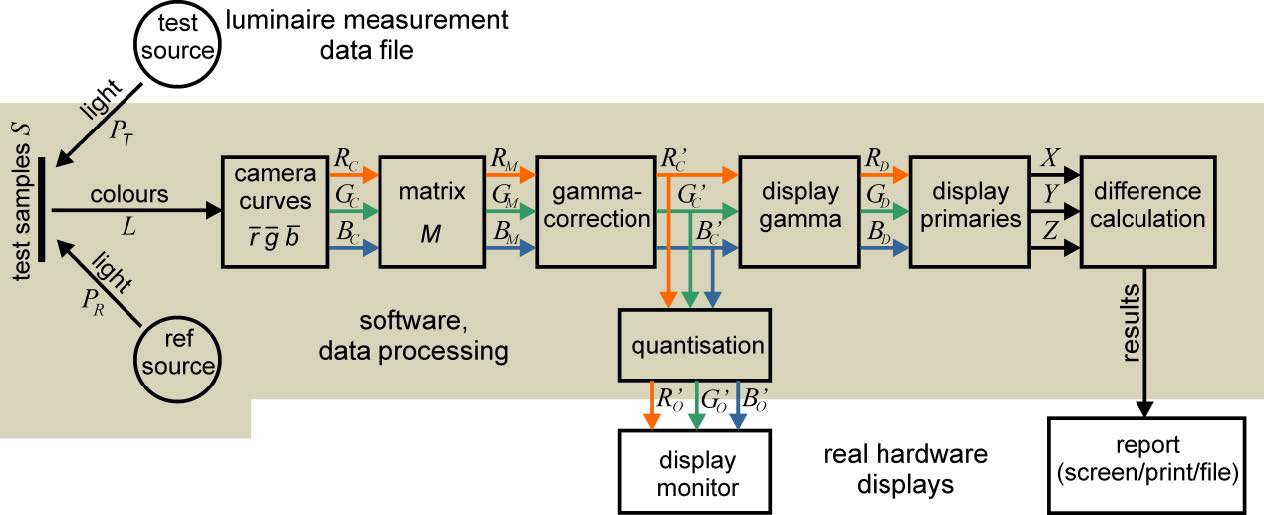
\includegraphics[width=1.0\textwidth]{bilder/tlci1} 
% Bilddatei aus dem Unterverzeichnis bilder holen, skalieren auf 0.8*Satzspiegel
\caption {Blockschaltbild einer TLCI-Wertbestimmung \protect\footnotemark}\label{b_tlci1}
\end{figure}
\footnotetext{\cite[15]{roberts}}
\noindent Zur Ermittlung des TLCI wird eine Testtafel mit 24 Farben von einer \glqq Standartkamera\grqq\ gefilmt. Die von der Kamera gefilmten Farben werden dann in einem Datenfile gespeichert. Diese Daten werden analysiert, um die Farbtemperatur zu bestimmen und so die Referenzdaten zu erstellen. Anschließend wird diese Tafel von der zu testenden Leuchte bestrahlt und ebenfalls gefilmt. Auf einem an die Kamera angeschlossenen \glqq Standartbildschirm\grqq\ werden die TLCI-Messergebnisse angezeigt. Die Kamera gewichtet die reflektierten Farben mit ihren $\bar{r}$-, $\bar{g}$- und $\bar{b}$-Kamerakurven und die Farbtemperatur wird bestimmt\footnote{\cite[16]{roberts}} (Gleichung \ref{gl_tlci05}).
\begin{equation}\label{gl_tlci05}
R_{C}=\sum_{\lambda=380}^{760} R_{\lambda} \cdot P_{\lambda} \cdot \bar{r}_{\lambda} \qquad G_{C}=\sum_{\lambda=380}^{760} R_{\lambda} \cdot P_{\lambda} \cdot \bar{g}_{\lambda} \qquad B_{C}=\sum_{\lambda=380}^{760} R_{\lambda} \cdot P_{\lambda} \cdot \bar{b}_{\lambda}
\end{equation}
Dabei entspricht $\lambda$ der Wellenlänge, $R_{\lambda}$ der Reflektion der Testfarbe und $P_{\lambda}$ der spektralen Verteilung des Lichts der Test bzw. Referenzleuchte.
\newpage
\noindent Die so entstandenen $R_{C}$, $G_{C}$ und $B_{C}$-Werte werden dann im zweiten Schritt auf weiß abgeglichen (Kapitel \ref{sec_wb}). Diese Weißabgleichswerte $R_{Cb}$, $G_{Cb}$ und $B_{Cb}$ werden mit einer linearen Matrix M bewertet, um die Werte des RGB-Signals zu erhalten\footnote{\cite[16]{roberts}} (Gleichung \ref{b_tlci1}).
\begin{equation}\label{gl_tlci1}
\begin{bmatrix} R \\ G \\ B \end{bmatrix}= 
\begin{bmatrix} 1,182 & -0,209 & 0,027 \\ 0,107 & 0,890 & 0,003 \\ 0,004 & -0,134 & 1,094 \end{bmatrix}
\begin{bmatrix} R_{Cb} \\ G_{Cb} \\ B_{Cb} \end{bmatrix}
\end{equation}\\
Die RGB-Werte werden in einer zweiten Matrix verrechnet, damit die Sättigungswerte der Farben übereinstimmen (Empfehlung der EBU: 90 \% Sättigung). Im nächsten Schritt werden die eben berechneten $R_{M}$, $G_{M}$ und $B_{M}$-Werte der einzelnen Farben von der Gammakurve der Kamera vorverzerrt (Kapitel \ref{sec_gamma}).
Beim Bildschirm angekommen werden die R'G'B'-Werte der Farben mit der Gammakurve des Bildschirm wieder entzerrt (Empfehlung der EBU: $\gamma$ = 2,4)\footnotetext{\cite[21]{roberts}}. Für die 24 Farben der Testtafel werden dann im vorletzten Schritt mit der XYZ()-Matrix die Farbkoordinaten X, Y und Z für den Bildschirm aus den Gamma entzerrten Werten  $R_{d}$, $G_{d}$ und $B_{d}$ errechnet\footnote{\cite[17]{roberts}} (Gleichung \ref{b_tlci2}).
\begin{equation}\label{gl_tlci2}
\begin{bmatrix} X \\ Y \\ Z \end{bmatrix}= 
\begin{bmatrix} XYZ(0,0) & XYZ(0,1) & XYZ(0,2) \\ XYZ(1,0) & XYZ(1,1) & XYZ(1,2) \\ XYZ(2,0) & XYZ(2,1) & XYZ(2,2) \end{bmatrix}
\begin{bmatrix} R_{d} \\ G_{d} \\ B_{d} \end{bmatrix}
\end{equation}\\
Die einzelnen Farbabstände $\Delta E_{i}$ von den Referenzfarben zu den gemessenen Farben werden mit der CIEDE2000 Farbabstandsformel errechnet\footnote{\cite[3]{sharwu}} (Gleichung \ref{gl_tlci4}).

\begin{equation}\label{gl_tlci3}
		\sqrt{ \Big(\frac{\Delta L'}{k_{L}S_{L}}\Big)^{2}+\Big(\frac{\Delta C'}{k_{C}S_{C}}\Big)^{2}+\Big(\frac{\Delta H'}{k_{H}S_{H}}\Big)^{2}+R_{T}\Big(\frac{\Delta C'}{k_{C}S_{C}}\Big)^{2} \Big(\frac{\Delta H'}{k_{H}S_{H}}\Big)^{2} }
\end{equation}\\

\noindent Die Berechnung der Farbabstände ist äußerst komplex. Die Gewichtungsfaktoren k machen eine Aussage über die Wahrnehmungsumgebung der Farben. Die Kompensationsfaktoren S beschreiben den Einfluss der visuellen Wahrnehmung auf die Helligkeit L (Lightness), die Farbe C (chroma) und den Farbwinkel H (hue). Diese k und S Parameter sorgen dafür, dass die errechneten Farbabstände auch wirklichen den wahrgenommen Farbabständen entsprechen. Zusätzlich wird noch ein Farbdrehungsterm $R_{T}$ mit eingerechnet, damit der blaue Bereich des Spektrums besser abgedeckt ist\footnote{\cite{yangmingyu}}.\\

\noindent Aus den ausgerechneten Farbabständen wird danach ein Farbwiedergabezwischenwert $\Delta E_{a} ^{*}$ ermittelt (Gleichung \ref{gl_tlci4}).

\begin{equation}\label{gl_tlci4}
		\Delta E_{a} ^{*} = \left( {\sum_{i=1}^{18}(\Delta E_{i} ^{*})^{4}}  \right)^{\frac{1}{4}} 
\end{equation}
Schließlich wird der Zwischenwert noch angepasst, damit keine negativen Werte entstehen können (Gleichung \ref{gl_tlci5}).

\begin{equation}\label{gl_tlci5}
		Q_{a} = \frac{100}{1+(\frac{\Delta E^{*}}{k})^{p}}
\end{equation}
Der TLCI wird mit dem Wert $Q_{a}$ von 0 bis 100 angegeben. Über die Parameter k und p wird der TCLI noch feiner adjustiert. Für optimale Werte ist $k = 3,16$, damit eine Standart Tageslichtleuchtstoffröhre dabei den TLCI-Wert 50 erreicht. Mit $p = 4$ ist für ein balanciertes Verhältnis zwischen hohen und niedrigen TLCI-Werten gesorgt\footnote{\cite[22]{roberts}}.\\
Die TLCI Werte von 0 bis 100 sind für Coloristen in der Nachbearbeitung des Videomaterials wie folgt zu deuten (Tabelle \ref{t_tlci}):

	\begin{table}[htp] 
		\rowcolors{1}{}{lgray} 
		\centering
		\begin{tabular}{rlcc}  % Spalten nach Ausrichtung: l, c, r, p{breite} 
		\toprule
		\multicolumn{2}{c}{\large\sffamily Abstufungen des TLCI}\\ 							
		\midrule
		$100 \geq  Q_{a} \geq 85$  & Farben korrigierbar bzw. Korrektur nicht notwendig\\ 
		$85 > Q_{a} \geq 75$ & nach Korrektur noch akzeptabel\\
		$75 > Q_{a} \geq 50$ & Aufbereitung sehr zeitaufwendig\\
		$50 > Q_{a} \geq 25$ & verbesserbar - nicht mehr zu retten\\
		$25 > Q_{a} \geq 0$ & ist und bleibt nicht akzeptierbar\\
		\bottomrule
		\end{tabular}
		\caption{$Q_{a}$ eingeteilt in verschiedene Stufen\protect\footnotemark}	
		\label{t_tlci}
	\end{table}
	\footnotetext{\cite{production partner}}
\noindent Anhand der Tabelle ist eine Art Kostenvergleich möglich, in dem die Farbwiedergabequalität einer Leuchte gegen den Nachbearbeitungsaufwand von Coloristen gegengerechnet werden kann. Der TLCI gibt sogar eine Empfehlung ab, an welchen Paramtern Coloristen Verbesserungen vornehmen sollten (Abbildung \ref{b_tlci2}).\newpage 

\noindent Die Messung des TLCI-Werts ergibt ein Ergebnisprotokoll, bestehend aus drei Abschnitten: eine Farbtafel mit den 24 Farbfeldern, eine Empfehlung für Coloristen zur nachträglichen Bildbearbeitung und ein Vergleich von Referenz- und Testspektrum (Abbildung \ref{b_tlci2}):\\ 

\begin{figure}[htp]     % h=here, t=top, b=bottom, p=page
\centering
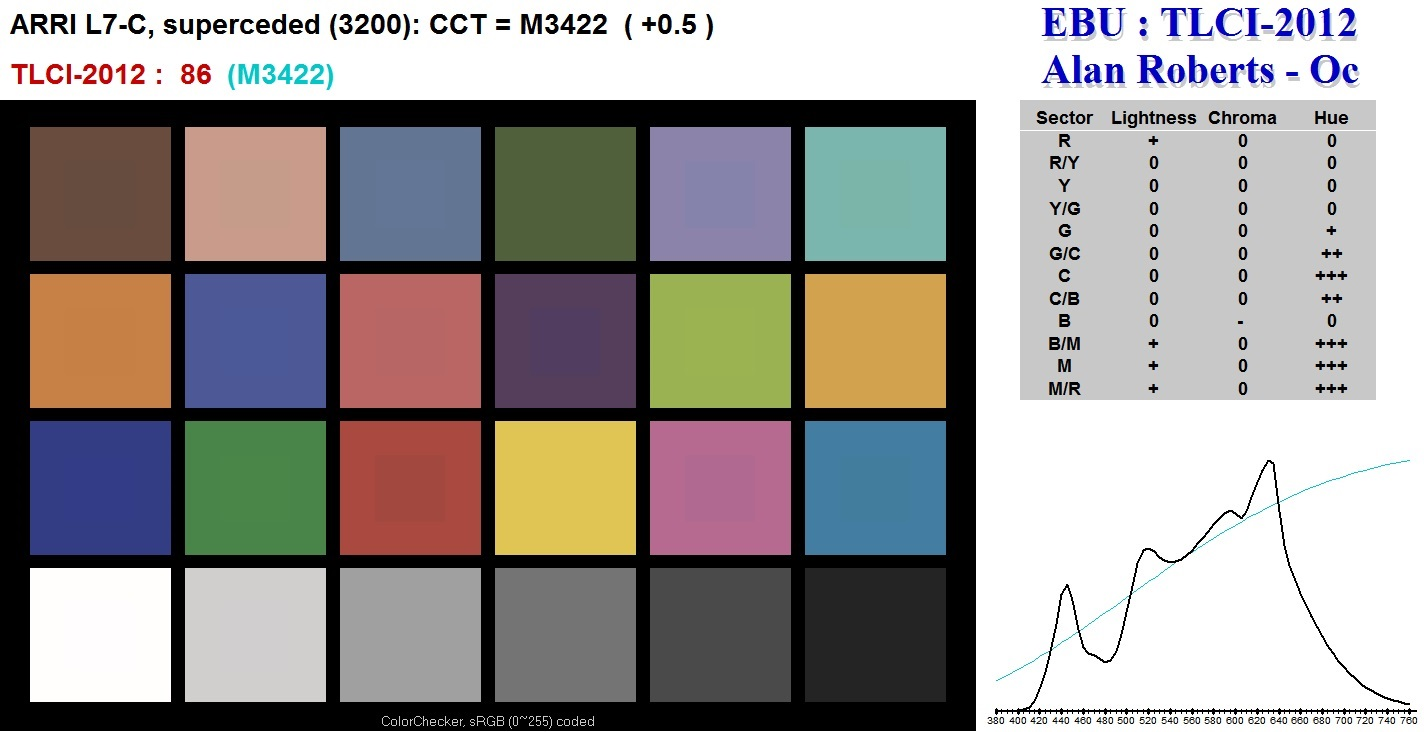
\includegraphics[width=1.0\textwidth]{bilder/tlci2} 
% Bilddatei aus dem Unterverzeichnis bilder holen, skalieren auf 0.8*Satzspiegel
\caption {TLCI-Ergebnisprotokoll eines Arri L7-C LED Fresnelscheinwerfers\protect\footnotemark}\label{b_tlci2}
\end{figure}
\footnotetext{\url{https://tech.ebu.ch/tlci-2012}}
\noindent Der Abbildung 4.7 kann links oben der Name der Leuchte, die gemessene korrelierte Farbtemperatur und die Abweichung vom Plank'schen Kurvenzug (Kapitel\ref{sec_farbtemperatur}) mit einer Gewichtung von 0.0054 (Empfehlung EBU) entnommen werden. Ist der Abweichungswert kleiner als -1 wird die Zahl in magenta dargestellt (magentastichtiges weiß), ist sie größer als +1, in grün (grünstichiges weiß). Da die Leuchte keine farbliche Abweichung aufweist, ist die in der Abbildung zu sehende Zahl schwarz. Eine Zeile darunter steht der gemessene TLCI-Wert. Der Arri L7-C ist mit $Q_{a}=86$ in die beste Farbwiedergabekategorie einzuordnen (Tabelle \ref{t_tlci}).\\
Die Tabelle rechts oben zeigt Korrekturvorschläge für eine weitere Bildbearbeitung. In diesem Beispiel wurden für 12 Farbtöne Verbesserungen für die Helligkeit, die Sättigung und/oder die Farbtonabweichung ermittelt. Da es nicht möglich ist, die Abweichung der Werte mit exakten Zahlen zu definieren, werden mit \glqq +\grqq\ , \glqq 0\grqq\ und \glqq -\grqq\ die verschiedenen Korrekturrichtungen aufgezeigt. Eine \glqq 0\grqq\ zeigt an, dass der Fehler so minimal ist, dass eine Korrektur nicht notwendig ist. Die Anzahl der \glqq +\grqq\ und \glqq -\grqq\ wiederum ist ein Hinweis darauf, wie viel Aufwand der Colorist für die Anpassung benötigt. Bei dem in diesem Beispiel vermessenen Arri L7-C Bedarf es vorallem im Bereich der Farbtöne Cyan, Blau/Magenta, Magenta und Magenta/Rot einer Aufbesserung. Auch im Grün/Cyan- und Cyan/Blau-Bereich sollte der Farbton angepasst werden. Die empfohlenen Verbesserungen der Helligkeit und Sättigung einiger Farbtöne sind nach der Tabelle bzw. dem gemessenen Ergebnis weniger umfangreich.\\
Eine Farbtafel mit 24 farbigen Rechtecken ist in der Abbildung 4.7 unten links sichtbar. Dabei beinhaltet jedes rechteckige Farbfeld mittig ein weiteres, kleines Rechteck, welches die Referenzfarbe anzeigt. Das große, äußere Farbfeld zeigt dabei die Farbe, die in diesem Fall der Arri L7-C wiedergibt. Je deutlicher das Referenzviereck in dem Farbfeld zu sehen ist, desto schlechter ist die Farbwiedergabe der Testleuchte. Im gezeigten Beispiel ist vor allem im roten Farbfeld ein deutlicher Unterschied zu erkennen aus dem sich schließen lässt, dass der Arri L7-C diese Farbe weniger gut wiedergibt wie andere Farben.\\ 
Rechts unten ist auf dem TLCI-Ergebnisprotokoll das Referenzspektrum mit dem Wellenlängenbereich von 380 nm bis 740 nm abgebildet (schwarz) und dazu wird das geteste Spektrum geplottet (cyan). In dieser Ansicht kann man gut erkennen, inwieweit das Licht des Arri L7-C das Referenzspektrum abdeckt\footnote{\cite[15]{roberts}}.\\

Zusammenfassend lässt sich sagen, dass der TLCI die Farben für eine Kamera bewewertet und zieht sogar zwei Hauttöne mit in Betracht. Daher eignet sich dieser Farbwiedergabewert sehr gut für die Messung der Auswirkung eines Red Tail.  



\section{IES Method for Evaluating Light Source Color Rendition (TM-30-15)} \label{sec_tm30}

Der TM-30 wurde 2015 von der \glqq Illuminating Engineering Society\grqq\ (IES) ausgearbeitet um eine Alternative zum CRI zu finden. Wie beim CRI werden ebenso bei der Messung des TM-30 Farbunterschiede zwischen einer Testleuchte und Referenzwerten der selben korrelierten Farbtemperatur aufgezeigt. Der TM-30 differenziert ähnlich, ob es sich bei der Testleuchte um einen Plank'schen Strahler oder einen Tageslichtscheinwerfer handelt. Zwischen einer CCT von 4500 K und 5500 K wird die Referenz proportional überblendet, um so zu verhindern, dass es bei 5000 K einen \glqq Sprung\grqq\ gibt. Bei dem CRI konnte es nämlich passieren, dass eine Leuchte 2 unterschiedliche Referenzen bekam, je nach dem ob diese knapp über oder unter 5000 K bei der Messung lag. 
Die 99 Referenzfarben (Color Evaluation Sample) wurden aus einem Pool von 105.000 Farbtönen realer Objekte statistisch ermittelt (Abbildung \ref{b_tm301}). Damit alle Farbtöne gleichmäßig abgedeckt werden, wurde der CAM02-UCS-Farbraum, der für seine Gleichmäßigkeit der Farbaufteilung bekannt ist, in Würfel eingeteilt. Von jedem dieser Würfel wurde dann eine der Referenzfarben bestimmt, die so gewählt ist, dass die unterschiedliche Wahrnehmung der verschiedener Wellenlänge minimal ist (Kapitel \ref{sec_auge}). Die große Anzahl der Referenzfarben verhindert, dass Leuchtenhersteller mit gezielten Peaks im Spektrum gute TM-30 Werte erreichen \footnote{\cite{usdep}}.
\newpage

\begin{figure}[H]     % h=here, t=top, b=bottom, p=page
\centering
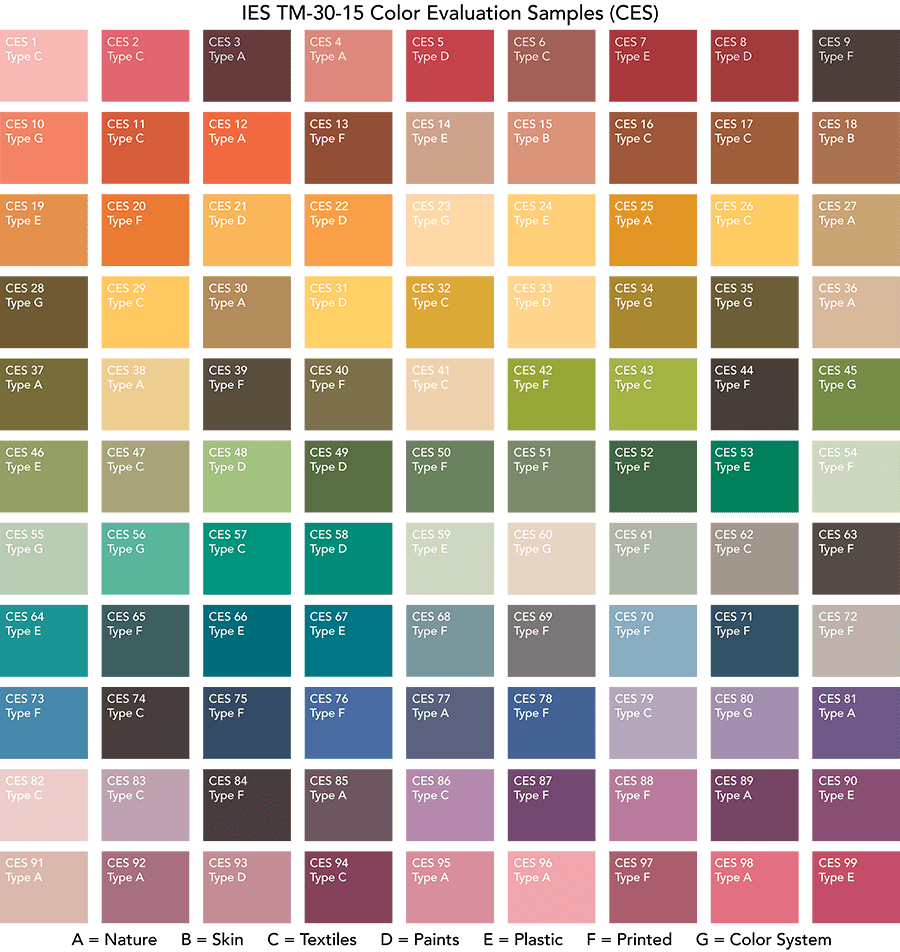
\includegraphics[width=1.0\textwidth]{bilder/tm301} 
% Bilddatei aus dem Unterverzeichnis bilder holen, skalieren auf 0.8*Satzspiegel
\caption {Alle 99 Referenzfarben des TM-30\protect\footnotemark}\label{b_tm301}
\end{figure}
\footnotetext{\url{https://agustos.com/wp-content/uploads/2017/10/TM30-color-samples-image.png}}


Im Gegensatz zum CRI spielen beim TM-30 zwei Werte eine große Rolle: $R_{f}$ und $R_{g}$. Der $R_{f}$-Wert bildet analog zum $R_{a}$-Wert des CRI ein Mittel aus den neunundneunzig Farbunterschieden denen einen Wert von 0 - 100 zugeordnet wird. Auch der $R_{f}$-Wert zeigt nicht an, ob die Leuchte übersättigte Farben hat oder einen Farbshift(\footnote{\cite[10]{royerhouser}}). Dazu wird der $R_{g}$-Wert gemessen. Dieser kann zwischen 60 und 140 variieren und zeigt so, ob die Farben übersättigt ($R_{g} > 100$), untersättigt ($R_{g} < 100$) sind oder mit dem Wert $R_{g} = 100$ genau die Farben der Referenzleuchte (bei selbiger Farbtemperatur) treffen. Mit dem $R_{f}$- und $R_{g}$-Wert wird ein X,Y-Koordinatensystem aufgespannt (Abbildung \ref{b_tm302}). Aus diesem Diagramm sind Farbwiedergabeeigenschaften einer Leuchte sehr gut ablesbar. Durch den zusätzlichen $R_{g}$-Wert gibt es nicht mehr nur Leuchten mit \glqq guter\grqq\ (hoher (hoher $R_{f}$)) oder \glqq schlechter\grqq\ (niedriger $R_{f}$) Farbwiedergabe. Zum Beispiel verliert eine Leuchte mit $R_{f}=82$ und $R_{g}=127$ gegenüber einer mit $R_{f}=90$ und $R_{g}=98$ nicht unweigerlich. Es kommt im direkten Vergleich viel mehr auf den Anwendungsfall an, in der die Leuchte gebraucht wird. Im sterilen Krankenhaus ist eine natürlich Farbwiedergabe wichtig, dort wäre die zweite Leuchte der Favorit, wohingegen für Superläden, in denen das Obst durch Übersättigung der Farben besser zur Geltung kommt, wäre die erste Lampe attraktiver. 
Daher ist der TM-30 viel flexibler zu deuten als der CRI, wo es immer nur um den höchsten $R_{a}$-Wert geht. Eine Möglichkeit könnte es sein, das X,Y-Koordinatensystem in verschiedene Bereiche(z.B. Fenster) einzuteilen, um so anwendungsspezifische Entscheidungen treffen zu können (\footnote{\cite[4]{royer}}).  


\begin{figure}[H]     % h=here, t=top, b=bottom, p=page
\centering
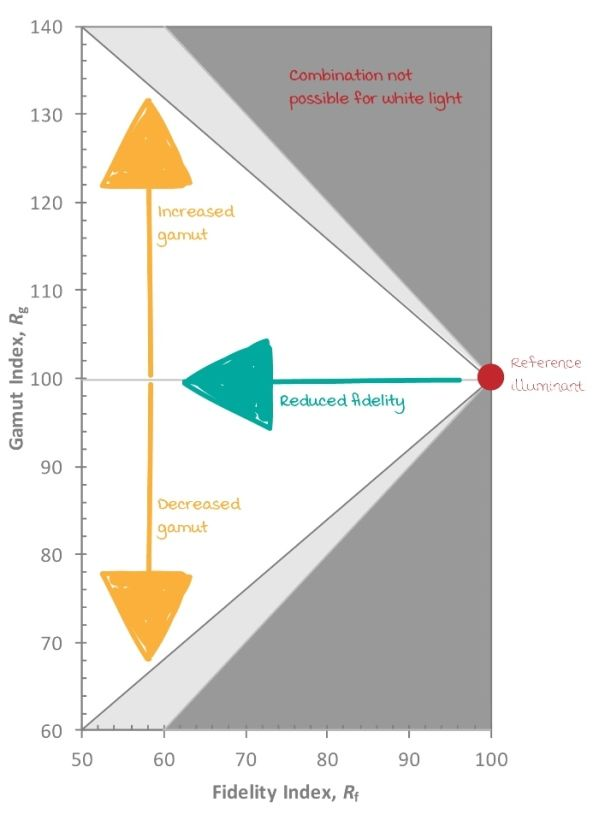
\includegraphics[width=0.5\textwidth]{bilder/tm302} 
% Bilddatei aus dem Unterverzeichnis bilder holen, skalieren auf 0.8*Satzspiegel
\caption {Koordinatensystem aus $R_{f}$ und $R_{g}$: Die hellgraue Zone steht für TM-30-Werte die nicht auf der Plank'schen Kurve liegen und die dunkelgraue Zone steht für alle Werte, die nicht mehr als \glqq weiß\grqq\ angesehen werden. \protect\footnotemark}\label{b_tm302}
\end{figure}
\footnotetext{\url{https://i.pinimg.com/originals/18/98/de/1898de3bdd8436fb5a1945d72a4c6772.jpg}}

In einer anderen Darstellung des $R_{g}$-Wert ist zu sehen, dass der Farbraum in 16 verschiedene \glqq binnings\grqq\ eingeteilt wurde. Jedes dieser \glqq binnings\grqq\ steht übergreifend für die in diesem Bereich liegende Farbtöne. In dieser Darstellung wird mit Pfeilen aufgezeigt, welche Anteile im Farbraum fehlen, welche übersättigt sind und welche den Farbton nicht treffen im Verhältnis zur Referenzfarbwiedergabe (Abbildung \ref{b_tm303}).

\begin{figure}[htp]     % h=here, t=top, b=bottom, p=page
\centering
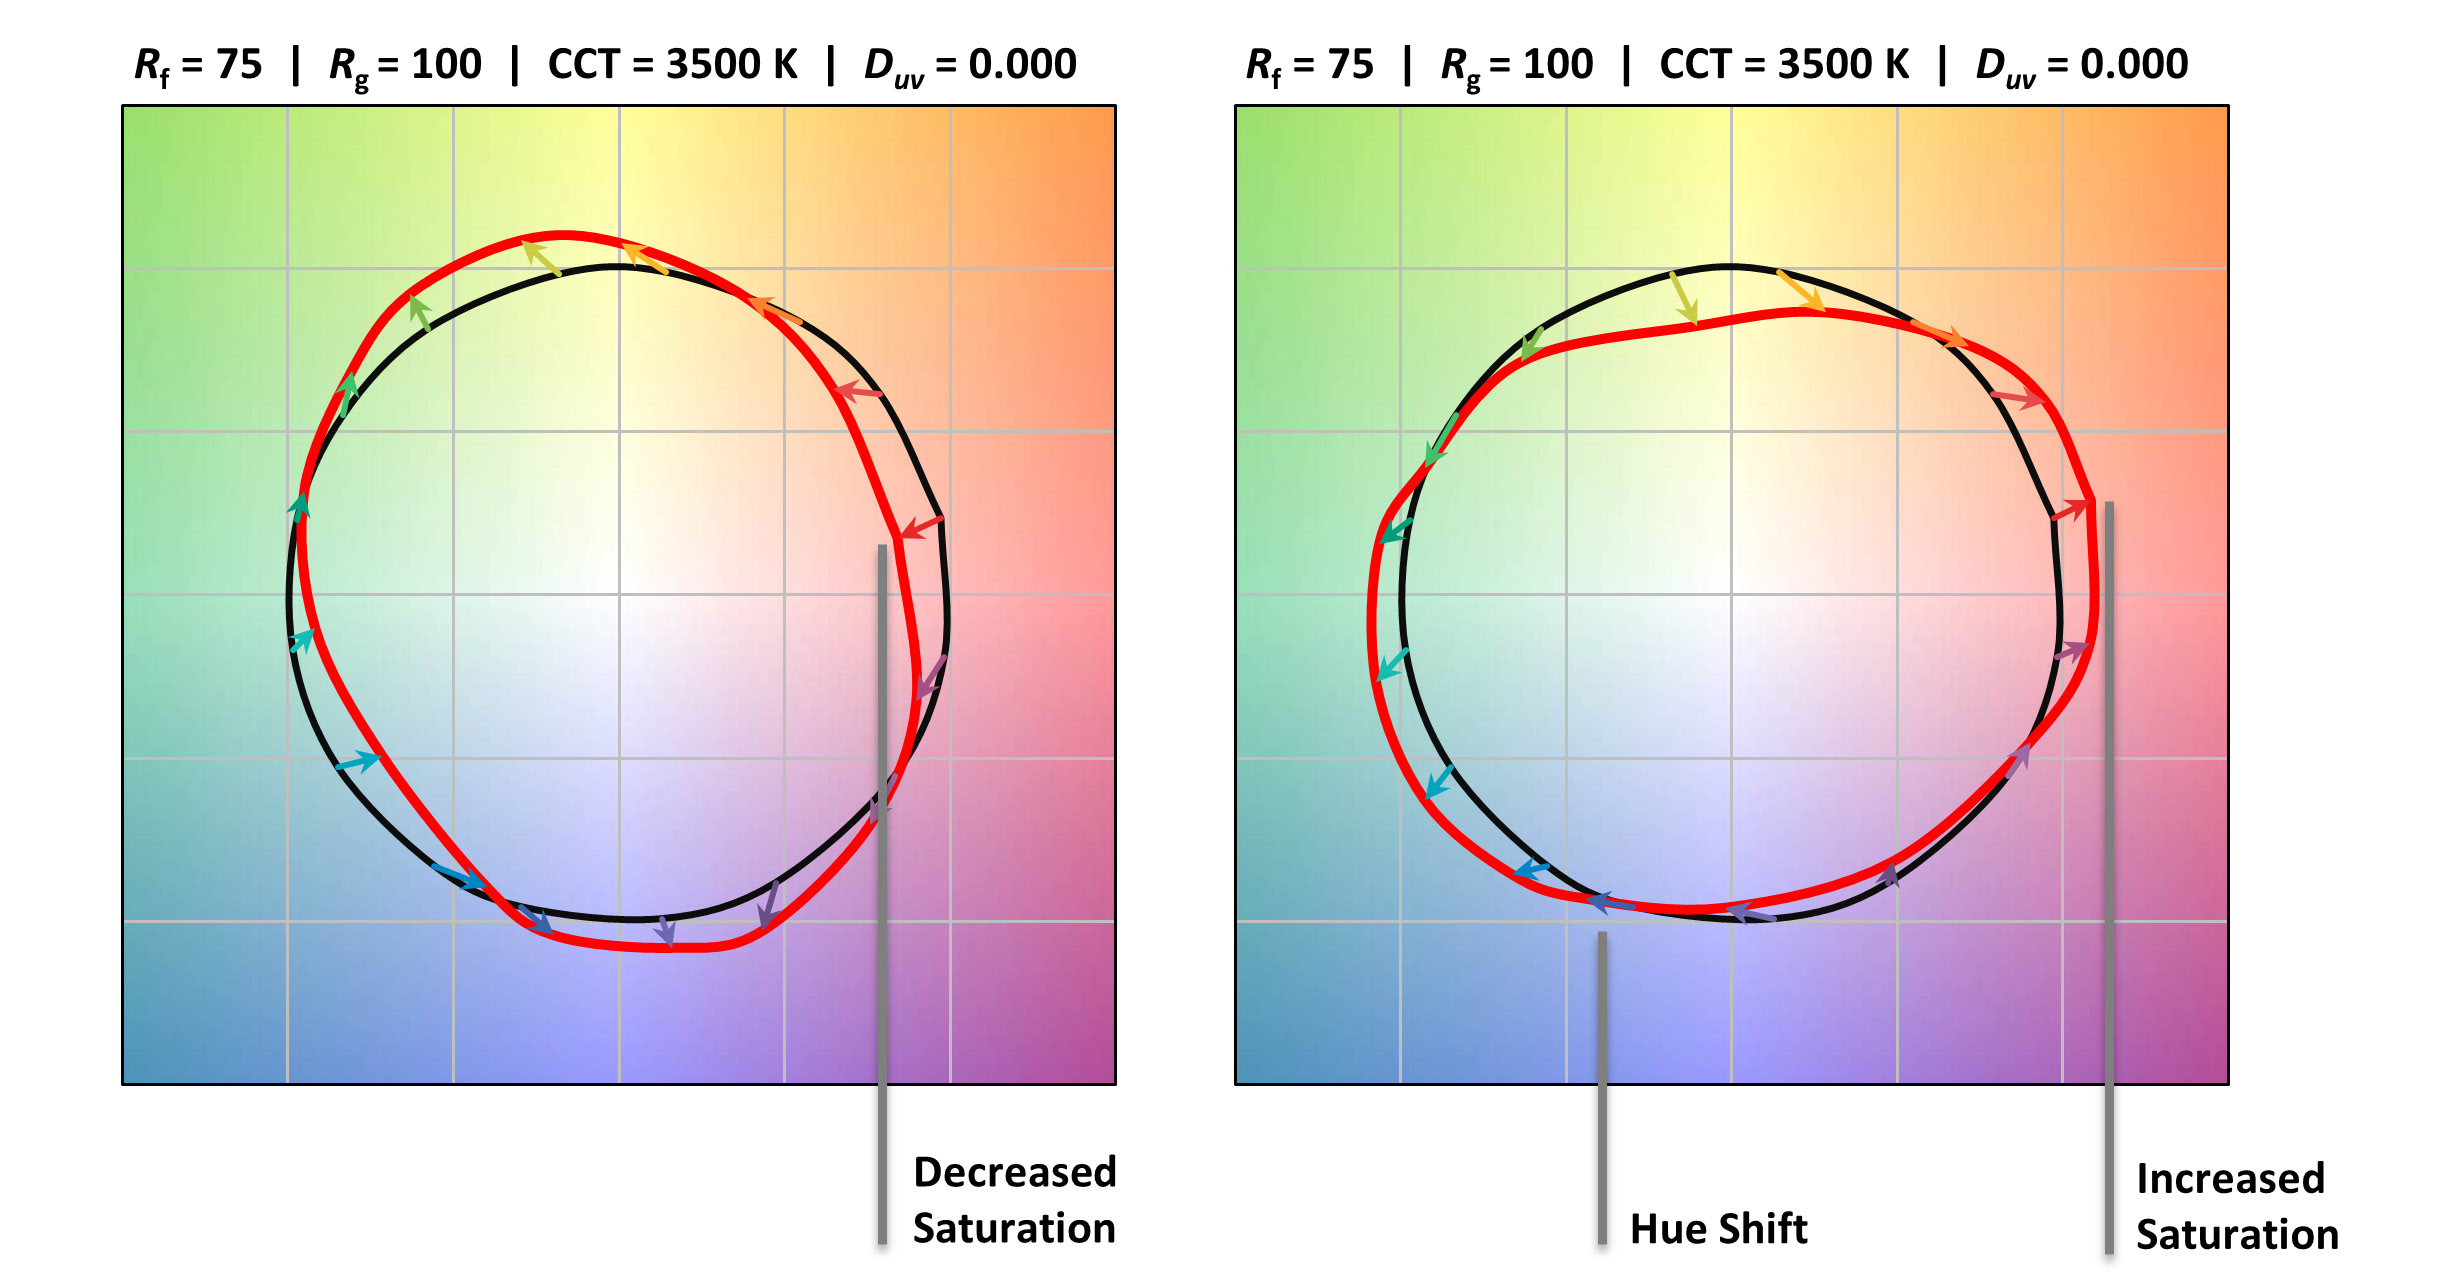
\includegraphics[width=1.0\textwidth]{bilder/tm303} 
% Bilddatei aus dem Unterverzeichnis bilder holen, skalieren auf 0.8*Satzspiegel
\caption {Wie sich die Farben der Testleuchte verhalten ist in der Vektorgraphik des $R_{g}$-Wertes anschaulich dargestellt. Der schwarze Kreis stellt die Referenzleuchte dar, der rote die getestete.  \protect\footnotemark}\label{b_tm303}
\end{figure}
\footnotetext{\cite{usdep}}

Bei der Messung einer Demo warmweiß LED gibt es viel an Messergebnissen zu protokollieren (Abbildung \ref{b_tm304}): Links oben wird gemessene $R_{f}$- und $R_{g}$-Wert angezeigt. Darunter ist die Vektorgraphik des $R_{g}$-Wertes dargestellt und darunter werden die $R_{f}$-Werte der 16 Farbraum-\glqq binnings\grqq\  in einem Säulendiagramm präsentiert. In der Mitte ist der TM-30-Wert in seiner Koordinaten Darstellung aufzufinden und darunter werden die farblichen Abweichungen (in Prozenten) in einem Säulendiagramm dargestellt. Rechts oben wird analog zum TLCI das Spektrum der Leuchte im Verhältnis zum Referenzspektrum gezeigt und die gemessene korrelierte Farbtemperatur angegeben. Darunter gibt es eine Tabelle wo die farblichen Abweichung der einzelnen \glqq binnings\grqq\ als Zahlenwert angegeben werden. Schließlich findet man unter allem bisher genannten eine Säulendiagramm mit allen 99 Farben des TM-30. 
Das Ergebnis einer Messung ist mit diesen Daten nicht mehr schnell ersichtlich, wie beim CRI-Wert, hilft aber eine deutlich aussagekräftigere Entscheidung über eine Leuchte treffen zu können. 

\begin{figure}[H]     % h=here, t=top, b=bottom, p=page
\centering
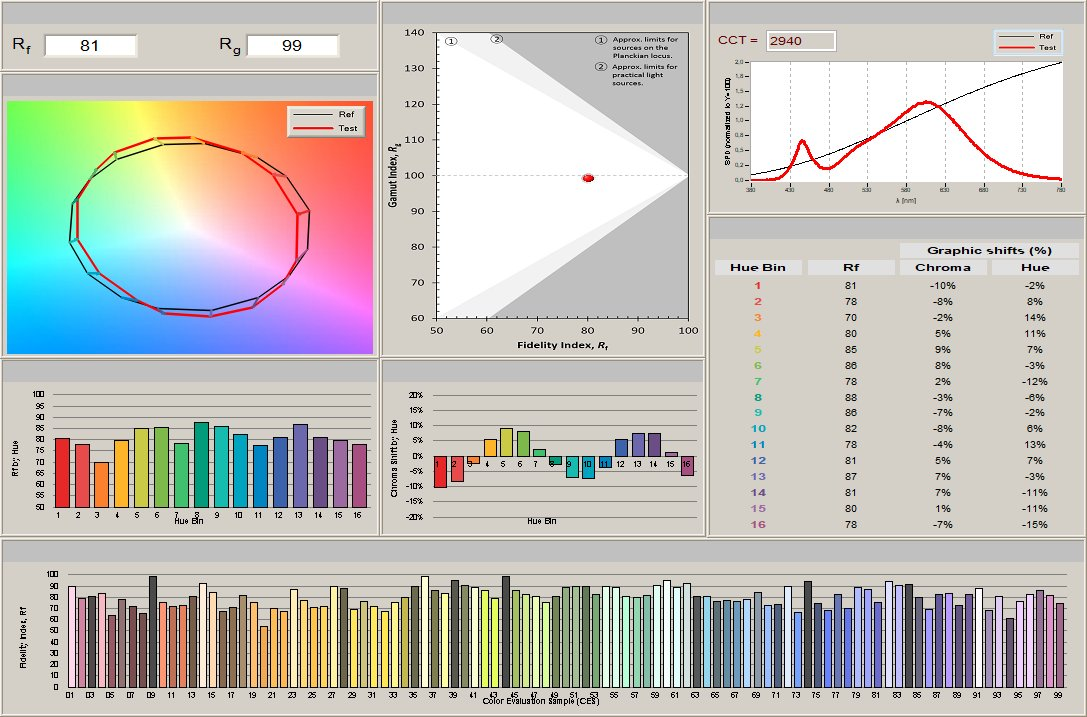
\includegraphics[width=1.0\textwidth]{bilder/tm304} 
% Bilddatei aus dem Unterverzeichnis bilder holen, skalieren auf 0.8*Satzspiegel
\caption {Wie sich die Farben der Testleuchte verhalten ist in der Vektorgraphik des $R_{g}$-Wertes anschaulich dargestellt. Der schwarze Kreis stellt die Referenzleuchte dar, der rote die getestete.\protect\footnotemark}\label{b_tm304}
\end{figure}
\footnotetext{\cite{usdep}}

Der TM-30 
%fertig schreiben

\chapter{Messgeräte für Farbmessung}
Es gibt die verschiedensten lichttechnischen Messgeräte, die genutzt werden um Beleuchtungsstärke, Farbtemperatur oder Farbigkeit des Lichts zu messen. Da in der Hauptmessung fast ausschließlich LED-Scheinwerfer gemessen werden, ist es wichtig, dass die Messgeräte in der Lage sind, mit diesem zum Teil schmalbandigen Spektren umzugehen. Dazu eignen sich am besten Spektrometer, die durch ihre sehr filigrane Messweise einzelner Wellenlänge auch extremere Spektren auswerten können. Zusätzlich können sie aus dem gemessene Spektrum viele lichttechnische Daten errechnen und sind damit die \glqq Alleskönner\grqq\ unter den Messgeräten. In diesem Kapitel soll ihre Funktionsweise erörtert werden.
 
\section{Spektrometer}
Ein Spektrometer besteht üblicherweise aus einem Eingangsspalt, einem Streuelement (Prisma oder Gitter) und aus einem einzeln Detektor oder aus einem Detektor-Array. Die für die Messungen verwendeten Spektrometer JETI specbos 1211 (Abbildungen \ref{b_jeti})und UPRtek MK350S (Abbildungen \ref{b_mk350s}) nutzen beide ein flat-field-Gitter mit einem Detektor-Array.

\begin{figure}
\begin{minipage}[hbt]{0.49\textwidth}
	\centering
	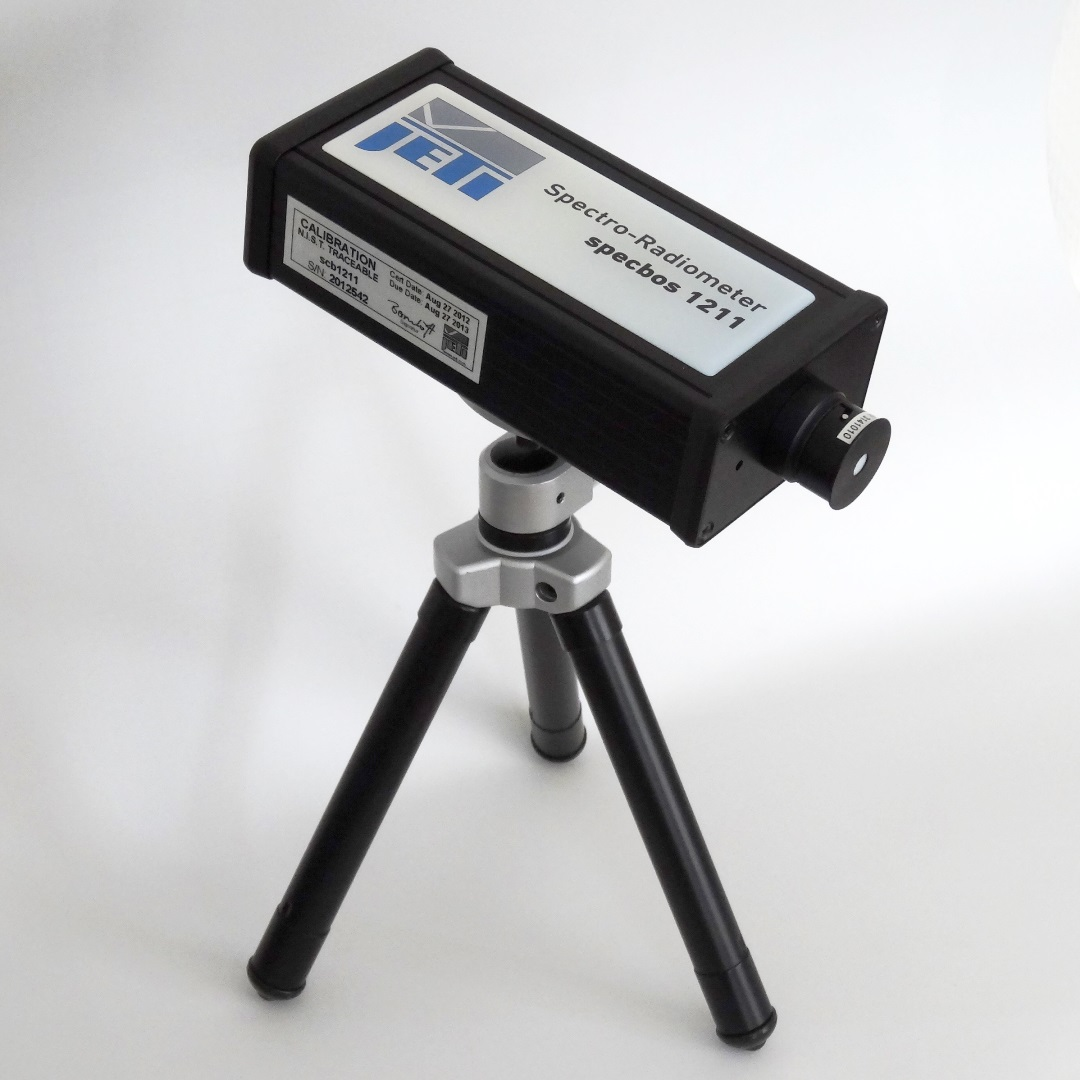
\includegraphics[width=0.49\textwidth]{bilder/jeti}
	\label{b_jeti}
	\setcounter{mpfootnote}{\value{footnote}}
      \renewcommand{\thempfootnote}{\arabic{mpfootnote}}
       \caption{Hauptmessgerät}
      Jeti Specbos 1211\footnote{\url{https://www.opteema.com/media/specbos4000.jpg}}
        \setcounter{footnote}{\value{mpfootnote}}
\end{minipage}
\hfill
\begin{minipage}[hbt]{0.49\textwidth}
	\centering
	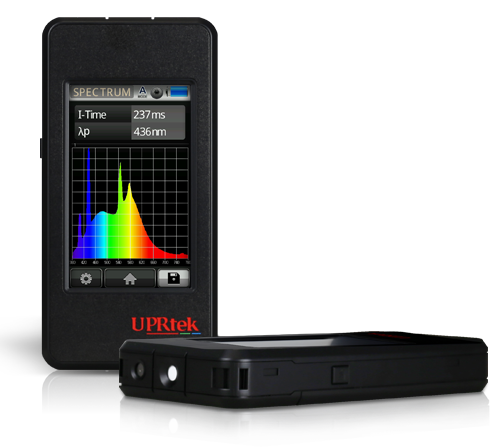
\includegraphics[width=0.49\textwidth]{bilder/mk350s}
	\label{b_mk350s}
	\setcounter{mpfootnote}{\value{footnote}}
      \renewcommand{\thempfootnote}{\arabic{mpfootnote}}
      \caption{Sekundärmessgerät}
      UPRtek MK350S\footnote{\url{https://www.opteema.com/media/specbos4000.jpg}}
            \setcounter{footnote}{\value{mpfootnote}}
\end{minipage}
\end{figure}





Das im Messgerät ankommende Licht gelangt durch den Spalt  ins Messgerät und wird auf das Reflexionsgitter geleitet. Dort interferiert das Licht und wird in seine einzelnen Wellenlängen aufgesplittet (Gleichung \ref{gl_spek1}).
\begin{equation}\label{gl_spek1}
		sin(\Theta_{M})=sin(\Theta_{i})+m \frac{\lambda}{d}
\end{equation}
$\Theta$ beschreibt jeweils den Ein- und Austrittswinkel des Lichts. $\lambda$ steht für die Wellenlänge des Lichts, d für die Gitterkonstante und m für die Ordnungszahl der Interferenz. Durch die optischen Eigenschaften eines Reflexionsgitters werden die verschiedenen Wellenlängen in unterschiedlichen Winkeln aufgesplittet und so ist es möglich, dass das Spektrometer ein Spektrum sehr fein auflösen kann (Abbildung \ref{b_spek1}). Es wird nur das reflektierte Licht einer bestimmten Ordnungszahl m ($m \neq 0$) bei einer Messung genutzt. Die zusätzlich entstandenen Reflexionen andere Ordungszahlen sind zu ignorieren\footnote{\cite[6]{jeti}}. 

\begin{figure}[htp]     % h=here, t=top, b=bottom, p=page
\centering
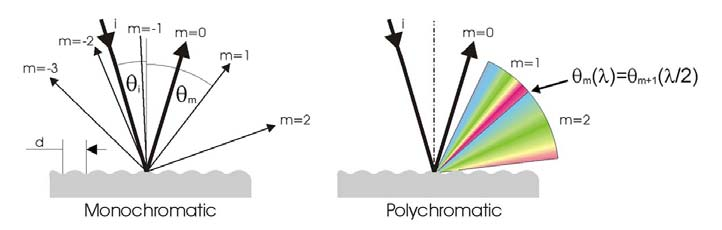
\includegraphics[width=1.0\textwidth]{bilder/spek1} 
% Bilddatei aus dem Unterverzeichnis bilder holen, skalieren auf 0.8*Satzspiegel
\caption {Abbildung der Interferenz am optischen Gitter\protect\footnotemark}\label{b_spek1}
\end{figure}
\footnotetext{\cite[6]{jeti}}

Bei einem flat-field-Gitter liegt der Vorteil, dass das interfierte Licht schon gebündelt wird, da dieses Gitter konkav gebaut ist und damit als ein Hohlspiegel dient\footnote{\cite{wiki}}. So werden weniger optische Elemente gebraucht und kosten gespart \footnote{\cite[7]{jeti}}.\\
Nachdem das Licht durch das optische Gitter reflektiert wurde, trifft es auf das Detektor-Array. Es werden normalerweise CCD-Sonsoren, oder CMOS-Sensoren als Detektor-Array genutzt:

\begin{itemize}
\item CCD-Sensor (charge-coupled device): Dieser Sensor ist aus einer Anordnung von lichtempfindlichen Fotodioden, die auf einem Halbleiter aufgebaut sind. Die Fotodioden sind mit einer Spannung versorgt. Trifft nun das Licht auf die Fotodioden lösen sich Elektronen, die in Potentialtöpfen gesammelt werden. Diese Potentiale werden in den Speicherbereich verschoben, damit wieder neues Licht die Fotodioden anregen kann. Der Sensor wird ausgelesen, indem die Potentiale sequentiell in den Ausgabebereich verschoben und dort in Spannungen umgewandelt werden. Dabei werden nur die Spannungsunterschiede zwischen den davor ausgelesen Werten verwendet, damit das Rauschen des Sensors gering gehalten wird. Für den ersten Spannungsunterschied wird ein Referenzwert festgelegt\footnote{\cite[17]{jeti}}.

\item CMOS-Sensor (complementary metal-oxide-semiconductor): Dieser Sensor ist aus Fotodioden aufgebaut, die jeweils in Sperrichtung mit zum Beispiel drei Transistoren betrieben werden. Wenn Licht auf die Fotodioden trifft wird die Sperrschichtkapazität durch den Photostrom entladen und der Spannungswert wird direkt auf dem Pixel ausgelesen\footnote{\cite[369]{schmidt}}.

\end{itemize}
Es können auch nur eine Ansammlung von Fotodioden im Zusammenspiel mit einem analogen switch als Detektor-Array genutzt werden\footnote{\cite[18]{jeti}}. Dies hat jedoch für diese Abeit keine relevanz, da nur Messgeräte mit CMOS- bzw. CCD-Sensor genutzt werden.\\

Das Licht wird bei Spektrometern gemäß den Farbfunktionen $\phi(\lambda)$ des Auges gemessen (Kapitel \ref{sec_colour}). Diese werden dann in die X,Y und Z Primärvalenzen des CIE-XYZ Farbraums umgerechnet (Kapitel \ref{sec_xyz}). Im XYZ-Farbraum werden schließlich die Farbkoordinaten des gemessenen Lichts bestimmt\footnote{\cite[30]{jeti}}. Auch die Farbwiedergabewerte errechnen wird aus dem gemessenen Spektrum berechnet(Kapitel \ref{sec_cri}).\\

Der JETI specbos 1211 wird in den Hauptmessung als Primärmessgerät genutzt und mit dem UPRtek 350S sollen diese Werte zur Messsicherheit überprüft werden. Folgende Tabelle soll einige Unterschiede der Messgeräte aufzeigen:

\begin{table}[htp] 
		\rowcolors{1}{}{lgray} 
		\centering
		\begin{tabular}{rlcc}  % Spalten nach Ausrichtung: l, c, r, p{breite} 
		\toprule
		\multicolumn{3}{c}{\large\sffamily Spektrometervergleich}\\ 							
		\midrule
		Spektrometer & JETI specbos 1211 & UPRtek 350S\\
		Variante & PC gebunden & handheld\\
		Sensor & CCD array 2048 pixel & CMOS Linear Image Sensor\\
		Streuelement & flat-field-Gitter & flat-field-Gitter\\
		Spektraler Messbreich & 350 nm - 1000 nm & 380 nm - 780 nm\\
		Beleuchtungsstärke & 2 lux - 60.000 lux & 1 lux - 100.000 lux\\
		Farbgenauigkeit &  $\pm 0,002$ x,y & $\pm 0,0025$ x,y\\
		Farbwiedergabe &  $\pm 0,0005$ x,y & $\pm 0,0005$ x,y\\		
		Farbtemperatur &  $\pm 2$ $\%$ & $\pm 20$ K\\
		\bottomrule
		\end{tabular}
		\caption{Vergleich zweier Spektrometer\protect\footnotemark}	
		\label{t_spek}
	\end{table}
\footnotetext{\cite{jetii} \cite{uprtek}}

Der JETI specbos 1211 hat eine genauerer Farbeinschätzung des Lichtes und eine geringere Abweichung bei der Farbtemperatur (Tabelle \ref{t_spek}). Alle Messwerte beziehen sich auf eine Messung der CIE-Normlichtart A mit 2.856 K, damit Messgeräte vergleichbar sind.




\chapter{Grundlagen Videotechnik}
Da sich diese Arbeit auch mit der Lichtwirkung im Zusammenhang mit Kameras beschäftigt, sollen in diesem Kapitel die relevanten videotechnischen Grundlagen dargestellt werden.

\section{Grundeinstellung einer Kamera}

\subsection{Vorverstärkung}
\label{sec_gain}
Mit der \glqq Gain up\grqq -Funktion einer Kamera kann die Helligkeit des Bildes elektrisch nachreguliert werden. Falls die Bleuchtungsstärke beispielsweise zu gering ist , kann so über einen Regler in verschiedenen Stufen (meist in 1 dB oder 3 dB Schritten) das Bild vorverstärkt werden. Die Einheit Dezibel (dB) ist logarithmisch. Bei einer Verstärkung von +6 dB ist das Bild doppelt so hell. Durch eine elektrische Beeinflussung des Bildes erhöht sich jedoch auch stets das Bildrauschen im selben maße. Eine Verstärkung von +3 dB erhöht ebenso das Bildrauschen um +3 dB. Daher sollte man das Videosignal nicht zu stark elektrisch vorverstärken\footnote{\cite[406-407]{schmidt}}.\\
Die Vorverstärkung wird während der Erstellung der Bilder in der Hauptmessung genutzt, um Helligkeiten der Scheinwerfer, an die Kamera anzugleichen.

\subsection{Blende}
\label{sec_blende}
Die Blende ist die mechanische Öffnung im Objektiv, mit dem die Lichtmenge, die auf den Bildwandler (Kapitel \ref{sec_wandler}) trifft, reguliert werden kann. Sie wird über den Blendenring an der Kamera eingestellt. Je höher die Blende gewählt wird, desto weniger Licht lässt die mechanische Öffnung passieren. Typische Zahlenangaben für eine Blende ist die Blendenreihe, in der die Zahlen immer in Abhängigkeit von $\sqrt{2}$ ansteigen: \\
f/1,4  f/2  f/2,8  f/4  f/5,6  f/8  f/11  f/16
Dabei werden die Blendenzahlen immer reziprok zur Brennweite f angegeben\footnote{\cite[387]{schmidt}}. Die Brennweite ist die Entfernung zwischen der Linse zu ihrem Brennpunkt\footnote{\cite{rosko}}. Je größer die Blende der Kamera eingestellt ist, desto mehr Licht wird benötigt, um durch die kleiner werdende Öffnung genug Helligkeit für den Bildwandler zubekommen (Abbildung \ref{b_blende}). Pro Blendenstufe halbiert bzw. verdoppelt man die Beleuchtungsstärke\footnote{\cite[388]{schmidt}}.\\
Die Kamera, die in der Hauptmessung genutzt wird ist eine Kamera die bei der Blende f/11 eine Beleuchtungsstärke von 2000 lux nutzt, damit das Bild ohne Vorverstärkung das volle Videosignal nutzt (Kapitel \ref{sec_wahlderKamera}). Das bedeutet, dass, wenn bei der Hauptmessung alle Scheinwerfer auf 500 lux Beleuchtungsstärke angepasst werden, diese Kamera nach der Blendenreihe mit einer Blende f/4 arbeitet. Die Blende wird bei der Hauptmessung tatsächlich auf f/3,7 eingestellt, damit eine halbe Blende Spielraum bleibt, die Helligkeit des Bildes über die Vorverstärkung zu beeinflussen (Kapitel \ref{sec_gain}). Das hat den Hintergrund, dass die Scheinwerfer beim Anpassen an die Kamera auch ihre Beleuchtungsstärke ändern. Um diese Veränderung wieder auszugleichen ist es praktikabler über die Vorverstärkung die Helligkeit anzupassen, als zu versuchen mit sehr kleinen Blendenzahlen den richtigen Wert zu treffen (Kapitel \ref{sec_anpassunglampen}).

\begin{figure}[htp]     % h=here, t=top, b=bottom, p=page
\centering
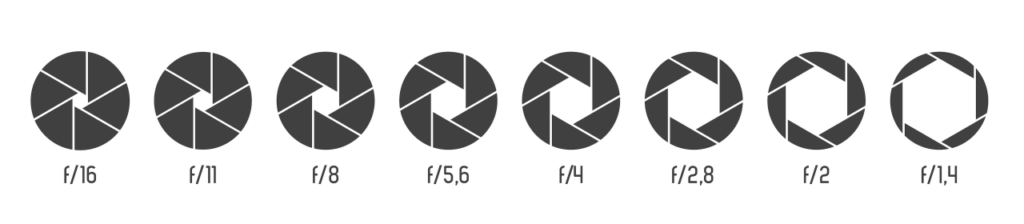
\includegraphics[width=1.0\textwidth]{bilder/blende} 
% Bilddatei aus dem Unterverzeichnis bilder holen, skalieren auf 0.8*Satzspiegel
\caption {Darstellung verschiedener Blendzahlen\protect\footnotemark}\label{b_blende}
\end{figure}
\footnotetext{\url{https://rogerhirt.ch/wp-content/uploads/2017/12/blende-1280x280-1024x224.png}}


\subsection{Schärfentiefe}
\label{sec_scharf}
Bei gleichbleibender Brennweite ist die Schärfentiefe des Bildes abhängig von der Blende. Diese Größe sagt aus, wie viele Anteile des Bildes im Hintergund und Vordergrund verschwimmen im Verhältnis zum scharfgestellten Bereich der Kamera. Eine kleine Blendenöffnung (zum Beispiel f/11) führt dazu, dass das Bild größenteils scharf dargestellt wird. Es gibt kaum Bildanteile die verschwimmen und somit wird von einer großen Schärfentiefe gesprochen. Umgekehrt führt eine offene Blende zu einem kleinen Teil der im Bild scharf dargestellt und einer geringen Schärfentiefe\footnote{\cite[389]{schmidt}} (Abbildung \ref{b_scharfentiefe}.\\
Da bei der Erstellung der Bilder nur Personen auf der selben Ebene dargestellt werden, liegt bei Blende 4 der Kamera die kleinere Schärfentiefe auf den fotografierten Probanden. Der Rest des Bildes erscheint unscharf.

\begin{figure}[htp]     % h=here, t=top, b=bottom, p=page
\centering
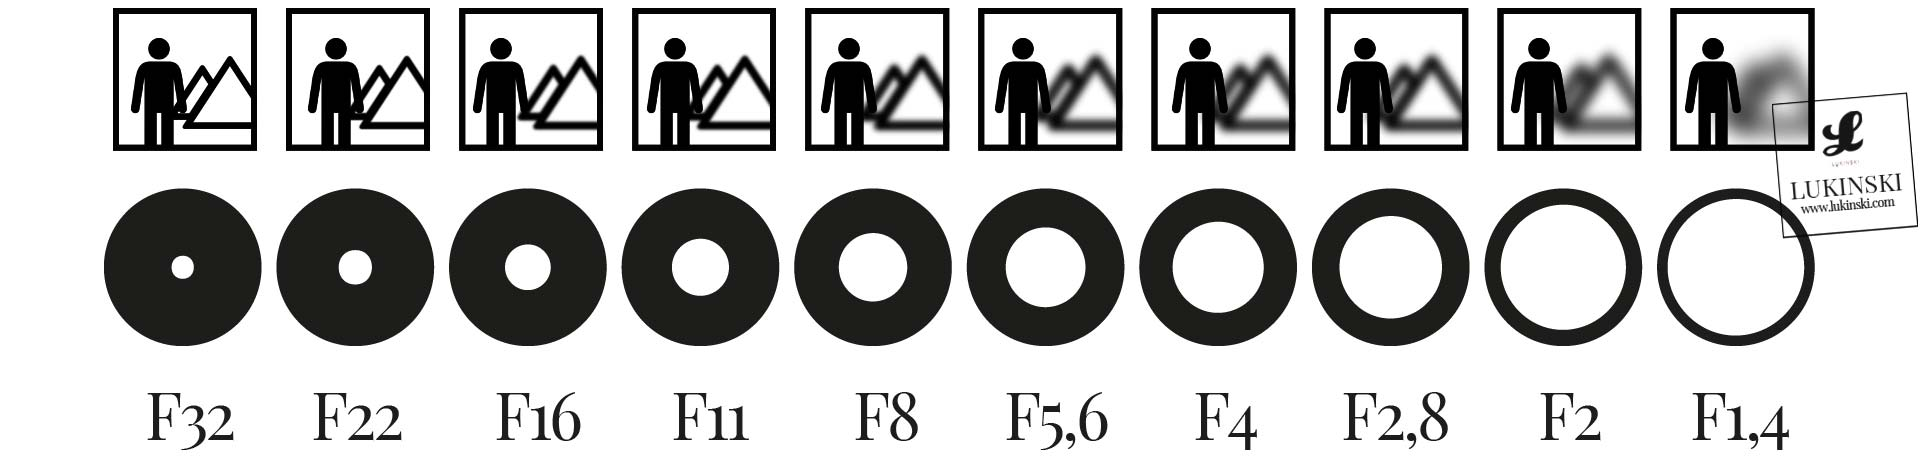
\includegraphics[width=1.0\textwidth]{bilder/scharfentiefe} 
% Bilddatei aus dem Unterverzeichnis bilder holen, skalieren auf 0.8*Satzspiegel
\caption {Darstellung der Schärfentiefe im Bezug zur Blende\protect\footnotemark}\label{b_scharfentiefe}
\end{figure}
\footnotetext{\url{https://www.google.com/url?sa=i&rct=j&q=&esrc=s&source=images&cd=&cad=rja&uact=8&ved=2ahUKEwiJo7D_k_fcAhWJZlAKHX4zAe4QjRx6BAgBEAU&url=https\%3A\%2F\%2Flukinski.de\%2Fblende-verschlusszeit-iso-wert-grundlagen-fotografie\%2F&psig=AOvVaw0Hqo1IBasaijczWBZx5BjU&ust=1534700237116015}}

\subsection{Kniefunktion}
\label{sec_knee}
Mit der Kniefunktion lässt sich verhindern, dass Bilder deren Helligkeit zu groß sind, Details in den übersteuerten Bereichen verlieren, da diese Pegelwerte (Kapitel \ref{sec_gamma}) normalerweise von der Kamera hart abgeschnitten werden. Durch das Aktivieren der Kniefunktion wird die Dynamik des Bildes erhöht und es können sogar Belichtung, die eine Blendenstufe zu hoch sind, im Bild zugelassen werden.\footnote{\cite[389]{schmidt}}.\\
Die Kniefunktion wird in der Kamera während der Erstellung der Bilder dazu genutzt, falls nach dem Angleichen der Scheinwerfer auf die Kamera, die Belichtung des Bildes zu hoch ist (Kapitel \ref{sec_anpassunglampen}).

\subsection{$\gamma$-Kennlinie}
\label{sec_gamma}
Die $\gamma$-Kennlinie beschreibt den Zusammenhang zwischen Lichtstrom und Videopegel. Der Videopegel beschreibt von 0 bis 100\% die Stärke des Videosignals. Diese $\gamma$-Kennlinie ist darauf zurückzuführen, dass die Fernseher mit Kathodenstrahlröhre die Videosignalpegel nur als verzerrte Leuchtdichtewerte ausgegeben haben. Die im Studio aufgenommenen Lichtverhältnisse kommen also nicht zu Hause beim Zuschauer an. Um diesem Umstand entgegen zu wirken, wird das Kamerasignal vorentzerrt (Abbildung \ref{b_gamma}). Aus diesen historischen Gründen ist die $\gamma$-Vorentzerrung des Videosignals geblieben. Ein Fernseher hat typischerweise einen $\gamma$-Wert von 2,2 und die Kamera folglich den Kehrwert von ca. $\gamma=0,45$.\footnote{\cite[408-409]{schmidt}}.\\
Alle Kamerasignale bei der Erstellung der Bilder für die Umfrage sind auch $\gamma$-vorentzert. Außerdem ist die TLCI-Messung mit einer Kamera auch mit $\gamma$ behaftet (Kapitel \ref{sec_tlci}).

\begin{figure}[htp]     % h=here, t=top, b=bottom, p=page
\centering
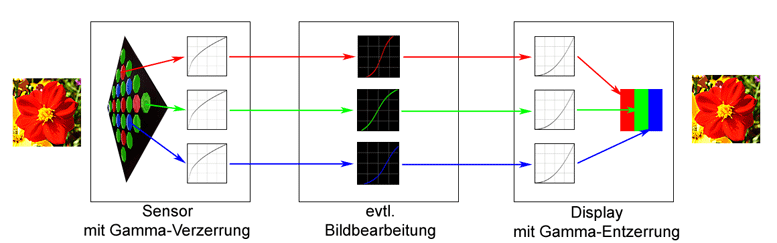
\includegraphics[width=1.0\textwidth]{bilder/gamma} 
% Bilddatei aus dem Unterverzeichnis bilder holen, skalieren auf 0.8*Satzspiegel
\caption {Darstellung der $\gamma$Vorentzerrung und Rückkorrektur\protect\footnotemark}\label{b_gamma}
\end{figure}
\footnotetext{\url{http://www.simpelfilter.de/farbmanagement/images/grafik_farbuebertragung.gif}}

\subsection{Linear Matrix}
\label{matrix}
Die Matrix einer Kamera ist für eine Korrektur der Farbwiedergabe nötig. Denn die Spektralwertkurven eines Bildwandlers können keine negativen Spektralanteile aufzeichnen können (Kapitel \ref{sec_wandler}). Die Bildschirme nutzen aber die Primärvalenzen der EBU, die wiederum mit negativen Werten arbeiten. Die lineare Matrix macht es nun möglich, dass die Spektralwertanteile von dem Bilderwandler auf die Bildschirmebene transformiert wird.\footnote{\cite[412-413]{schmidt}}.\\
Die Notwendigkeit der Transformation zeigt, dass die Kamera Spektren deutlich anders bewertet als das menschliche Auge und damit auch als lichttechnische Messgeräte (Abbildung \ref{b_matrix}) Das spielt eine große Rolle für das weitere Vorgehen bei der Erstellung der Bilder während der Hauptmessung (Kapitel \ref{sec_anpassunglampen}).

\begin{figure}[H]     % h=here, t=top, b=bottom, p=page
\centering
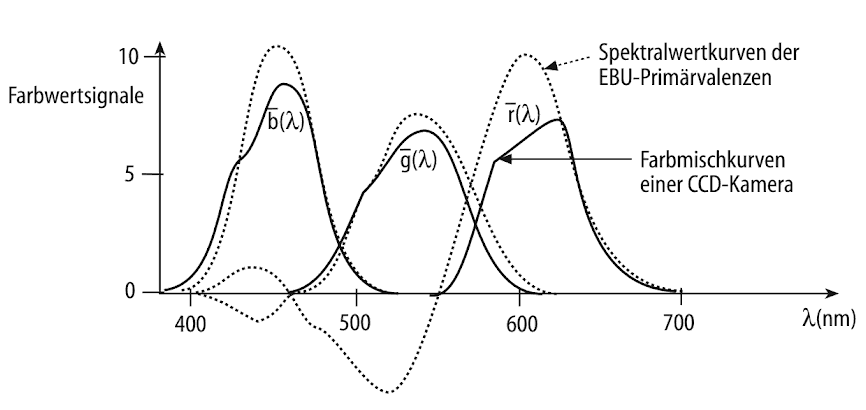
\includegraphics[width=1.0\textwidth]{bilder/matrix} 
% Bilddatei aus dem Unterverzeichnis bilder holen, skalieren auf 0.8*Satzspiegel
\caption {Darstellung der $\gamma$-Vorentzerrung und Rückkorrektur\protect\footnotemark}\label{b_matrix}
\end{figure}
\footnotetext{\cite[412]{schmidt}}


\subsection{Weißabgleich}
\label{sec_wb}
Ein Weißabgleich einer Kamera meint den Vorgang eines\emph{\glqq Unbuntabgleich in Bildweiß\grqq} \citep[414]{schmidt}. Unter verschiedenen Beleuchtungssituationen wirkt ein weißes Blatt Papier in der Kamera farbstichig und nicht unbunt. Das liegt daran, das die Kamera erst auf die neue Lichtsituation eingestellt werden muss. Das Auge dagegen kann adaptiert sich meist unbemerkt auf verschiedene Beleuchtungssituationen und so wirkt das Blatt Papier für den Menschen stets weiß. Die Kamera muss also auf Tages- bzw. Kunstlicht geeicht werden, damit in der Kamera weiß auch als solches erkannt wird und keinen Farbstich hat. Ziel ist es bei einem Weißabgleich dass, wenn eine weiße Fläche unter den gewählten Beleuchtungsumständen gefilmt wird, in der Kamera die Signalpegel der RGB-Kanäle zu 100\% ausschlagen (Abbildung \ref{b_wb}). Um die Signalpegel messen zu können, wird das Kamerasignal mit einem Waveformmonitor oder Vektorskop beurteilt (siehe Kaptitel \ref{sec_wmf} und \ref{sec_vector}). Der Vorgang kann in 4 Schritte eingeteilt werden\footnote{\cite[206]{heinen}}:

\begin{enumerate}
\item Die weiße Fläche wird auf mind. 80\% der Bildschirmgröße kadriert, um sicherzustellen, dass wirklich nur die weiße Fläche vom Waveformmonitor erfasst wird.
\item Die Farbtemperatur der Kamera wird über Konversionsfilter im Filterrad nach der Beleuchtungssituation eingestellt. So wird verhindert, dass die Kamera beim Weißabgleich zu stark elektronisch verstärkt wird\footnote{\cite[415]{schmidt}}.
\item Man wählt den Speicherplatz auf der Kamera für den Weißabgleich aus (A oder B). Meist ist es möglich mehrere Weißabgleichdaten zu speichern, um beispielsweise schnell mit der Kamera zwischen Kunst- und Tageslichtsituationen wechseln zu können.
\item Der Weißabgleichsknopf der Kamera wird betätigt und dabei werden die R- und B-Kanäle auf den selben Pegel des G-Kanal verstärkt, sodass alle drei Kanäle den gleichen Signalpegel aufweisen.
\end{enumerate}

\begin{figure}[H]     % h=here, t=top, b=bottom, p=page
\centering
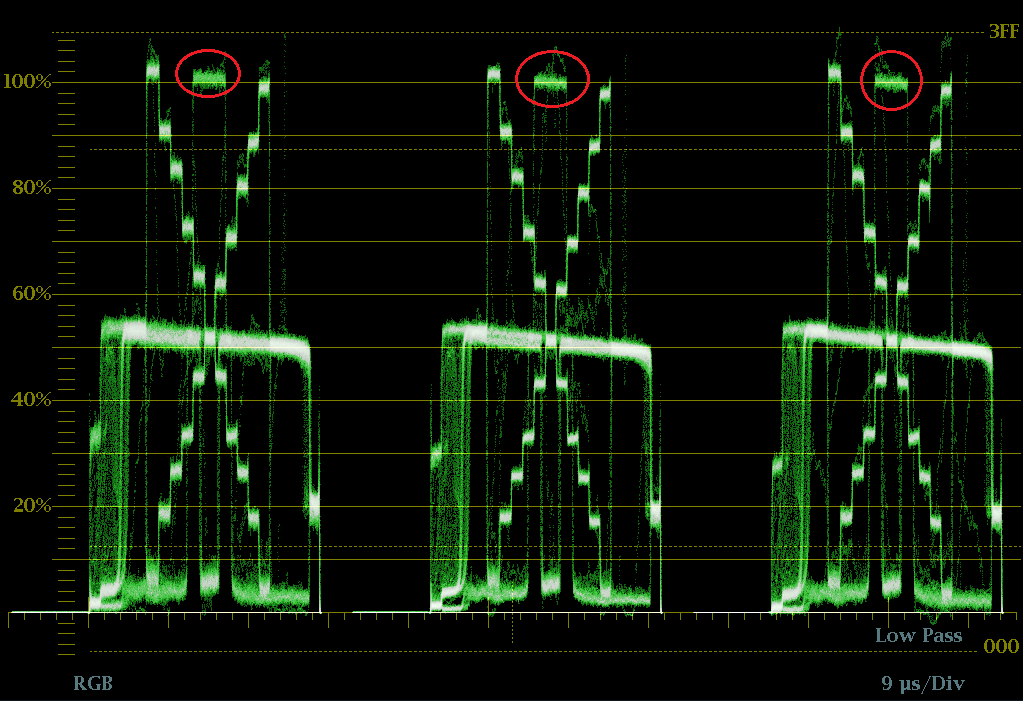
\includegraphics[width=1.0\textwidth]{bilder/arri} 
% Bilddatei aus dem Unterverzeichnis bilder holen, skalieren auf 0.8*Satzspiegel
\caption {Waveformmonitor Screenshot vom Weißabgleich des Arri D5 mit einer Grautreppe}\label{b_matrix}
\end{figure}


Die drei Abschnitte stehen von links nach rechts für die Rot-, Grün- und Blausignalanteile. Die \glqq Treppenstufen\grqq\ zeigen die Grautreppe des Bildes. Für den Weißabgleich ist entscheidend, dass alle drei Signalpegel auf 100\% eingestellt ist (mit rot gekennzeichnet), damit weiß in der Kamera auch weiß aussieht. \\
Für die Hauptmessung ist zu beachten, dass man auf diese Weise zwar jedem Scheinwerfer einen gleichen Weißwert in der Kamera geben kann. Jedoch beeinflusst diese Anpassung nicht die Farben der Scheinwerfer und lässt dadurch zum Beispiel Hauttöne natürlich aussehen. Die Farben sind weiterhin vom Spektrum der Scheinwerfer abhängig.

\section{Farbbildwandlertechnik einer Kamera}
\label{sec_wandler}
Es gibt verschiedene Arten von Farbbildwandlern, die in einer Kamera verbaut sind. Die gängigsten Methoden sind die 1- und 3-Wandlertechnik.\\
Die Sensoren von \glqq Single Sensor\grqq -Kameras arbeiten mit aufgedampften Bayer Pattern, um ein Farbbild zu erzuegen (Abbildung \ref{b_bayer}). Herr Dr. Bryce E. Bayer hat sich dabei an der V-$\Lambda$-Kurve des Auges orientiert und daher teilen die Bayer Pattern das Bild in 50\% grüne, 25\% rote und 25\% blaue Pixel auf\footnote{\cite{itwissen}}. Die fehlenden Farbanteile des Bildes werden über die Nachbarpixel interpoliert und diese gesammelten Farbinformationen dann an den Bildwandler weitergegeben.

\begin{figure}[htp]     % h=here, t=top, b=bottom, p=page
\centering
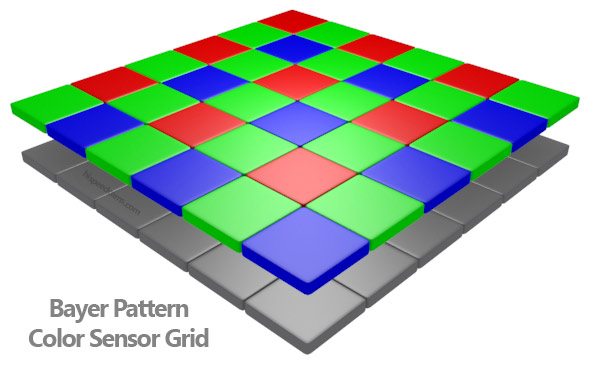
\includegraphics[width=0.6\textwidth]{bilder/bayer} 
% Bilddatei aus dem Unterverzeichnis bilder holen, skalieren auf 0.8*Satzspiegel
\caption {Bayer Pattern auf einem Kamerachip\protect\footnotemark}\label{b_bayer}
\end{figure}
\footnotetext{\url{http://www.hispeedcams.com/wp-content/uploads/2015/06/BayerPattern.jpg}}

Der Nachteil an dieser Methode ist, dass auf diese Weise die Farbauflösung der Bilder verringert wird. Daher ist eine \glqq Single Sensor\grqq -Kamera nicht geeignet, wenn das entstehende Filmmaterial auf ihre Farbigkeit überprüft werden soll.\\
Bei der 3-Wandler-Technik hingegen wird das in der Kamera ankommende Licht über Filter auf einem Strahlenteiler Prisma in die Farbwertanteile Rot, Grün und Blau aufgespalten und auf den jeweiligen Farbbildwandler durchgelassen\footnote{\cite[378]{schmidt}} (Abbildung \ref{b_wandler}). 

\begin{figure}[H]     % h=here, t=top, b=bottom, p=page
\centering
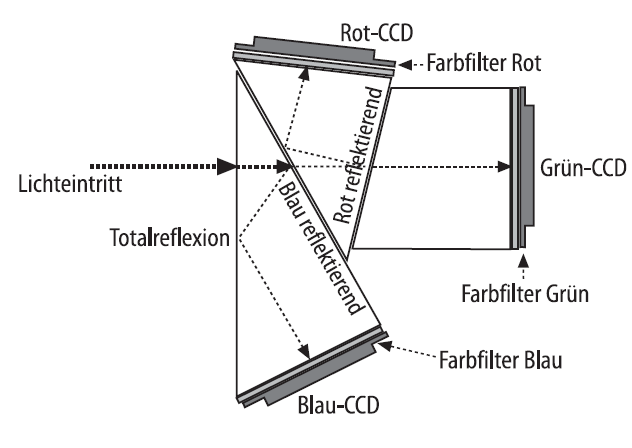
\includegraphics[width=0.6\textwidth]{bilder/wandler} 
% Bilddatei aus dem Unterverzeichnis bilder holen, skalieren auf 0.8*Satzspiegel
\caption {Schematischer Aufbau eines Farbbildwandlers\protect\footnotemark}\label{b_wandler}
\end{figure}
\footnotetext{\cite[378]{schmidt}}


Da die Filter zur Farbauftrennung nicht ideal sind und vor allendingen blaues Licht auf die nicht dafür vorgesehenen Wandler trifft, gibt es einen weiteren Farbkorrekturfilter vor jedem Wandler\footnote{\cite[379]{schmidt}}. Der Vorteil dieser Variante besteht darin, dass Bild keine Farbauflösung verliert. Die spektralen Eigenschaften eines Strahlenteilers zeigen, dass Kameras mit 3-Wandler-Technik das Licht schon \glqq vorfiltern\grqq\ (Abbildung \ref{b_twandler}). Danach wird es noch über die Farbmischkurven des Sensors weiter gewichtet (Abbildung \ref{b_matrix}). Damit wird das Licht  auf zwei Instanzen hintereinander in der Kamera unterschiedlich vom Auge bewertet.

\begin{figure}[H]     % h=here, t=top, b=bottom, p=page
\centering
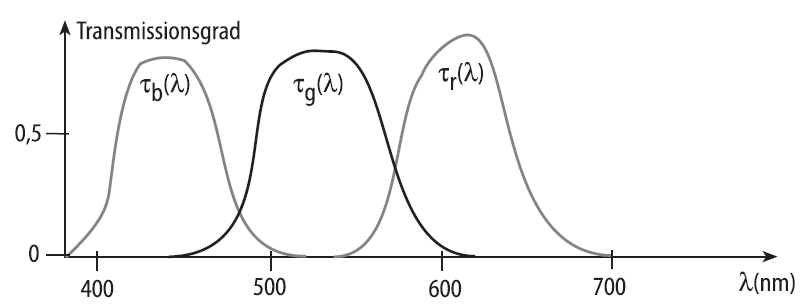
\includegraphics[width=0.6\textwidth]{bilder/twandler} 
% Bilddatei aus dem Unterverzeichnis bilder holen, skalieren auf 0.8*Satzspiegel
\caption {Transmission eines Strahlteilers\protect\footnotemark}\label{b_twandler}
\end{figure}
\footnotetext{\cite[379]{schmidt}}


\section{RGB-Signal}
\label{sec_rgbsignal}
Das unkomprimierte Kamerasignal, dass aus einer Studiokamera kommt, wird RGB-Signal genannt. Es besteht aus den drei Farbwertsignalen R,G und B. Zu diesen Signale ist anzumerken, dass es sich um elektrische Signale mit $\gamma$-Vorverzerrung handelt\footnote{\cite[82]{schmidt}}. Für diese drei Farbwertsignale sind folglich drei Übertragungskanäle nötig. 100\% Signalpegel entspricht einer Übertragungsspannung von $0,7$ V. Damit das transportierte Bild synchron bleibt, wird entweder auf einer separaten Leitung oder auch auf allen drei Leitungen mit einem Signalpegel von $-0,3$ V das Synchronsignal mitgeführt. Das RGB-Signal führt keine Qualitätsverluste mit sich, hat aber einen hohen Bandbreitenbedarf und wird daher nur auf kurzen Strecke im Studio genutzt\footnote{\cite[83]{schmidt}}.

\section{Komponenten-Signal}
\label{sec_ycrcb}
Als das Farbfernsehen erfunden wurde, gab es zwei Anforderungen an das Farbfernsehsignal, damit der Übergang vom Schwarz/Weiß-Fernsehen funktioniert: 
\begin{enumerate}
\item Das Farbfernsehsignal muss s/w kompatibel sein. Daher soll Farbfernsehsignal so gestaltet, dass man mit einem Schwarz/Weiß-Fernseher auch fernsehen ohne Farbe kann.
\item Das Farbfernsehsignal soll keine zusätzliche Bandbreite kosten, damit der Fernsehzuschauer zu Hause auch über die s/w Leitung Farbfernsehen empfangen kann
\end{enumerate}

Um diesen beiden Anforderungen gerecht werden zu können, wird das RGB-Signal dementsprechend angepasst. Um die erste Anforderung zu erfüllen, wird aus dem RGB-Signal ein Leuchtdichtesignal errechnet:

\begin{eqnarray}\label{gl_ycrcb1}
	Y = 0,299 \cdot R + 0,587 \cdot G + 0,114 \cdot B\\
	Y = 0,2126 \cdot R + 0,7152 \cdot G + 0,0722 \cdot B
\end{eqnarray}

Die erste Gleichung \ref{gl_ycrcb1} ist für das SD-Signal, die zweite Gleichung für das HD-Signal. Auch hier spricht man wieder von elektrischen Signalen die $\gamma$-vorentzerrt sind. Damit bei einer Bandbreitenreduktion nur die Farbanteile und keine Helligkeiten reduziert werden, wird neben dem Y-Signal auch ein (R-Y)- und (B-Y)- Singal übertragen. Den Farbanteilen wird also das Leuchtdichtesignal abgezogen. Dadurch wie die Helligkeit von den Farbanteilen des Signal getrennt. Es werden absichtlich R und B gewählt, da G-Y nur geringe Pegel ergibt, da Y hauptsächlich durch den Grünanteil bestimmt ist.\\ Die Pegel dieser Farbdifferenzsignale können den maximal Wert von 0,7 V bei Vollausteuerung überschreiten und müssen daher angepasst werden\footnote{\cite[84]{schmidt}} (Gleichung \ref{gl_ycrcb2}).

\begin{eqnarray}\label{gl_ycrcb2}
	C_{R}=0,713(R-Y)\\
	C_{B}=0,564(B-Y)
\end{eqnarray}

Diese Gleichungen gelten für SD-Signale. Für HD-Signale sind folgende Gleichungen anzuwenden:

\begin{eqnarray}\label{gl_ycrcb3}
	C_{R}=0,6350(R-Y)\\
	C_{B}=0,5389(B-Y)
\end{eqnarray}


Damit sind die zwei Anforderungen erfüllt. Das $YC_{R}C_{B}$-Signal ist wichtig für die Messung mit dem Vektorskop in den Hauptmessungen (Kapitel). Das Signal an sich muss noch weiter angepasst werden, damit es irgendwann ein sendefähiges Fernsehsignal wird. Diese Entwicklung ist in dieser Arbeit aber nicht mehr von Belang.



\section{Videotechnische Messgeräte}
In der Hauptmessung werden zwei videotechnische Messgeräte genutzt, um den Weißabgleich der Scheinwerfer zu überprüfen und die Farbverschiebung in der Kamera aufzuzeigen.

\subsection{Waveformmonitor}
\label{sec_wmf}
Ein Waveformmonitor ist ein Oszilloskop für die Videomessung. Oszilloskope basieren auf der Braunschen Röhre mit einem Elektronenstrahl. Dieser wiederum regt einen Bildpunkt auf der Bildschirm des Gerätes an\footnote{\cite[109]{schmidt}}.
Die Messspannung ist für die Ausrichtung des Strahls zuständig und der Elektronenstrahl kann dadurch in horizontaler (x-Achse) wie vertikaler (y-Achse) Ausrichtung beeinflusst werden. Dazu werden zwei Spannungen genutzt (Abbildung \ref{b_oszilloskop}).

\begin{figure}[H]     % h=here, t=top, b=bottom, p=page
\centering
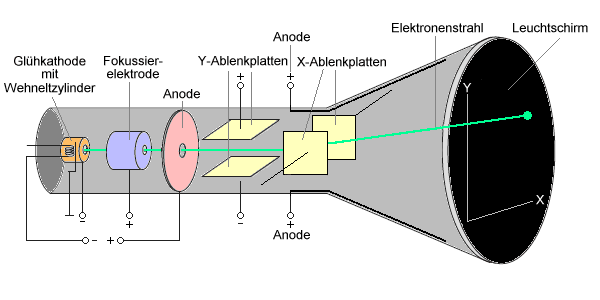
\includegraphics[width=0.9\textwidth]{bilder/oszilloskop} 
% Bilddatei aus dem Unterverzeichnis bilder holen, skalieren auf 0.8*Satzspiegel
\caption {Funktionsweise eines Oszilloskops\protect\footnotemark}\label{b_oszilloskop}
\end{figure}
\footnotetext{\url{http://www.hobby-bastelecke.de/bilder/messen/oszilloskop.gif}}

Das Messgerät misst eine Zeile des Bildes, die am Gerät ausgewählt werden kann. Bei Messungen wird normalerweise nur die y-Achse genutzt und die horizontaler Richtung wird nach festgelegten Zeit durchlaufen\footnote{\cite[110]{schmidt}}. Auf dem Bildschirm des Messgerätes wird der Pegel von 0-100 angezeigt, so wie der negative Bereich für den Synchonisationbrust bei $-0,3$V. Bei periodischen Signalen wird die Messung speziell getriggert, sodass die Pegelwerte der selben Messzeit und Phasenlänge stets übereinander liegen. Durch bestimmte Filter kann nur das Luminanzsignal, Chrominanzsignal oder beide dargestellt werden\footnote{\cite[111]{schmidt}}.\\
Bei einem Weißabgleich werden Waveformmonitore genutzt um zu überprüfen, dass unter einen bestimmen Beleuchtung alle Pegel gleich ausgesteuert sind (Abbildung \ref{b_wmf}).

\begin{figure}[H]     % h=here, t=top, b=bottom, p=page
\centering
\includegraphics[width=0.9\textwidth]{bilder/wmf} 
% Bilddatei aus dem Unterverzeichnis bilder holen, skalieren auf 0.8*Satzspiegel
\caption {Frontansicht eines Waveformmonitors der Firma Tektronix\protect\footnotemark}\label{b_wmf}
\end{figure}
\footnotetext{\url{https://www.tek.com/sites/default/files/media/image/A000_1387-L.jpg}}

Die Pegel werden von 0 mV bis 700 mV angezeigt. Die negativen Pegel (-300 mV) werden für die Synchronisation des Videosignals genutzt. Das Bild wird dabei in drei Blöcke für das Rot-, Grün- und Blausignal aufgeteilt ( von l. nach r.). Der WFM wird auch während der Hauptmessung zu Überprüfung des Videosignals genutzt.

\subsection{Vektorskop}
\label{sec_vector}
Der Farbton ist mit einem WFM-Monitor nicht gut erkennbar, da der Phasenwinkel der Farbanteilsignale des RGB-Signals im hochfrequenten Bereich schwer auslesbar sind. An dieser Stelle kommt das Vektorskop ins Spiel. Dieses Gerät wird auch mit einen Elektronenstrahl in zwei verschiedene Achsen betrieben. Im Gegensatz zum Waveformmonitor orientiert sich das Vektorskop horizontal an der U- und vertikal an der V-Komponente des FBAS-Signals. Die U- und V-Werte stammen aus dem Farbdifferzsignalen des Komponentensignals mit einer anderen Pegelreduzierung (Gleichung \ref{gl_vector1}).

\begin{eqnarray}\label{gl_vector1}
	U = 0,493(B-Y)\\
	V = 0,877(R-Y)
\end{eqnarray}

Diese Anpassung wird dadurch verursacht, dass die Farbdifferenzsignale im FBAS-Signal in modulierter Form überlagert werden und daher im Pegel reduziert werden müssen\footnote{\cite[84]{schmidt}}. Das FBAS-Signal ist eine abgewandelte Form des Komponentensignals und für diese Arbeit unrelevant.\\
Der Bildschirm eines Vektorkops ist mit sechs Toleranzflächen ausgestattet und zeigt über den ganzen Bildschirm alle Farben an. In der Mitte der Anzeige liegt der Unbuntpunkt. Der Elektrodenstrahl fährt über den Bildschirm und zeigt die Farben der Bildzeile an. Dafür wird das Vektorskop mit einem Farbbalkentestbild kalibriert. Das Farbbalkentestbild besteht aus allen sieben möglichen Kombinationen der RGB-Farbanteile (Abbildung \ref{b_te106}).

\begin{figure}[H]     % h=here, t=top, b=bottom, p=page
\centering
\includegraphics[width=0.6\textwidth]{bilder/te106} 
% Bilddatei aus dem Unterverzeichnis bilder holen, skalieren auf 0.8*Satzspiegel
\caption {\glqq TE106\grqq\ Color Bar Test Chart der Firma Image Engineering\protect\footnotemark}\label{b_te106}
\end{figure}
\footnotetext{\url{https://www.image-engineering.de/content/products/charts/te106/images/TE106.jpg}}

Abhängig davon, ob das Testbild mit vollausgesteuerten RGB-Farbanteilen (100/100) oder mit 75\% Pegelsignal erstellt wurde (75/100), wird der Synchronisationburst vom 0-Punkt aus mit einem Winkel von $135^\circ$ mit der entsprechenden Länge dargestellt. So wird dann entweder die Makierung \glqq 100\grqq\ oder \glqq 75\grqq\ getroffen (Abbildung \ref{b_vektorskop}).

\begin{figure}[H]     % h=here, t=top, b=bottom, p=page
\centering
\includegraphics[width=0.6\textwidth]{bilder/vektorskop} 
% Bilddatei aus dem Unterverzeichnis bilder holen, skalieren auf 0.8*Satzspiegel
\caption {\glqq TE106\grqq\ Darstellung der Vektorskopeinteilung mit der Q- und I-Achse\protect\footnotemark}\label{b_vektorskop}
\end{figure}
\footnotetext{\url{https://upload.wikimedia.org/wikipedia/commons/7/7b/Vectorscope_graticule.png}}

Danach werden alle Farben des Vektorkops einmal im Toleranzfeld getroffen. Eine Winkelabweichung steht im diesen Zusammenhang für einen Farbtonfehler. Mit bis zu 3\% Winkelabweichung kann der richtige Farbton noch getroffen werden. Eine Amplitudenabweichung des Signals ist ein Sättigungsfehler und wird durch die Toleranzfelder mit bis zu 5\% Abweichung anerkannt\footnote{\cite[114]{schmidt}}.

Die Vektorskopbilder aus der Vormessung zeigen zum Beispiel, wie sich die verschiedenen Beleuchtungssituation auf die Farben der Kamera auswirken (Kapitel).

\chapter{Vormessungen}

Das Ziel der Hauptmessung ist, das Licht eines 1kW Stufenlinsenscheinwerfers, der mit einem Rosco 027 \glqq Medium Red\grqq\ , Rosco 787 \glqq Marius Red\grqq\ oder Rosco 789 \glqq Blood Red\grqq\ gefiltert wird, mit dem Licht verschiedener LED-Scheinwerfer additiv zu mischen und dem Spektrum des Testscheinwerfers einen \glqq Red Tail\grqq\ anzuhängen. 
Dafür wird in den Vormessungen beobachtet wie stark dieser \glqq Red Tail\grqq\ ausgeprägt sein muss und welche Filter sich für einen \glqq Red Tail\grqq\ eignen.   
Als Beispiel wird der Clay Paky K-Eye K20 representativ für Multichip LED-Scheinwerfer für Personenlicht genommen und der Martin MAC Encore Wash CLD als Gegenstück für reinweiße LED-Engine Scheinwerfer. 
Bei den Rottönen hat man bewusst darauf geachtet, dass sich diese am Rand des Spektrums befinden. Denn Ziel des \glqq Red Tail\grqq\ ist es, dem Spektrum einen tiefroten Anteil anzuhängen, der nicht schon im gelb-orangenen Spektralbereich beginnt und ab dort den gesamtem Spektralbereich erhöht.  

\section{Aufbau und Messungen}
\label{sec_vmaum}

Für die Messung wird der Scheinwerfer direkt neben dem folierten Stufenlinsenscheinwerfer plaziert, um den Messfehler durch unterschiedliche Winkel der Scheinwerfer so gering wie möglich zu halten. Der JETI Specbos 1211, mit dem Standart Diffusor bestückt, wird als primäres Messgerät genutzt. Es wird aus 7m Entfernung direkt gemessen, damit man vergleichbare Helligkeiten erreicht (500lux). 
%Zeichnung einfügen

Den Scheinwerfern wird dann in 10\% Schritten das rotgefilterte Licht des Stufenlinsenschwerfers hinzugemischt. Die Farben des Scheinwerfers werden bei jedem Schritt erneut auf die gleiche Farbtemperatur und gleichem Abstand zum Plank'schen Kurvenzug gedreht, damit die Werte vergleichbar bleiben.


\section{Fazit aus der Vormessung}
\label{sec_vmfazit}
Die Auswirkungen des \glqq Red Tail\grqq\ wird vorallendingen in den TLCI-Werten sichtbar. Zusätzlich sind auch leichte Tendenzen bei den CQS-Werten und den TM-30-Werten bemerkbar.
Wenn man dem K-Eye K20 ein zusätzliches Rosco 027 \glqq Medium Red\grqq\ dazumischt, dann ist der \glqq Red Tail\grqq\ ab 20\% gesättigt (Abbildung \ref{b_keyevor1}). 

\begin{figure}[H]     % h=here, t=top, b=bottom, p=page
\centering
\includegraphics[width=1.0\textwidth]{bilder/keyevor1} 
% Bilddatei aus dem Unterverzeichnis bilder holen, skalieren auf 0.8*Satzspiegel
\caption {Alle 10 Spektren der Vormessung des K-Eye K20 mit einem zusätzlichen  Rosco 027 \glqq Medium Red\grqq\ (das farbige Spektrum wurde ohne zusätzlichen tiefroten Spektralanteil gemessen.)}\label{b_keyevor1}
\end{figure}

Mit 50\% zusätzlichem Rot sind die Farbwiedergabewerte so niedrig, dass der \glqq Red Tail\grqq\ eine Verschlechterung des Scheinwerfers darstellt. Dies ist eine Folge aus dem Angleichen des Scheinwerferspektrums mit einem größeren \glqq Red Tail\grqq\ .
Das zusätzliche Rot muss jedes mal mit den Farben des Scheinwerfers ausgeglichen werden, um dasselbe 6000k-Weiß zu erhalten. Abhängig von diesem neuen Mischverhältnis mit dem \glqq Red Tail\grqq\ ergibt sich entweder ein Spektrum, dass durch das Rot und die ausgleichenden Farben bereichert wurde, oder das Spektrum wurde durch die stetig größer werdenden Peaks und Einbuchtungen verzogen (Abbildung \ref{b_keyevor2}).


\begin{figure}[H]     % h=here, t=top, b=bottom, p=page
\centering
\includegraphics[width=1.0\textwidth]{bilder/keyevor2} 
% Bilddatei aus dem Unterverzeichnis bilder holen, skalieren auf 0.8*Satzspiegel
\caption {Mit 50\% \glqq Red Tail\grqq\ (farbig) wird das Spektrum schlechter. Die Roten Kreise weisen auf die entstehenden Peaks (Blau / Rot / Limette) und Täler (Amber / Cyan) hin.}\label{b_keyevor2}
\end{figure}


Mit dem Rosco 787 \glqq Marius Red\grqq\ sind analog zum 027 Filter dieselben Tendenzen erkennbar, außer dass die Sättigung des \glqq Red Tail\grqq\ erst bei 30\% erreicht ist.
Der Rosco 789 \glqq Blood Red\grqq\ Filter hingegen zeigt ein anderes Bild. Ab 30\% tritt auch hier die Sättigung des \glqq Red Tail\grqq\ ein. Eine weitere Erhöhung des zuätzliches Rotes ändert aber weder die Farbwiedergabewerte, noch machen sie eine größere Anpassung der Farben des K-Eye K20 nötig. Dieses Verhalten ist daher zu erklären, dass der Transmissionsgrad des Rosco 789 \glqq Blood Red\grqq\ Filters  $Y=1,2\%$ beträgt, also nur 1,2\% des Lichts der Stufenlinsen durchlässt. Dieser selbst gebaute \glqq Red Tail\grqq\ ist mit der Leistungsklasse eines 1kW-Leuchtmittel zu dunkel, um über den Sättigungspunkt hinauszukommen(Abbildung \ref{b_keyevor3}).  

\begin{figure}[H]     % h=here, t=top, b=bottom, p=page
\centering
\includegraphics[width=1.0\textwidth]{bilder/keyevor3} 
% Bilddatei aus dem Unterverzeichnis bilder holen, skalieren auf 0.8*Satzspiegel
\caption {Alle 10 Spektren der Vormessung des K-Eye K20 mit einem zusätzlichen  Rosco 789 \glqq Blood Red\grqq\ (das farbige Spektrum wurde ohne zusätzlichen tiefroten Spektralanteil gemessen.)}\label{b_keyevor3}
\end{figure}

Für den Mac Encore CLD Wash kann man mit dem Rosco 027 \glqq Medium Red\grqq\ eine ähnliche Tendenz wie bei dem K-Eye K20 feststellen (Abbildung \ref{b_encorevor1}. Ab 40\% kann man von einer Sättigung des \glqq Red Tail\grqq\ reden. Der Rosco 787 \glqq Marius Red\grqq\ Filter liefert erst bei 70\% eine Sättigung und zeigt so, dass schon dieser Rotton zu dunkel ist, um die Sättigungswert zu überschreiten. Weil der Rosco 789 \glqq Blood Red\grqq\ Filter noch dunkler als der 787 Filter ist und dieselben Tendenzen wie alle zusätzlichen Rottöne liefert, wird dieser Rotton nicht in den Hauptmessungen verwendet. \\
Die Tendenzen zeigen, dass der \glqq Red Tail\grqq\ vorallendingen den TLCI verbessert und den Scheinwerfern ein besseres kalteweißes Spektrum ermöglicht. In der Hauptmessung wird sich zeigen, wie sich der zusätzliche tiefrote Anteil auf andere Scheinwerfer auswirkt.

\begin{figure}[H]     % h=here, t=top, b=bottom, p=page
\centering
\includegraphics[width=1.0\textwidth]{bilder/encorevor1} 
% Bilddatei aus dem Unterverzeichnis bilder holen, skalieren auf 0.8*Satzspiegel
\caption {Alle 10 Spektren der Vormessung des MAC Encore Wash CLD mit einem zusätzlichen  Rosco 027 \glqq Medium Red\grqq\ (das farbige Spektrum wurde ohne zusätzlichen tiefroten Spektralanteil gemessen)}\label{b_encorevor1}
\end{figure}


\section{Referenzlicht}
\label{sec_reflicht}
Als Referenzlicht ist der Arri Sun 5 mit einem neuen Leuchtmittel bestimmt worden, damit man die LED-Scheinwerfer an dieses Spektrum angeleichen kann. Dieser Scheinwerfer soll durch Abstand und Zoom auch auf eine Beleuchtungsstärke von 500lux gebracht werden. Bei einem größtmöglichen Abstand von 10m ist das nur über den maximalen Zoom des Scheinwerfers möglich. Dies hat zur Folge, dass das Leuchtmittel selbst über den Reflektor des Scheinwerfers gespiegelt und \glqq rückprojeziert\grqq\ wird, dass dadurch ein dunkler Bereich in Mitten des Lichtkegels entsteht. Da man das Referenzspektrum nicht verfälschen möchte, wird bei dem Referenzlicht auf jegliche Art von Filtern verzichtet. Unter dieses Umständen kann der Arri Sun 5 nicht als Referenzlampe genutzt werden.

Daher wird in der Hauptmessung ein Arri True Blue D5 genutzt, der innerhalb von 10m, mit dem Zoom auf 500 lux angepasst, ein gutes Referenzlicht liefert, welches allerdings ca. 600K wärmer als der Arri Sun 5 ist (Abbildung \ref{b_ref}. So kommt es, dass die Vormessungen auf 6000K, die Hauptmessung jedoch auf 5395K eingemessen sind. Da nur die Tendenzen der Vormessung eine Rolle spielen und die Vormessung keine direkte Einwirkung auf die Hauptmessung hat, ist dieser Unterschied zu vernachlässigen.

\begin{figure}[H]     % h=here, t=top, b=bottom, p=page
\centering
\includegraphics[width=1.0\textwidth]{bilder/ref} 
% Bilddatei aus dem Unterverzeichnis bilder holen, skalieren auf 0.8*Satzspiegel
\caption {Spektrum des Refernenzscheinwerfers ARRI D5)}\label{b_ref}
\end{figure}


\chapter{Hauptmessung}

Für die Hauptmessungen werden vier Scheinwerfer mit Multichip-LED Engine und zwei Scheinwerfer mit reinweißer LED-Engine ausgewählt. Bei den Multichip-Scheinwerfer ist der zuvorgenannte Clay Paky K-Eye K20, mit 6 verschieden farbigen LEDs, dabei, als Alternative, der Robe Robin Dl7F Wash, mit 7 verschieden farbigen LEDs, und der weltweit verbreitete ETC Source Four LED Series 2 Lustr, ebenfalls mit 7 verschieden farbigen LEDs. Dazu kommt eine weiterer \glqq Standartscheinwerfer\grqq\ aus dem TV-Bereich: der GLP Impression X4 in der \glqq L\grqq\ - Variante. Dieser verfügt über eine rote, grüne und blaue, wie eine weiße LED in seinen LED-Arrays. Weiterhin gab es noch den Martin MAC Encore CLD Wash speziell für die Personenbeleuchtung ausgelegt mit einer reinweißen LED-Engine und den Ayrton Ghibli, ebenfalls mit einer reinweißen LED-Engine, als Beispiel für einen LED-Effektscheinwerfer. 
Mit diesen Scheinwerfern soll die Auswirkung eines \glqq Red Tail\grqq\ überprüft werden.



\section{Messaufbau und Messungen}
\label{sec_hmaufbau}
Der Messaufbau gleicht dem der in der Vormessung (Kapitel \ref{sec_vmaum}). Mit 7m Abstand werden die Scheinwerfer zum Messgerät aufgebaut und über Zoom- und Abstandsvariation auf ca. 500 lux Beleuchtungstärke eingestellt, nachdem sie auf das Arri D5-Referenzweiß abgeglichen worden sind. Es wird wiederum mit dem JETI specbos 1211 mit dem Standartdiffusor gemessen und mit dem UPRtek M350S gegenkontrolliert. Alle Scheinwerfer werden so nahe wie möglich an den 1kW Stufenlinsenscheinwerfer mit den roten Filterfolien herangestellt, um den Fehler der verschiedenen Winkel so gering wie möglich zu halten. Der zu messende Scheinwerfer ist dabei im rechten Winkel zum Messgerät angeordnet, der Stufenlinsenscheinwerfer leicht angewinkelt (Abbildung \ref{messbild1}. 

\begin{figure}[H]     % h=here, t=top, b=bottom, p=page
\centering
\includegraphics[width=1.0\textwidth]{bilder/messbild1} 
% Bilddatei aus dem Unterverzeichnis bilder holen, skalieren auf 0.8*Satzspiegel
\caption {Aufbau des \glqq Red Tail\grqq\ mit dem MAC Encore Wash CLD)}\label{b_ref}
\end{figure}

Jeder Scheinwerfer wird also auf eine Farbtemperatur von 5395K des Referenzlichts eingestellt, mit einem möglichsten geringen Abstand zur Plank'schen Kurve ($ \Delta u'v'=\pm0,0001$) und einem sehr ähnlichem Farbort, um die Messungen vergleichbar zu machen. Wenn dem Scheinwerfer ein \glqq Red Tail\grqq\ hinzugemischt wird, wird der Scheinwerfer erneut auf die Referenz angeglichen. 

%Beispiel bringen

\chapter{Messergebnisse}

Die Tendenzen zeigen, dass der Ghibli, MAC Encore, Lustr und K-Eye K20 durch den Red Tail verbessert wurden. Wie in den Vormessungen zu sehen, zeigt sich dies in allen Farbwiedergabewerten, vorallendingen aber im TLCI. Der MAC Encore kann mit einem Rosco 027 \glqq Medium Red\grqq\ im TLCI sogar um 16 Punkte verbessert werden. Diese Scheinwerfer zeigen, dass der zusätzliche \glqq Red Tail\grqq\ eine Verbesserung des Spektrums darstellt, unabhänging davon, welches zusätzliche rot genutzt wird. 
% Tabelle einfügen

Die Erklärung liegt hier wie in der Vormessung an den beiden Vorteilen des \glqq Red Tail\grqq\ : Es wird auf der einen Seite der tiefrote Bereich der Scheinwerfer aufgefüllt und zum anderen werden zum Ausgleich des zusätzlichen tiefroten Anteils wieder wertvolle Anteile in der Mitte des Spektrums dazugemischt. Spannend ist, das beim Clay Paky K-Eye K20 nur der TLCI verbessert werden konnte. Dies hängt damit zusammen, dass dem K-Eye K20 mit \glqq Red Tail\grqq\ deutlich weniger Amber zur Verfügung steht und der 645nm Rot-Peak in die Höhe schießt. Das Spektrum wird also unausgeglichener und dafür von den Farbwiedergabewerten bestraft (Abbildung \ref{b_keye1}).
\begin{figure}[H]     % h=here, t=top, b=bottom, p=page
\centering
\includegraphics[width=1.0\textwidth]{bilder/keye1} 
% Bilddatei aus dem Unterverzeichnis bilder holen, skalieren auf 0.8*Satzspiegel
\caption {Vergleich des K-Eye K20 Spektrums bei 5395 K (bunt) mit dem Spektrum eines zusätzlichen Rosco 027 \glqq Medium Red\grqq . Entstandene Unterschiede sind besonders hervorgehoben.}\label{b_keye1}
\end{figure}

Der Impression X4L konnte nicht durch ein zusätzliches rot verbessert werden. Dies liegt daran, dass das Spektrum, des X4Ls vorallendingen aus schmalbandigen Peaks besteht, die das Spektrum nicht ausfüllen (Abbildung \ref{b_impression1}). Zusätzlich kann man mit der blauen LED, das Spektrum nicht weiter ausfüllen, da der Peak der weißen LED exakt mit dem der blauen LED übereinstimmt. Auch ein Angleichen des Spektrums mit einem \glqq Red Tail\grqq\ verbessert dieses extreme Spektrum nicht, sondern vergrößert das spektrale Tief im 595nm Wellenlängebereich sogar. Ein aufgefülltes Spektrum kann also mit einem \glqq Red Tail\grqq\ bereichert werden, während man bei einem schmalbandigen Spektrum für eine Auffüllung der Randbereiche nicht belohnt wird.\\

\begin{figure}[H]     % h=here, t=top, b=bottom, p=page
\centering
\includegraphics[width=1.0\textwidth]{bilder/glp1} 
% Bilddatei aus dem Unterverzeichnis bilder holen, skalieren auf 0.8*Satzspiegel
\caption {Vergleich des Impression X4L Spektrums bei 5395 K (bunt) mit dem Spektrum eines zusätzlichen Rosco 027 \glqq Medium Red\grqq . Täler und Peaks sind besonders hervorgehoben.}\label{b_glp1}
\end{figure}


Bei dem Robe Robin DL7F haben wir im High-CRI Modus auch keine Verbesserung mit einem \glqq Red Tail\grqq\ erzielen können. Das Spektrum des Robin DL7F ist durch viele Peaks und Täler gekennzeichnet, außer im Bereich von 510nm-550nm Wellenlänge, wo das Spektrum sehr breitbandig ist (Abbildung \ref{b_dl7f1}). Durch Angleichungen an den \glqq Red Tail\grqq\ wird das Lime vermindert, das Tal im gelben Spektralbereich noch tiefer und der rot Peak wird erhört. Das Spektrum wird also noch mehr in seine Extreme verzerrt und dass wird von den Farbwiedergabewerten bestraft.

\begin{figure}[H]     % h=here, t=top, b=bottom, p=page
\centering
\includegraphics[width=1.0\textwidth]{bilder/dl7f1} 
% Bilddatei aus dem Unterverzeichnis bilder holen, skalieren auf 0.8*Satzspiegel
\caption {Vergleich des DL7F Spektrums bei 5395 K (bunt) mit dem Spektrum eines zusätzlichen Rosco 027 \glqq Medium Red\grqq . Täler und Peaks sind besonders hervorgehoben.}\label{b_dl7f1}
\end{figure}

\section{Analyse der Farbwiedergabewerte}
\label{sec_analfww}
Die Farbwiedergabewerte haben unterschiedlich stark auf den \glqq Red Tail\grqq\ reagiert. Der TLCI zeigt dabei stets den größten Ausschlag mit bis zu 16 Punkten, CQS und TM-30 erhöhen sich höchsten um 5 Punkte. Dies verwundert bei einem TM-30, der mit seinen 99 Farben folglich keine tiefrote Referenz besitzt. Jedoch ist die Verbesserung des Rotanteils stehts im roten \glqq binning\grqq\ zu erkennen(s. Kap. \ref{sec_tm30}). Ebenso ist im CQS am 1. Referenzwert der dazugekommene  
%fertig schreiben und vernünftig angucken !!


\section{Fazit aus den Hauptmessungen}
\label{sec_fazithm}
Aus den Hauptmessungen lässt sich schließen, dass der \glqq Red Tail\grqq\ tendenziell die Scheinwerfer verbessert. Am deutlichsten ist dies stets im TLCI zu erkennen, es macht sich aber ebenso im CQS, wie im TM-30 bemerkbar. Die Verbesserung ist einmal durch den zusätzlichen tiefroten Anteil im Spektrum zu erklären und dadurch, dass das Spektrum mit diesem neu angepasst wird. Bei Scheinwerfern mit schmalbandigen Spektren führt der Red Tail dazu, dass die Spektren noch extremer werden (größere Peaks, größere Täler) und so können die Farbwiedergabewerte nicht verbessert werden. Ein zu großer \glqq Red Tail\grqq\ ist nicht zu empfehlen, da es die Farbwiedergabewerte des Scheinwerfers wieder verschlechtern würde (siehe Kap. \ref{sec_vmfazit}). Daher sollte für jeden Scheinwerfer ein \glqq Red Tail\grqq\ individuell ausbalanciert werden.




\chapter{Umfrage}

\section{Anpassung der Scheinwerfer}
\label{sec_anpassunglampen}
Der nächste Schritt ist, auch über eine Kamera zu prüfen, welche Auswirkung der \glqq Red Tail\grqq\ auf das Spektrum der Scheinwerfer hat. Dazu sollen Probanden verschiedener Hauttöne mit und ohne \glqq Red Tail\grqq\ beleuchtet werden und dabei mit einer Kamera abgefilmt werden. Die so entstandenen Bilder werden dann in einer Umfrage miteinander verglichen.\\
Da eine Kamera das Spektrum eines Scheinwerfer deutlich anders bewertet als der JETI specbos 1211 (s. Kap ), gibt es drei Möglichkeiten fortzufahren:

\begin{enumerate}\setlength{\itemsep}{0ex}
\item Weißabgleich durch Scheinwerfer: Man gleicht die Kamera auf das Referenzweiß des Arris ab und dreht alle Farben der Scheinwerfer so hin, dass diese in der Kamera weiß erscheinen.
\item Weißabgleich durch Kamera: Man gleicht für jedes Bild die Kamera neu auf den Scheinwerfer an.
\item kein Weißabgleich: Man gleicht die Kamera auf das Referenzweiß des Arris ab und verwendet danach die Farbwerte der Scheinwerfer, so wie sie mit dem JETI specbos 1211 hingedreht worden sind.
\end{enumerate}

Variante 1 macht den Bezug zu den Messwerten des JETI specbos 1211 kaputt, da die auf die Kamera angepassten Scheinwerfer dann nicht mehr die selbe Farbtemperatur, den selben Abstand zu Plank'schen Kurve oder einen ähnlichen Farbort haben. Variante 2 erhält diese Werte, aber es kann nicht mehr wissenschaftlich beschrieben werden, welche Veränderung die Kamera durch den Weißabgleich am Spektrum vornimmt. So kann nicht mehr unterschieden werden, ob die Kamera nun aus dem Licht das natürlichere weiß gemacht hat, oder dies tatsächlich eine Auswirkung des \glqq Red Tail\grqq\ ist.
Variante 3 ist abzulehnen, weil die vermeintlich gleichen Lichtverhältnisse durch den JETI specbos 1211 gemessen durch die Kamera nicht als ähnliches weiß gesehen werden. Die Spektren der Scheinwerfer sind sehr unterschiedlich und werden daher auch von der Kamera so wahrgenommen.

Der Vollständigkeit halber werden alle 3 Varianten aufgezeichnet. Für die Umfrage hat man sich für die erste Variante entschieden, da ein typischer Weißabgleich im TV-Bereich genauso abläuft. Zuerst wird ein Scheinwerfer als Referenzlicht bestimmt und alle anderen Scheinwerfer werden mit der Kamera auf dieses Weiß korrigiert. 

Zu Demonstrationszwecken wird mit dem Mac Encore Wash CLD und dem K-Eye K20 mit einer Farbtafel aufgezeichnet. Über ein Vektorskop ist deutlich sichtbar, was die verschiedenen Varianten für Auswirkungen auf die Farben in der Kamera haben. Dies ist jedoch für diese Arbeit irrelevant und wird an dieser Stelle nicht weiter ausgeführt. %Anhang aufführen

\section{Auswahl der Kamera und der Probanden}
\label{sec_wahlderKamera}

Die Kamerawahl trifft auf eine Sony HDC-4300 UHD mit Weitwinkelobjektiv. Diese Kamera nutzt drei Bildwandler und keinen Bayer-Sensor. Bei einem Bayer-Sensor wird das Bild in 50\% Grünanteil 25\% Rotanteil und 25\% Blauanteil aufgeteilt. Nur diese Farbanteile werden vom Sensor gespeichert, die restlichen 50\% Grünanteile und 75\% Rot- und Blauanteile des Bilders werden aus den Nachbarpixeln interpoliert. Die Folge daraus ist eine niedrigere Farbauflösung als mit 3 Bildwandlern\footnote{\cite[380-381]{schmidt}}. Da die Bilder auf ihre Farbigkeit verglichen werden sollen, wird sich bewusst für eine Kamera mit drei Bildwandlern entschieden(Kaptitel \ref{sec_wandler}).\\

Die Probanden werden nach möglichst unterschiedlichen Hauttönen ausgewählt. Leider sind am Aufnahmetag nicht alle Probanden erschienen und daher ist die Bandbreite der Hauttöne nicht so groß wie erhofft, aber dennoch aussagekräftig genug, um die Auswirkung des Red Tail beurteilen zu können. Denn nach Khan Kapitel\ref{sec_hauttöne} ist jeder Hauttyp stark im roten Spektralbereich vertreten. Die Probanden haben einen nordischen, einen südländischen, einen normalen und einen braun-gebrannten Hauttyp (Abbildung \ref{b_umfrage1}). 

\begin{figure}[H]     % h=here, t=top, b=bottom, p=page
\centering
\includegraphics[width=1.0\textwidth]{bilder/umfrage1} 
% Bilddatei aus dem Unterverzeichnis bilder holen, skalieren auf 0.8*Satzspiegel
\caption {Bild der 4 Probanden mit dem Arri D5 Referenzlicht beleuchet}\label{b_umfrage1}
\end{figure}

 
\section{Erstellung der Bilder}
\label{sec_erstellungbilder}
Bei der Erstellung der Bilder werden die Probanden auf selber Augenhöhe nebeneinander gestellt. In der Mitte steht eine Graustufenkarte für den Weißabgleich. Nachdem die Scheinwerfer und Kamera angepasst sind, wie in Kapitel \ref{sec_anpassunglampen} beschrieben, werden die Probanden für 10 Sekunden gefilmt. Dabei wird am Anfang der Aufzeichnung ein Tablet mit den aktuellen Einstellungen der Scheinwerfer und Kamera gezeigt, damit später die Daten eindeutig zugeordnet werden können.\\
Nach den Aufzeichnungen mit den Probanden wird, nochmal die Graustufenkarte für jede Einstellung einzeln aufgezeichnet, damit man auf dem Waveformmonitor das Weiß der Scheinwerfer messen kann. Durch diesen Ablauf sind Messungenauigkeiten bei der Aufzeichnung des Waveformmonitors möglich. 

\section{Umfrage nach Rec. ITU-R  BT.500-11}
\label{sec_umfrageitu}
In der \glqq Recommendation ITU-R BT.500-11: Methodology for the subjective assessment of the 
quality of television pictures\grqq\ werden verschiedene Vorgehensweisen beschrieben, wie man die Qualität von Fernsehbildern durch Umfragen einschätzen kann. Je nach dem welches Bildmaterial man zur Verfügung hat und welche Aussage man untersuchen möchte, empfiehlt die ITU-R eine andere Methode. Da der Arri D5 zwar die Referenzleuchte für den Weißabgleich ist, aber die Scheinwerfer nicht mit diesem verglichen werden soll, wird entschieden, nach der \glqq Ratio-scaling method\grqq\ vorzugehen\footnote{\cite[10]{itu}}, eine Methode ohne Refernz. Diese findet man wiederum in dem \glqq Report ITU-R BT.1082\grqq\ von 1990 und funktioniert wie folgt:
Den Probanden werden in zufälliger Reihenfolge Bilder gezeigt. Jedes  Bild soll nach dessen Qualität beurteilt werden. Dabei wird den Probanden aber keine Skala zur Bewertung vorgegeben. Der Proband entscheidet selbst, wie er seine Skala wählt. Dazu vergibt er dem ersten Bild einen ersten Eindruck in einer Zahl ausgedrückt. Je nachdem ob ihm das darauffolgende Bild besser oder schlechter befindet, wählt er die Zahl für das zweite Bild größer, kleiner (oder gleich) der ersten Zahl. Bei der Skalierung sind dem Probanden keine Grenzen gesetzt. Wenn er ein Bild dreimal so gut wie das erste befindet, kann er dem Bild den dreifachen Wert des ersten Bildes geben. Falls Bild Nummer drei zwischen der Qualität von Bild eins und zwei liegt, darf der Proband auch mit Brüchen oder Nachkommastellen einen Wert zwischen der Zahl ein und zwei finden. Der Vorteil dieser Methode ist, das die Probanden nicht an eine vorgegebene Skala gebunden sind und mit dieser nur bestimmen, wie gut Bilder sind, sondern mit dieser freien Skala auch festlegen können, um wie viel ein Bild besser oder schlechter ist\footnote{\cite[385]{itu90}}. Um die Bewertung der Bilder verschiedener Probanden nun miteinander vergleichen zu können, müssen die vergebenen Zahlen x auf die beste Bewertung $R_{1}$ des Probanden normiert werden\footnote{\cite[387]{itu90}} (Gleichung \ref{gl_umfrage}).

\begin{equation}\label{gl_umfrage}
		X_{norm} = x \cdot \frac{100}{R_{1}}
\end{equation}
Da die Probanden nur Tendenzen mit ihren Zahlen aufzeigen, sind die einzelnen Werte $X_{norm}$ der Bilder in der Auswertung der Umfrage nicht eins zu eins vergleichbar, sondern nur mit ihr Tendenz zu den anderen Bildern zu betrachten.

\section{Aufbau und Durchführung der Umfrage} 
Die Umfrage wird in einem abgedunkelt Raum durchgeführt. Der Klasse 1 Monitor wird mit dem Jeti Specbos 1211 auf $100\frac{cd}{m^{2}}$ Leuchtdichte eingemessen und auf den Farbort der Normlichtart D65 angeglichen. Das Umgebungslicht wird mit einem Arri L7-C simuliert und  auf eine ähnliche Farbtemperatur eingestellt, damit sich die Probanden auf den kalten Bildschirm adaptieren.\\
Dem Proband wird das Verfahren aus Kapitel \ref{sec_umfrageitu}  erklärt und dann werden ihm alle Bilder zwei mal in einer zufälligen Reihenfolge gezeigt, wie von dem \glqq Report ITU-R BT.1082\grqq\ empfohlen \footnote{\cite[368]{itu90}}. Der Teilnehmer soll das einzelne Bild auf seine Natürlichkeit untersuchen und mit einer Zahl bewerten. Für jedes der 38 Bilder hat der Proband 10 Sekunden Zeit. Er kann den Ablauf jederzeit stoppen, um sich seine Zahl zu notieren, darf aber die Bilder nicht vor oder zurückschalten, da sonst die Tendenzen der Bilder kaputt gehen. Die ITU hält 15 Teilnehmer an der Umfrage für ausreichend\footnote{\cite[368]{itu90}}. Dies liegt daran, dass es nicht darum geht, ein Ergebnis bezüglich einer bestimmten Bevölkerungsgruppe zu generieren. Ziel der Umfrage ist es lediglich festzustellen, welche Auswirkung der \glqq Red Tail\grqq\ auf die optische Natürlichkeit des Bildes hat, ohne speziellen Bezug zu den Probanden. So reichen deutlich weniger Teilnehmer, als bei teilnehmerspezifischen Umfragen. Um die Statistik zu festigen haben 20 Probanden an der Umfrage teilgenommen. Eine Durchführung der Umfrage dauert ca. 15 Minuten.

% Bild einfügen
%mit Wilkens über D65 einstellung reden

\chapter{Umfrageergebnisse}
Die Tendenzen der Umfrage lassen erkennen, dass die Probanden die gezeigten Hauttöne, mit einem \glqq Red Tail\grqq\ beleuchtet, als natürlicher befinden. Dieses Verhalten zeigen die Kurven des Source Four LED Series 2 Lustr, des MAC Encore Wash CLD und des K-Eye K20 (Abbildung \ref{b_umfragetab}). 

\begin{figure}[H]     % h=here, t=top, b=bottom, p=page
\centering
\includegraphics[width=1.0\textwidth]{bilder/umfragetab} 
% Bilddatei aus dem Unterverzeichnis bilder holen, skalieren auf 0.8*Satzspiegel
\caption {Auswertung der Umfrage mit einem 95\%- Konfidenzintervall (blau und graue Kurve)}\label{b_umfragetab}
\end{figure}

Dies liegt zum einen daran, dass der zusätzliche tiefrote Anteil das Spektrum auffüllt, wo es für die Hauttöne wichtig ist (Kapitel \ref{sec_hauttöne}).
Zum anderen hilft die Anpassung an den \glqq Red Tail\grqq , dass Spektrum einwenig aufzufüllen und das Peak-Loch-Verhältnis des Scheinwerfers anzupassen. Daher werden die Bilder mit einem \glqq Red Tail\grqq\ nicht rotstichiger, sondern sie wirken durch die Anpassung eher so, wie man es in der Natur erwarten würde.

\begin{figure}[H]     % h=here, t=top, b=bottom, p=page
\centering
\includegraphics[width=1.0\textwidth]{bilder/vergleich} 
% Bilddatei aus dem Unterverzeichnis bilder holen, skalieren auf 0.8*Satzspiegel
\caption {Alle drei Bilder wurden mit dem Source Four LED Series 2 Lustr beleuchtet. Das obere Bild ist ohne \glqq Red Tail\grqq . Dem mittleren wurde ein Rosco 027 \glqq Medium Red\grqq\ dazugemischt. Das untere Bild ist mit einem zusätzlichen Rosco 787 \glqq Marius Red\grqq\ erstellt worden. Die ausgedruckten Bilder sind nicht farbecht.} \label{b_vergleich}
\end{figure}

Das extreme Spektrum des Impression X4L sticht aus der Bilderreihe hervor und wirkt auf den Bildern rotstichig (Abbildung \ref{b_umfrageglp}). Bei der Umfrage ist dieses Spektrum (mit oder ohne \glqq Red Tail\grqq) mit Abstand am besten bewertet worden. Das lässt sich darauf zurückführen, dass die Probanden ans Glühlicht gewöhnt sind. Blau- oder grünstichige Bilder von Menschen wirken krank und unnatürlich. Dagegen wirken rotstichige Bilder nicht falsch, da Menschen unter Glühlicht auch rötlicher aussehen. Außerdem wird die menschliche Haut röter, wenn man in der Sonne liegt. Man ist es also durchaus gewohnt, dass Hauttöne rötlich erscheinen und dadurch werden die Bilder des Impression X4L auch als natürlich gesehen. 

\begin{figure}[H]     % h=here, t=top, b=bottom, p=page
\centering
\includegraphics[width=1.0\textwidth]{bilder/umfrageglp} 
% Bilddatei aus dem Unterverzeichnis bilder holen, skalieren auf 0.8*Satzspiegel
\caption {Aufgezeichnetes Bild der Probanden beleuchtet mit dem Impression X4L ohne zusätzlichen tiefroten Spektralanteil.} \label{b_umfrageglp}
\end{figure}

Beim Robin DL7F ist beim dritten Bild mit dem Rosco 787 \glqq Marius Red\grqq\ ein kaputtes Bild in der Umfrage gelandet. Es ist deutlich sichtbar, dass die Kamera die Probanden zu hell darstellt und dadurch die Hauttöne sehr unnatürlich aussehen. Daher ist dieser Wert für die Umfrage ungültig. Dennoch haben die Probanden dieses Bild auch durchgehend schlecht bewertet und somit zeigt sich, dass das Verfahren des\glqq Report ITU-R BT.1082\grqq\ funktioniert. 
Wenn man dem Ghibli ein Rosco 027 \glqq Medium Red\grqq\ dazumischt, und die Werte wieder auf den Ghilbi anpasst zeigen die Hauptmessung eine Verbesserung der Werte. Dagegen wirken die Probanden bei der Umfrage matt und krank und es ist keine Verbesserung sichtbar. Dies liegt am Spektrum des Ghibli, der mit seiner reinweißen LED-Engine Probleme hat, das Spektrum auszufüllen. Dem Ghibli wäre deutlich besser geholfen, wenn man das Loch im Spektrum von 470 nm bis 510 nm Wellenlänge und den Rotbereich des Spektrums aufbessern würde. Nur einen tiefroten Anteil zu ergänzen reicht nicht aus, und das macht sich auch optisch bemerkbar.\\
Vielen Probanden ist es schwer gefallen die Bilder einzuschätzen, da sich der rechte nordische Hauttyp deutlich von den anderen Hauttypen unterscheidet. Daher ist es zu einem Konflikt in der Entscheidung gekommen, wie das Bild zu beurteilen sei, wenn der helle Hautton auf dem Bild natürlich wirkte, nicht aber die anderen Hauttypen. Anderen Probanden wiederum hat dieser Unterschied geholfen, die Bilder besser einschätzen zu können. Da die vorgeschlagene Länge einer Umfrage in dem \glqq Report ITU-R BT.1082\grqq\ eine halbe Stunde nicht überschreiten sollte hat man sich für den Vergleich aller Hauttypen gleichzeitig entschieden. Ansonsten vervierfacht sich die Anzahl der 38 Bilder und damit erhöht sich die Länge der Umfrage auf eine Stunde. 




\chapter{Fazit}
Sowohl im messtechnischen als auch im optischen Vergleich konnte mit dem \glqq Red Tail\grqq\ das Licht tendenziell verbessert werden. Dieses Verhalten zeigt sich vorallendingen beim TLCI um bis zu 16 Punkten. Ein zusätzlicher tiefroter Anteil verbessert den Scheinwerfer, wie in Kapitel \ref{sec_fazithm} dargestellt, auf der einen Seite durch den zusätzlichen Rotanteil und auf der anderen Seite durch die Anpassung an den \glqq Red Tail\grqq\ . Spektren, die sehr durch Peaks geprägt und / oder schmalbandig sind, können durch einen zusätzlichen tiefroten Spektralanteil nicht verbessert werden, da die Anpassung das Spektrum der Scheinwerfer noch extremer werden lässt (s. Daten von GLP und DL7F). Auch optisch stellt der \glqq Red Tail\grqq\ dort keine Verbesserung dar. Der Ghibli kann zwar messtechnisch verbessert werden, dies konnte aber nicht in der Umfrage festgestellt werden, weil sein Spektrum sich nicht besonders gut dafür eignet, Personen zu beleuchten. Ein TLCI von 50 zeigt dem Coloristen in der Nachbearbeitung, dass die \glqq Aufbereitung sehr zeitaufwendig\grqq\ sein wird (Kapitel \ref{sec_tlci}). Daher konnte der Ghibli optisch nicht überzeugen.\\
Der zusätzliche tiefrote Spektralanteil bei einem LED-Scheinwerfer muss also immer im Zusammenhang mit dem Spektrum des Scheinwerfers, der filmenden Kamera und den zu beleuchtenden Hauttöne gesehen werden. Die Tendenzen dieser Arbeit zeigen unter der Berücksichtigung der genannten Parameter, dass der \glqq Red Tail\grqq\ das Licht der Scheinwerfer messtechnisch verbessert und optisch Hauttöne natürlicher aussehen lässt.

  


\chapter{Ausblick}
Die Tendenzen der Messungen können durch andere Untersuchungen noch gestärkt oder gemindert werden.
Die Bilder sind beispielsweise alle mit einer Sony HDC-4300 UHD mit Weitwinkelobjektiv aufgezeichnet worden. Die Wirkung der Bilder sollte daher mit anderen Objektiven und Kameras überprüft werden. Können diese Tendenzen unabhängig vom Kameramodell und Objektiv reproduziert werden?\\
Auch bei anderen Hauttypen und Scheinwerfern gilt es den \glqq Red Tail\grqq\ zu untersuchen. Die erstellten Bilder zeigen, dass Hauttöne unterschiedlich auf das zusätzliche Rot reagieren. Kann man den tiefenroten Spektralanteil auf bestimme Hauttöne anpassen? \\
Ein ganz anderes Thema ist die Frage nach dem Weißabgleich. Die Umfrage wurde aus den Bildern gestaltet, auf denen die Scheinwerfer aufs Kameraweiß gezogen wurden. Würde die Umfrage ähnlich Ergbnisse liefern, wenn bei den Bildern die Kamera an die Scheinwerfer angepasst wurden? Ein ausgiebiger Vergleich dieser beiden Methoden kann auch eine Empfehlung für zukünftige Messverfahren im Zusammenhang mit Scheinwerfern und Kamera geben.\\
Im Zusammenhang mit der Farbtemperatur steht offen, ob der \glqq Red Tail\grqq\ für jede Farbtemperatur eine tendenzielle Verbessung der lichttechnischen Parameter hervorruft. Ist im warmweißen Farbtemperaturbereich überhaupt ein tiefroter Spektralanteil nötig? Welche Farbtemperatur ist für den \glqq Red Tail\grqq\ ideal?\\
Trotz der aufgezeigten Tendenzen bringt der \glqq Red Tail\grqq\ noch viele spannende Punkte auf, die dieses Thema fortführen könnten.   


%--------------------- VERZEICHNISSE ----------------

\listoffigures % Abbildungsverzeichnis erzeugen
\listoftables % Tabellenverzeichnis erzeugen

%--------------------- LITERATURLISTE ---------------
% Die Einträge sollen alphabetisch sortiert sein.

\begin{thebibliography}{}

% Formatierung für Internetquelle
% Grundregel: Name, Vorname (falls vorhanden), VÖ-Jahr (falls vorhanden), Titel in Anführungszeichen, URL, Datum des letzten Aufrufs
% zur Formatierung der URL unbedingt den url-Befehl benutzen!!!
\bibitem[Roskothen(2017)]{rosko}
Roskothen, Peter:
\emph{\glqq Brennweite\grqq}
\url{https://www.fotowissen.eu/brennweite/}, 12.11.2017, letzter Zugriff 10.08.2018

\bibitem[jeti(2018)]{jetii}
jeti:
\emph{\glqq specbos 1211\grqq}
\url{http://www.jeti.com/cms/index.php/instruments-55/radiometer/specbos/specbos-1211}, 2018, letzter Zugriff 15.08.2018

\bibitem[Wikipedia(2018)]{wiki}
Wikipedia:
\emph{\glqq Optisches Gitter\grqq}
\url{https://de.wikipedia.org/w/index.php?title=Optisches_Gitter&oldid=176654289}, 18.04.2018, letzter Zugriff 15.08.2018

\bibitem[ITWissen.info(2017)]{itwissen}
ITWissen.info:
\emph{\glqq BAyer-Filter\grqq}
\url{https://www.itwissen.info/Bayer-Filter-bayer-filter.html}, 09.05.2017, letzter Zugriff 10.08.2018

\bibitem[Bladowski \& Maus(2010)]{unimann}
Bladowski, Beate \& Maus, Daniel:
\emph{\glqq Farbwahrnehmung\grqq}
\url{http://irtel.uni-mannheim.de/lehre/seminararbeiten/w96/Farbe/seminar.htm#Wieviele}, 15.07.2010, letzter Zugriff 28.06.2018

\bibitem[Royer \& Houser(2015)]{royerhouser}
Royer, Micheal \& Houser Kevin:
\emph{\glqq Understanding and Applying TM-30-15\grqq}
\url{https://www.energy.gov/sites/prod/files/2015/09/f26/tm30-intro-webinar_9-15-15.pdf}, 15.09.2015, letzter Zugriff 26.06.2018

\bibitem[U.S. Department of Energy(2015)]{usdep}
U.S. Department of Energy:
\emph{\glqq Evaluating Color Rendition Using IES TM-30-15\grqq}
\url{https://www.energy.gov/sites/prod/files/2016/04/f30/tm-30_fact-sheet.pdf}, Oktober 2015, letzter Zugriff 25.06.2018

\bibitem[Commission Internationale de l'Eclairage(2007)]{CIE}
Commission Internationale de l'Eclairage:
\emph{\glqq Technical Report 177:2007 : Color Rendering of White LED Light Sources\grqq}
\url{https://de.scribd.com/document/125319182/CIE-177-2007}, 2007, letzter Zugriff 20.06.2018

\bibitem[Davis \& Ohno(2006)]{davis_ohno}
Davis, Wendy L. \& Ohno, Yoshihiro:
\emph{\glqq Development of a Color Quality Scale\grqq}
\url{http://citeseerx.ist.psu.edu/viewdoc/download?doi=10.1.1.568.8399&rep=rep1&type=pdf}, 08.02.2006, letzter Zugriff 20.06.2018

\bibitem[DocCheck Flexikon(2014)]{doccheck sko}
DocCheck Flexikon:
\emph{\glqq Skotopisches Sehen\grqq}
\url{http://flexikon.doccheck.com/de/Skotopisches_Sehen}, 24.01.2014, letzter Zugriff 18.06.2018

\bibitem[DocCheck Flexikon(2014)]{doccheck pho}
DocCheck Flexikon:
\emph{\glqq Photopisches Sehen\grqq}
\url{http://flexikon.doccheck.com/de/Photopisches_Sehen}, 10.05.2016, letzter Zugriff 18.06.2018

\bibitem[Production Partner(2018)]{production partner}
Production Partner:
\emph{\glqq Farbwiedergabe: TM-30-15, CRI und Co.\grqq}
\url{https://www.production-partner.de/basics/farbwiedergabe-tm-30-15-cri-und-co/}, 22.02.2018, letzter Zugriff 20.06.2018

\bibitem[Gigahertz-Optik(2012)]{Gigahertz}
Gigahertz-Optik:
\emph{\glqq Grundladen der Lichtmesstechnik\grqq}
\url{https://www.gigahertz-optik.de/de-de/grundlagen-lichtmesstechnik/}, 2012, letzter Zugriff 20.06.2018


% Formatierung für Aufsatz / Paper: Titel in Anführungszeichen, Zeitschriftentitel kursiv

\bibitem[Mungenast(2009)]{mungenast} 
Mungenast, Philipp:
\glqq Der Graßmannsche Farbraum\grqq ,
\url{https://www.uni-koblenz.de/~cg/ss09/Proseminar_Farbmanagement/Der\%20Grassmannsche\%20Farbraum.pdf}, 08.06.2009, letzter Zugriff 20.07.2018


\bibitem[Graßmann(1853)]{grassmann} 
Graßmann, Hermann Günther:
\glqq Zur Theorie der Farbenmischung\grqq ,2018
\emph{Annalen der Physik und Chemie} vol. 165, 1853

\bibitem[United Power Research Technology Corporation(2018)]{uprtek} 
United Power Research Technology Corporation:
\glqq Advanced MK350S Specification\grqq ,2018


\bibitem[JETI Technische Instrumente GmbH(2005)]{jeti} 
JETI Technische Instrumente GmbH:
\glqq Basics of Spectral Measurement\grqq ,05.2005

\bibitem[Vinh \& Khanh(2018)]{vinhkhanh} 
Vinh, Trinh Quang \& Kahnh, Tran Quoc:
\glqq Gutes Licht macht schön \grqq, 
\emph{Licht} vol. 3, 03.2018

\bibitem[Ohno(2005)]{ohno} 
Ohno, Yoshi:
\glqq Spectral design considerations for white LED color rendering\grqq, 
\emph{Optical Engineering} vol. 44 (11), November 2005

\bibitem[Sharma \& Wu \& Dalal(2004)]{sharwu} 
Sharma, Gaurav \& Wu, Wencheng \& Dalal, Edul N.:
\glqq The CIEDE2000 Color-Difference Formula: Implementation Notes, Supplementary Test Data, and Mathematical Observations\grqq,
\emph{COLOR research and application} vol. 30, Number 1, Februar 2005

\bibitem[Yang \& Ming \& Yu(2012)]{yangmingyu} 
Yang, Yang \& Ming, Jun \& Yu, Nenghai:
\glqq Color Image Quality Assessment Based on CIEDE2000 \grqq,
\emph{Advances in Multimedia} vol. 2012, Article ID 273723, 2012

\bibitem[Houser \& Mossman \& Smen \& Whitehead(2015)]{housmoss} 
Houser, Kevin \& Mossman, Michele \& Smet, Kevin \& Whitehead, Lorne:
\glqq Tutorial: Color Rendering and Its Applications in
Lighting\grqq, 
\emph{LEUKOS} vol. 12:7-26, 2016

\bibitem[Jiajie \& Yung \& Pecht(2014)]{jiyupe} 
Fan, Jiajie \& Yung, Winco \& Pecht, Michael:
\glqq Prognostics of Chromaticity State for Phosphor-Converted White Light Emitting Diodes Using an Unscented Kalman Filter Approach\grqq, 
\emph{Device and Materials Reliability} vol. 14, 01.03.2014

\bibitem[Royer(2016)]{royer} 
Royer, Michael P.:
\glqq IES TM-30-15 Is Approved—Now What?\grqq, 
\emph{LEUKOS} vol. 12 (1-2, 3-5), 2016


\bibitem[Dooley \& Streicher(1982)]{dooley_streicher} 
Dooley, Wesley L.  \& Streicher, Ronald D.:
\glqq M--S Stereo: A Powerful Technique for Working in Stereo\grqq, 
\emph{Journ. Audio Engineering Society} vol. 30 (10), 1982

% Formatierung für Fachbuch, Diplomarbeit o.Ä.: Titel kursiv
\bibitem[Ris(2015)]{ris}
Ris, Hans Rudolf: 
\emph{Beleuchtungstechnik für Praktiker}, 5. Aufl., VDE Verlag

\bibitem[Heinen(2012)]{heinen}
Heinen, Gerd: 
\emph{AV-Medientechnik}, 1. Aufl., Europa-Lehrmittel 2012

\bibitem[Roberts(2015)]{roberts}
Roberts, Alan: 
\emph{TELEVISION LIGHTING CONSISTENCY INDEX (TLCI-2012)}, Version 2.015e, 18.04.2015

\bibitem[Schmidt(2000)]{schmidt}
Schmidt, Ulrich: 
\emph{Professionelle Videotechnik - Grundlagen, Filmtechnik, Fernsehtechnik, Geräte- und Studiotechnik in SD, HD, DI, 3D}, 6. Aufl., Springer Vieweg 2013

\bibitem[Mueller(2014)]{mueller}
Mueller, Jens: 
\emph{Handbuch der Lichttechnik - Know-How für Film, Fernsehen, Theater, Veranstaltungen und Events}, 5. Aufl., PPVMedien 2014
 
\bibitem[Hentschel(1993)]{hentschel}
Hentschel, Hans-Jürgen: 
\emph{Licht und Beleuchtung Theorie und Praxis der Lichttechnik}, 4. Aufl., Hüthig 1994

% Formatierung für Fachbuch mit Herausgeber und mehreren Autoren
\bibitem[Spehr(2009)]{spehr}
Spehr, Georg (Hrsg.): 
\emph{Funktionale Klänge}, transcript 2009

\bibitem[Greule(2014)]{greule}
Greule, Roland (Autor):
\emph{Licht und Beleuchtung im Medienbereich}, Hanser 2015 

\bibitem[Khanh \& Bodrogi \& Vinh(2007)]{khanh}
Khanh, Tran Quoc (Autor) \& Bodrogi, Peter (Autor) \& Vinh, Trinh Quang (Autor):
\emph{Color Quality of Semiconductor and Conventional Light Sources}, Wiley-VCH 2017


% Formatierung für ein einzelnes Kapitel eines speziellen Autors aus einem Fachbuch mit mehreren Autoren
\bibitem[Sowodniok(2009)]{sowodniok}
Sowodniok, Ulrike: 
\glqq Funktionaler Stimmklang -- Ein Prozess mit Nachhalligkeit\grqq, 
in: Spehr, Georg (Hrsg.): \emph{Funktionale Klänge}, transcript 2009




% Formatierung für Aufsatz / Paper: Titel in Anführungszeichen, Zeitschriftentitel kursiv
\bibitem[Stephenson(1990)]{stephenson}
Stephenson, Uwe: 
\glqq Comparison of the Mirror Image Source Method and the Sound Particle Simulation Method\grqq, 
\emph{Applied Acoustics} vol. 29, 1990

\bibitem[ITU-R(2002)]{itu}
ITU Radiocommunication Assembly:
\emph{RECOMMENDATION ITU-R BT.500-11: Methodology for the subjective assessment of the quality of television pictures},1974-1978-1982-1986-1990-1992-1994-1995-1998-1998-2000-2002

\bibitem[ITU-R(1990)]{itu90}
ITU Radiocommunication Assembly:
\emph{Report ITU-R BT.1082: Studies Toward The Unification Of Picture Assessment Methodology},1986-1990

\end{thebibliography}

%--------------------- EIGENSTÄNDIGKEITSERKLÄRUNG ---------------
\clearpage\thispagestyle{empty}
\eigen  % im header definiert
%--------------------------------------- ENDE ------------------------------------
\end{document}
%%%%%%%%%%%%%%%%%%%%%%%%%%%%%%%%%%%%











